\documentclass[12pt,a4paper]{report}

\usepackage[utf8]{inputenc}
\usepackage[T1]{fontenc}
\usepackage{lmodern}
\usepackage{microtype}
\usepackage[a4paper,width=155mm,top=25mm,bottom=25mm]{geometry}
\usepackage{setspace}
\onehalfspacing

\usepackage{amsmath,amssymb}

\usepackage{graphicx}
\usepackage{grffile}
\graphicspath{{./}{Diagrams/}{Diagrams/CSE370/}{Diagrams/CSE471/}{Diagrams/CSE470/}}
% Preserve full image resolution (no downsampling) for sharp PDF output
\pdfimageresolution=600
\usepackage[dvipsnames,svgnames,x11names,table]{xcolor}
\usepackage{tikz}
\usetikzlibrary{arrows.meta,positioning,calc,shapes.geometric,shadows}
\usepackage{pgfplots}
\pgfplotsset{compat=1.18}

\usepackage{booktabs}
\usepackage{longtable}
\usepackage{array}
\usepackage{colortbl}
\usepackage{multirow}
\usepackage{float}
\usepackage{caption}
\captionsetup{
    labelfont={bf,small},
    textfont={small},
    skip=6pt,
    format=hang
}

\usepackage[most]{tcolorbox}

\usepackage{titlesec}

\usepackage{hyperref}
\usepackage{parskip}
\usepackage{fancyhdr}
\usepackage{enumitem}

\definecolor{PrimaryBlue}{HTML}{1A3C6E}
\definecolor{AccentBlue}{HTML}{2563EB}
\definecolor{LightBlue}{HTML}{EFF6FF}
\definecolor{MidBlue}{HTML}{DBEAFE}
\definecolor{DarkText}{HTML}{1E293B}
\definecolor{GrayText}{HTML}{64748B}
\definecolor{RowShade}{HTML}{F8FAFC}
\definecolor{RowShadeAlt}{HTML}{F1F5F9}
\definecolor{GreenAccent}{HTML}{059669}
\definecolor{AmberAccent}{HTML}{D97706}
\definecolor{RedAccent}{HTML}{DC2626}
\definecolor{VioletAccent}{HTML}{7C3AED}

\hypersetup{
    colorlinks=true,
    linkcolor=PrimaryBlue,
    filecolor=magenta,
    urlcolor=AccentBlue,
    citecolor=PrimaryBlue,
}

\titleformat{\chapter}[display]
    {\normalfont\LARGE\bfseries\color{PrimaryBlue}}
    {\chaptertitlename\ \thechapter}{20pt}{\LARGE}
    [\vspace{4pt}{\color{AccentBlue}\titlerule[1.2pt]}]

\titleformat{\section}
    {\large\bfseries\color{PrimaryBlue!85!black}}
    {\thesection}{0.8em}{}

\titleformat{\subsection}
    {\normalsize\bfseries\color{PrimaryBlue!70!black}}
    {\thesubsection}{0.6em}{}

\titlespacing*{\chapter}{0pt}{-20pt}{20pt}
\titlespacing*{\section}{0pt}{16pt plus 3pt minus 2pt}{8pt plus 2pt minus 1pt}
\titlespacing*{\subsection}{0pt}{12pt plus 2pt minus 1pt}{6pt plus 1pt minus 1pt}

\newcommand{\tableheadcolor}{\rowcolor{PrimaryBlue!12}}
\newcommand{\tableheadfont}{\bfseries\small\color{PrimaryBlue}}

\newenvironment{moderntable}[1][H]{%
    \begin{table}[#1]\centering\small%
    \renewcommand{\arraystretch}{1.35}%
}{%
    \end{table}%
}

\newtcolorbox{layerbox}[1]{
    colback=LightBlue,
    colframe=AccentBlue,
    coltitle=white,
    fonttitle=\bfseries\small,
    title=#1,
    boxrule=0.8pt,
    arc=3pt,
    left=6pt,right=6pt,top=4pt,bottom=4pt,
    drop shadow={opacity=0.15},
}

\newtcolorbox{highlightbox}[1][]{
    colback=LightBlue,
    colframe=AccentBlue!60,
    boxrule=0.6pt,
    arc=2pt,
    left=8pt,right=8pt,top=6pt,bottom=6pt,
    #1
}

\pagestyle{fancy}
\fancyhf{}
\renewcommand{\headrulewidth}{0.4pt}
\fancyhead[L]{\small\color{GrayText}Crypto World Bank}
\fancyhead[R]{\small\color{GrayText}BRAC University}
\fancyfoot[C]{\small\color{GrayText}\thepage}

\begin{document}

%% ============================================================
%% TITLE PAGE
%% ============================================================
\thispagestyle{empty}

\begin{center}

\vspace*{0.5cm}


\includegraphics[width=3.8cm]{bracu_logo_12-0-2022.png}

\vspace{1.2cm}

{\LARGE\bfseries\color{PrimaryBlue} Decentralized Crypto World Bank}\\[0.5em]
{\large\color{PrimaryBlue!80} A Blockchain-Based Lending Platform\\[0.2em]with AI-Enhanced Security}

\vspace{2cm}

{\large by}

\vspace{0.8cm}

{\Large\bfseries\color{PrimaryBlue} Md.\ Bokhtiar Rahman Juboraz}\\[0.2em]
{\color{GrayText}20301138}\\[1em]
{\Large\bfseries\color{PrimaryBlue} Md.\ Mahir Ahnaf Ahmed}\\[0.2em]
{\color{GrayText}20301083}

\vspace{2cm}

A pre-thesis 1 report submitted to the Department of Computer Science and Engineering\\
in partial fulfillment of the requirements for the degree of\\
\textbf{B.Sc.\ in Computer Science}

\vfill

{\color{PrimaryBlue}\rule{0.4\textwidth}{0.6pt}}\\[0.8em]
Department of Computer Science and Engineering\\
\textbf{Brac University}\\
February 2026

\vspace{1cm}

{\small\color{GrayText}\copyright\ 2026.\ Brac University --- All rights reserved.}

\end{center}

%% ============================================================
%% DECLARATION
%% ============================================================
\newpage
\thispagestyle{empty}

\chapter*{Declaration}
\addcontentsline{toc}{chapter}{Declaration}

It is hereby declared that

\begin{enumerate}
\item The report submitted is our own original work while completing degree at Brac University.

\item The report does not contain material previously published or written by a third party, except where this is appropriately cited through full and accurate referencing.

\item The report does not contain material which has been accepted, or submitted, for any other degree or diploma at a university or other institution.

\item We have acknowledged all main sources of help.
\end{enumerate}

\vspace{2cm}

\textbf{Student's Full Name \& Signature:}

\vspace{2cm}

\begin{tabular}{p{6cm}p{1cm}p{6cm}}
\hrulefill & & \hrulefill \\
\centering Md. Bokhtiar Rahman Juboraz & & \centering Md. Mahir Ahnaf Ahmed \tabularnewline
\centering 20301138 & & \centering 20301083 \tabularnewline
\end{tabular}

%% ============================================================
%% APPROVAL
%% ============================================================
\newpage
\thispagestyle{empty}

\chapter*{Approval}
\addcontentsline{toc}{chapter}{Approval}

The pre-thesis 1 report of final year project titled ``Decentralized Crypto World Bank: A Blockchain-Based Lending Platform with AI-Enhanced Security'' submitted by

\begin{enumerate}
\item Md. Bokhtiar Rahman Juboraz (20301138)
\item Md. Mahir Ahnaf Ahmed (20301083)
\end{enumerate}

Of Spring, 2026 has been accepted as satisfactory in partial fulfillment of the requirement for the degree of B.Sc. in Computer Science on February 20, 2026.

\vspace{1cm}

\textbf{Examining Committee:}

\vspace{1.5cm}

\begin{flushleft}
Supervisor:\\
(Member)
\end{flushleft}

\begin{flushright}
\vspace{-0.5cm}
\hrulefill\\
Mr. Annajiat Alim Rasel\\
Senior Lecturer\\
Department of Computer Science and Engineering\\
Brac University
\end{flushright}

\vspace{1.5cm}

\begin{flushleft}
Pre-Thesis Coordinator:\\
(Member)
\end{flushleft}

\begin{flushright}
\vspace{-0.5cm}
\hrulefill\\
\mbox{[Pre-Thesis Coordinator Name]}\\
\mbox{[Designation]}\\
Department of Computer Science and Engineering\\
Brac University
\end{flushright}

\vspace{1.5cm}

\begin{flushleft}
Head of Department:\\
(Chair)
\end{flushleft}

\begin{flushright}
\vspace{-0.5cm}
\hrulefill\\
Dr. Sadia Hamid Kazi\\
Chairperson and Associate Professor\\
Department of Computer Science and Engineering\\
Brac University
\end{flushright}

%% ============================================================
%% ETHICS STATEMENT
%% ============================================================
\newpage
\thispagestyle{empty}

\chapter*{Ethics Statement}
\addcontentsline{toc}{chapter}{Ethics Statement}

This project operates exclusively on public blockchain test networks using test tokens with no real monetary value. No real financial transactions, personal banking data, or user financial records are involved at any stage of development or evaluation. All transaction data used for Artificial Intelligence and Machine Learning (AI/ML) model training and evaluation is either synthetically generated or sourced from publicly available anonymized datasets. The platform prototype does not process Know Your Customer (KYC) or Anti-Money Laundering (AML) data in its current scope, and all wallet addresses used during testing are disposable testnet addresses. We acknowledge the ethical considerations inherent in AI-assisted financial decision-making and have incorporated explainability mechanisms (SHapley Additive exPlanations, or SHAP) to ensure that automated risk assessments remain transparent and auditable by human reviewers.

%% ============================================================
%% ABSTRACT
%% ============================================================
\newpage
\thispagestyle{empty}

\chapter*{Abstract}
\addcontentsline{toc}{chapter}{Abstract}

Global development finance relies on multilayered institutional structures to distribute capital across borders and communities, yet these systems often struggle with fragmented transparency, procedural friction, and uneven access to credit. Although decentralized finance has demonstrated that programmable infrastructures can automate lending and enhance auditability, existing models largely employ flat architectures that do not reflect institutional hierarchies or structured governance. As a result, there remains limited exploration of how tiered financial systems might be represented within decentralized environments while preserving oversight and adaptability. Here we present \textit{Crypto World Bank}, a prototype framework that models a multi-tier institutional lending architecture on a programmable blockchain infrastructure. We show that hierarchical capital flows, role-based governance, and data-informed risk analytics can be coordinated within a unified smart contract environment, enabling transparent state visibility alongside adaptive decision support. This hybrid design illustrates how institutional finance and decentralized systems may converge, suggesting a pathway toward more accountable, flexible, and inclusive digital credit ecosystems.

\vspace{0.5em}
\noindent\textbf{Keywords:} Blockchain, Decentralized Finance, Institutional Architecture, Financial Inclusion, Smart Contracts, AI-Augmented Governance

%% ============================================================
%% DEDICATION
%% ============================================================
\newpage
\thispagestyle{empty}

\chapter*{Dedication}
\addcontentsline{toc}{chapter}{Dedication}

\vspace{3cm}
\begin{center}
\textit{Dedicated to our families for their unwavering support throughout our academic journey.}
\end{center}

%% ============================================================
%% ACKNOWLEDGMENT
%% ============================================================
\newpage
\thispagestyle{empty}

\chapter*{Acknowledgment}
\addcontentsline{toc}{chapter}{Acknowledgment}

We would like to express our sincere gratitude to our supervisor, Mr.\ Annajiat Alim Rasel, Senior Lecturer at the Department of Computer Science and Engineering, Brac University, for his guidance and support throughout this project. We also thank the Department of Computer Science and Engineering at Brac University for providing us with the resources and academic environment to pursue this work.

%% ============================================================
%% TABLE OF CONTENTS, LIST OF TABLES, LIST OF FIGURES
%% ============================================================
\newpage
\setcounter{page}{1}
\pagenumbering{roman}
\tableofcontents
\newpage
\listoftables
\newpage
\listoffigures
\newpage
\pagenumbering{arabic}
\setcounter{page}{1}


%% %%%%%%%%%%%%%%%%%%%%%%%%%%%%%%%%%%%%%%%%%%%%%%%%%%%%%%%%%%%%
%% CHAPTER 1: INTRODUCTION
%% %%%%%%%%%%%%%%%%%%%%%%%%%%%%%%%%%%%%%%%%%%%%%%%%%%%%%%%%%%%%
\chapter{Introduction}

The convergence of blockchain technology, decentralized finance, and artificial intelligence presents new opportunities to address longstanding inefficiencies in global development finance. This project, the Crypto World Bank, explores how a decentralized lending platform with a multi-tier institutional structure can improve transparency, reduce settlement friction, and expand access to credit in underserved markets. The complete source code, smart contracts, and supplementary documentation for this project are available in our \href{https://github.com/Yuvraajrahman/Cryto-World-Bank}{GitHub repository}.

We position blockchain in this context as a coordination technology that provides shared state visibility, tamper-evident audit trails, and programmable process enforcement across multiple institutions. The platform further addresses governance design, security controls, and regulatory considerations through a phased deployment pathway involving academic validation and regulatory sandbox pilots. By integrating a four-tier institutional hierarchy with transparent ledger infrastructure and data-driven risk analytics, the Crypto World Bank explores a hybrid architecture for institutional decentralized finance that targets improved operational efficiency and expanded access to credit in emerging markets.

\section{Background}

International development finance is delivered through layered institutional structures in which multilateral development institutions (e.g., World Bank, International Monetary Fund), national financial intermediaries, and local lenders jointly channel capital to end borrowers. While this model enables risk distribution and local market access, it is associated with operational challenges: limited cross-tier transparency, lengthy cross-border settlement processes, high reconciliation and compliance overhead, and constrained scalability of risk assessment workflows.

Simultaneously, approximately 1.4 billion adults remain unbanked globally according to the World Bank Global Findex~[14], highlighting the need for more efficient and accessible credit delivery mechanisms. The DeFi ecosystem has demonstrated that smart contract platforms can automate lending with full transparency; however, existing DeFi protocols employ flat, pool-based architectures that do not model institutional hierarchy or integrate AI-driven risk analytics.

\section{Rationale of the Study}

This study is motivated by the convergence of three factors: (1)~the persistent inefficiencies in traditional development finance that limit transparency and settlement speed; (2)~the gap between DeFi's technical capabilities and its failure to address multi-tier institutional lending use cases; and (3)~the opportunity to combine blockchain's auditability with AI/ML security analytics to improve both operational efficiency and decision quality. By designing a prototype that bridges these domains, we aim to demonstrate a viable path toward transparent, programmable, and AI-augmented lending for underserved populations.

\section{Problem Statement}

The global development finance ecosystem is characterized by a hierarchical topology in which supranational entities (e.g., the World Bank, International Monetary Fund) allocate capital to sovereign national institutions, which in turn disburse funds to regional and local banking entities, ultimately reaching end-user borrowers. This multi-layered intermediation introduces several systemic inefficiencies:

\begin{enumerate}[noitemsep]
\item \textbf{Opacity of ledger state.} Internal bookkeeping across tiers is not publicly auditable. Stakeholders at lower tiers have limited visibility into reserve adequacy, approval criteria, and fund utilization at higher tiers.

\item \textbf{Settlement latency.} Cross-border capital transfers between tiers involve multiple intermediaries, compliance checkpoints, and reconciliation processes, resulting in settlement periods ranging from days to weeks.

\item \textbf{Manual risk assessment.} Creditworthiness evaluation and fraud detection are predominantly human-driven, introducing inconsistency, bias, and scalability constraints.

\item \textbf{Trust deficit.} The effort required to establish inter-institutional trust through legal agreements, audit engagements, and compliance certifications constitutes a significant overhead that disproportionately affects smaller institutions and borrowers in developing economies.
\end{enumerate}

Simultaneously, the DeFi ecosystem has demonstrated that smart contract platforms can automate lending, collateral management, and interest computation with full transparency. However, existing DeFi protocols (e.g., Aave, Compound, MakerDAO) exhibit fundamental limitations in this context:

\begin{itemize}[noitemsep]
\item They employ \textbf{peer-to-pool} or \textbf{over-collateralized} lending models that do not accommodate institutional hierarchies.
\item They lack integration with \textbf{AI-driven risk analytics} and \textbf{explainable decision support} systems.
\item They do not model \textbf{role-based, tiered governance} analogous to development finance institutions.
\end{itemize}

\section{Objectives}

The objectives of this project are:

\begin{enumerate}[noitemsep]
\item To design and implement a four-tier lending architecture (World Bank $\to$ National Bank $\to$ Local Bank $\to$ Borrower) on an EVM-compatible blockchain that preserves institutional hierarchy while enabling shared ledger visibility.
\item To integrate off-chain AI/ML security analytics---including fraud detection (Random Forest), anomaly identification (Isolation Forest), and explainable risk assessment (SHAP)---to augment human credit governance.
\item To demonstrate transparent, programmable lending workflows with configurable borrowing limits, installment schedules, and role-based access control enforced by smart contracts.
\item To validate the prototype on public testnets (Polygon, Ethereum Sepolia) with functional verification of hierarchical controls, transparency properties, and operational workflows.
\item To document governance design, security controls, regulatory considerations, and a phased deployment pathway for academic validation and potential regulatory sandbox pilots.
\end{enumerate}

\section{Blockchain Justification}

The problem described above is fundamentally a \textbf{multi-party coordination and trust challenge} involving disparate institutions with potentially misaligned incentives. We assert that blockchain technology addresses this class of problems more effectively than any conventional alternative for the following reasons:

\begin{enumerate}[noitemsep]
\item \textbf{Trust minimization through consensus.} Distributed consensus mechanisms ensure that no single party can unilaterally alter the ledger state, eliminating the need for a trusted central operator.

\item \textbf{Programmable enforcement.} Smart contracts codify lending rules---borrowing limits, installment schedules, approval workflows---as deterministic, self-executing programs, reducing reliance on manual processes and bilateral agreements.

\item \textbf{Cryptographic auditability.} All state transitions are recorded in an immutable, publicly verifiable transaction log, enabling real-time auditing by regulators, partners, and borrowers without requiring costly third-party engagements.

\item \textbf{Composable incentive structures.} On-chain reputation systems, governance tokens, and programmable fee distributions can align incentives across all network participants.
\end{enumerate}

A conventional cloud-hosted database infrastructure would necessitate a trusted central operator to maintain ledger integrity, enforce access control, and provide audit guarantees---reintroducing the very trust dependencies that this project seeks to mitigate. Blockchain eliminates this single point of trust failure.

\section{Proposed Solution}

The Crypto World Bank implements a \textbf{four-tier, on-chain lending architecture}:

\begin{itemize}[noitemsep]
\item \textbf{Tier 1 --- World Bank:} Maintains the global crypto reserve. Allocates capital to registered National Banks through smart contract-mediated lending operations.
\item \textbf{Tier 2 --- National Banks:} Borrow from the World Bank reserve. Lend to registered Local Banks within their jurisdiction. Aggregate risk exposure at the national level.
\item \textbf{Tier 3 --- Local Banks:} Borrow from National Banks. Process loan requests from individual borrowers. Employ designated approvers for loan lifecycle management.
\item \textbf{Tier 4 --- Borrowers:} Submit loan requests to Local Banks. Repay through configurable installment schedules. Accumulate on-chain repayment history that informs future borrowing limits.
\end{itemize}

The platform further integrates:

\begin{itemize}[noitemsep]
\item \textbf{Risk-aware borrowing limits} computed from rolling 6-month and 1-year transaction windows.
\item \textbf{Automatic installment generation} for loan amounts exceeding a configurable threshold (e.g., 100 ETH equivalent).
\item \textbf{Off-chain AI/ML security analytics} for fraud detection (Random Forest), anomaly identification (Isolation Forest), and explainable risk assessment (SHAP).
\end{itemize}

\subsection{Cross-Tier Lending System}

In traditional banking, capital does not flow strictly top-down. Banks at the same level routinely lend to each other through the interbank lending market (e.g., the federal funds market), and lower-tier banks with surplus reserves deposit excess capital upward with their parent institutions or central banks. The Crypto World Bank extends its hierarchical architecture to support these \textbf{multi-directional lending flows}, creating a more realistic and resilient financial ecosystem.

\subsubsection{Same-Tier Lending}

Banks at the same hierarchical level can lend to one another to manage short-term liquidity:

\begin{itemize}[noitemsep]
\item \textbf{National Bank $\leftrightarrow$ National Bank:} A national bank with excess reserves can lend to another experiencing a liquidity shortfall, analogous to the traditional interbank lending market. The lending rate floats based on supply and demand across national banks in the system, similar to the Secured Overnight Financing Rate (SOFR).
\item \textbf{Local Bank $\leftrightarrow$ Local Bank:} Local banks within the same or different national jurisdictions can share liquidity through a peer lending pool. This prevents localized liquidity crunches when one bank has excess deposits while another faces elevated loan demand.
\end{itemize}

Same-tier lending is implemented through an on-chain \textbf{InterBankLendingPool} contract at each tier level, where banks with surplus offer short-term liquidity and banks with deficit can borrow at utilization-based floating rates.

\subsubsection{Upward Lending}

Lower-tier banks with surplus capital can lend upward through the hierarchy:

\begin{itemize}[noitemsep]
\item \textbf{Local Banks $\to$ National Banks:} When local banks accumulate reserves beyond their minimum reserve ratio, they can deposit surplus capital into their parent national bank's liquidity pool, earning a deposit yield. This mirrors how commercial banks deposit excess reserves with central banks through standing deposit facilities.
\item \textbf{National Banks $\to$ World Bank:} National banks can contribute surplus to the global reserve, strengthening the system's overall capital base. This provides a return channel for well-capitalized national banks and increases the reserve available for downward distribution to banks with higher demand.
\end{itemize}

Upward lending rates are lower than downward lending rates (reflecting the lower risk of lending to a higher-tier institution), creating a natural interest rate term structure across the hierarchy.

\subsubsection{Tiered Borrower Access}

Different borrower classes access different tiers based on loan size and organizational type:

\begin{moderntable}
\caption{Borrower tier access rules.}
\begin{tabular}{@{} >{\raggedright}p{3cm} >{\raggedright}p{3.5cm} >{\raggedright}p{2.5cm} >{\raggedright\arraybackslash}p{3cm} @{}}
\toprule
\tableheadfont Borrower Type & \tableheadfont Accessible Tiers & \tableheadfont Loan Range & \tableheadfont Use Case \\
\midrule
\rowcolor{RowShade}
Individual / End User & Local Bank only & 0.01--10 ETH & Personal, micro-enterprise \\
Small Business / SME & Local Bank, National Bank & 1--100 ETH & Working capital, equipment \\
\rowcolor{RowShade}
Large Corporate & National Bank, World Bank & 50--10,000 ETH & Infrastructure, large projects \\
Institutional / Sovereign & World Bank only & 1,000+ ETH & Development programs \\
\bottomrule
\end{tabular}
\end{moderntable}

End users and retail borrowers access the system exclusively through Local Banks, preserving the hierarchical intermediation model. Large corporate accounts and institutional borrowers can access higher tiers directly, subject to enhanced verification (on-chain credit history combined with off-chain documentation) and a borrower class designation in the smart contract that determines tier access permissions.

This multi-directional lending model---combining downward capital distribution, same-tier interbank lending, upward surplus repatriation, and tiered borrower access---creates a more complete representation of real-world banking flows within the decentralized architecture.

\section{Methodology in Brief}

We adopted a lightweight Agile/Scrum methodology with three sprints over an 8-week development window. Sprint~1 establishes smart contracts, frontend scaffolding, wallet integration, and database schema. Sprint~2 delivers lending features (loan requests, approvals, installments, borrowing limits), chat system, income verification, and bank registration. Sprint~3 integrates AI/ML fraud detection, risk dashboard, security audit, and documentation. Development uses Solidity~0.8.20 for smart contracts, React~18 with TypeScript for the frontend, FastAPI for the backend, and scikit-learn for ML models. We deploy on Polygon and Ethereum testnets at zero real-cryptocurrency cost.

\section{Scopes and Challenges}

\textbf{Scope.} Our prototype operates exclusively on public testnets (no real cryptocurrency). In-scope features include: four-tier lending, loan request and approval workflow, installment payments, borrowing limit computation, borrower--bank chat, income verification, fraud detection (Random Forest + SHAP), and anomaly detection (Isolation Forest). The dual-currency facility is designed as an auxiliary add-on to existing banking infrastructure. Out of scope for the prototype: mainnet deployment, fiat on-ramp/off-ramp integration, KYC/AML compliance automation, and production-scale stress testing.

\textbf{Challenges.} Key challenges include: (1)~\textit{Data scarcity}---labeled fraud data for DeFi lending is limited; synthetic or transfer learning may be required. (2)~\textit{Regulatory uncertainty}---crypto lending faces jurisdictional restrictions; our prototype mitigates this by operating on testnets only. (3)~\textit{Gas cost sensitivity}---complex on-chain logic increases transaction cost; the design partitions AI/ML and heavy computation off-chain. (4)~\textit{Model interpretability}---regulatory requirements for explainable lending decisions are addressed via SHAP-based feature attribution.

\section{Market Analysis and Partnership Ecosystem}

\subsection{Market Sizing}

\begin{moderntable}
\caption{Market segments.}
\begin{tabular}{@{} >{\raggedright}p{4cm} >{\raggedright}p{5cm} >{\raggedright\arraybackslash}p{3cm} @{}}
\toprule
\tableheadfont Segment & \tableheadfont Description & \tableheadfont Estimated Scale \\
\midrule
\rowcolor{RowShade}
Total Addressable Market (TAM) & Global decentralized lending market; DeFi lending TVL has historically exceeded \$50B & \$50B+ \\
Serviceable Addressable Market (SAM) & Institutional and semi-institutional lending requiring hierarchical structures & \$5--10B \\
\rowcolor{RowShade}
Serviceable Obtainable Market (SOM) & Pilot deployments in regulatory sandboxes, academic prototypes, NGO-backed microfinance & \$50--200M \\
\bottomrule
\end{tabular}
\end{moderntable}

\vspace{4pt}
\noindent\textit{\small\textbf{Sources:} (a)~TAM: DefiLlama [19] tracks DeFi TVL; lending protocols have historically exceeded \$50B in total value locked; (b)~SAM and SOM: Project-derived estimates based on industry segmentation of institutional/semi-institutional lending and pilot/regulatory sandbox addressable market [20].}

The market for \textbf{transparent, hierarchy-preserving decentralized lending} is presently unaddressed by existing DeFi protocols, which universally adopt flat, pool-based architectures. This represents a significant whitespace opportunity.

\subsection{Target Customer Segment}

The Crypto World Bank targets the \textbf{retail customer segment} --- individual borrowers and small businesses seeking transparent, accessible crypto-based lending services.

\begin{moderntable}
\caption{Target customer segment profile.}
\begin{tabular}{@{} >{\raggedright}p{3.8cm} >{\raggedright\arraybackslash}p{8.2cm} @{}}
\toprule
\tableheadfont Characteristic & \tableheadfont Description \\
\midrule
\rowcolor{RowShade}
Primary Users & Individual retail borrowers seeking personal or small business loans \\
Geographic Focus & Developing economies with limited traditional banking access (e.g., Bangladesh, Southeast Asia, Sub-Saharan Africa) \\
\rowcolor{RowShade}
Loan Size Range & Micro to mid-range: 0.1 ETH -- 500 ETH equivalent (\textasciitilde\$200 -- \$1,000,000 at current rates) \\
User Profile & Digitally literate individuals with cryptocurrency wallet access; small business owners; gig-economy freelancers \\
\rowcolor{RowShade}
Key Pain Points & High interest rates from informal lenders; lack of credit history in traditional systems; exclusion from banking due to documentation barriers \\
\bottomrule
\end{tabular}
\end{moderntable}

\textbf{Why Retail:} The retail segment represents the largest underserved population in developing economies. According to the World Bank's Global Findex Database, approximately 1.4 billion adults remain unbanked, with the majority concentrated in developing countries. By targeting retail customers, the platform maximizes financial inclusion impact while generating the transaction volume necessary to sustain the lending ecosystem. The hierarchical banking model (World Bank $\to$ National $\to$ Local $\to$ Borrower) mirrors how traditional microfinance institutions reach retail customers in underserved regions, but with blockchain-enforced transparency and AI-enhanced risk assessment.

\subsection{Partner Ecosystem}

\begin{moderntable}
\caption{Partner categories and roles.}
\begin{tabular}{@{} >{\raggedright}p{3.2cm} >{\raggedright}p{4.2cm} >{\raggedright\arraybackslash}p{4.6cm} @{}}
\toprule
\tableheadfont Partner Category & \tableheadfont Functional Role & \tableheadfont Blockchain-Mediated Incentive \\
\midrule
\rowcolor{RowShade}
Financial Regulators & Regulatory sandbox approval; compliance oversight & Reduced enforcement cost through on-chain transparency and audit trails \\
Banking Institutions & Network membership as National/Local Banks & Access to diversified global reserve; reduced inter-bank settlement friction \\
\rowcolor{RowShade}
Payment Gateway Providers & Fiat-to-crypto on-ramp and off-ramp services & Volume-based transaction fees; expanded market reach \\
Academic \& Research Institutions & Validation of AI/ML models; publication of research findings & Access to anonymized datasets; collaborative research opportunities \\
\rowcolor{RowShade}
Non-Governmental Organizations & Pilot deployment; field testing with underserved borrower populations & Transparent, low-friction credit access for beneficiaries \\
\bottomrule
\end{tabular}
\end{moderntable}

\subsection{Incentive Alignment Through the Blockchain Platform}

Partner incentives are allocated and enforced through the blockchain platform itself:

\begin{itemize}[noitemsep]
\item \textbf{Immutable repayment records} serve as on-chain reputation signals, enabling data-driven credit decisions without third-party credit bureaus.
\item \textbf{Transparent reserve verification} allows partners to independently confirm that allocated capital is deployed as committed.
\item \textbf{Programmable fee structures} (future extension) distribute transaction fees proportionally to network participants based on their contribution to lending volume and governance.
\end{itemize}


%% %%%%%%%%%%%%%%%%%%%%%%%%%%%%%%%%%%%%%%%%%%%%%%%%%%%%%%%%%%%%
%% CHAPTER 2: LITERATURE REVIEW
%% %%%%%%%%%%%%%%%%%%%%%%%%%%%%%%%%%%%%%%%%%%%%%%%%%%%%%%%%%%%%
\chapter{Literature Review}

\section{Preliminaries}

This section establishes key terminology and concepts used throughout the literature review and the project design.

\hangindent=0.5in \textbf{Decentralized Finance (DeFi).} DeFi refers to financial services built on blockchain platforms that operate without traditional intermediaries. Lending protocols enable users to borrow and lend assets through smart contracts, with interest rates typically determined algorithmically or by market utilization.

\hangindent=0.5in \textbf{Smart contracts.} Self-executing programs deployed on a blockchain that execute when predefined conditions are met. In lending, smart contracts handle deposits, loan requests, approvals, repayments, and interest computation without human intermediaries.

\hangindent=0.5in \textbf{Over-collateralization.} A lending model where borrowers must pledge collateral worth more than the loan amount. This is the dominant model in DeFi (e.g., Aave, Compound) due to the absence of credit scoring; it excludes under-collateralized lending common in traditional finance.

\hangindent=0.5in \textbf{Explainable AI (XAI).} Techniques that make machine learning model predictions interpretable to humans. SHAP and Local Interpretable Model-agnostic Explanations (LIME) are prominent methods for attributing feature importance to individual predictions, critical for regulatory compliance in lending decisions.

\hangindent=0.5in \textbf{Proof of Stake (PoS).} A consensus mechanism where validators secure the network by staking tokens; used by Ethereum (post-Merge) and Polygon. PoS is more energy-efficient than Proof of Work and enables faster block finality.

\hangindent=0.5in \textbf{Central Bank Digital Currency (CBDC).} A digital form of a country's fiat currency issued by the central bank. CBDCs use tiered distribution models that parallel the multi-tier architecture explored in this project.

\section{Review of Existing Research}

The design of the Crypto World Bank draws on a focused review of seven peer-reviewed publications spanning five domains directly relevant to our architecture.

\subsection{Decentralized Lending and DeFi Protocol Design}

Werner et al.~[1] systematize DeFi protocol design in their SoK paper, identifying that existing lending platforms are uniformly pool-based and over-collateralized, lacking institutional hierarchy---a gap this project directly addresses. Their taxonomy of DeFi protocols reveals that no existing system models multi-tier capital flow analogous to development finance, confirming the novelty of our four-tier approach.

Bastankhah et al.~[2] introduce an adaptive, data-driven DeFi lending protocol with a dual fast/slow control architecture, demonstrating that dynamic interest rate adjustment significantly outperforms static utilization curves used by Aave and Compound. Their work validates the feasibility of algorithmic lending parameter optimization, an approach we extend through our configurable interest rate tiers across the four-level hierarchy.

\subsection{Machine Learning for Blockchain Security}

Palaiokrassas et al.~[3] apply machine learning to multichain DeFi fraud detection across 23 protocols encompassing over 54 million transactions, demonstrating that DeFi-specific behavioral features improve XGBoost and Neural Network classifiers to F1-scores of 0.76--0.85, compared to 0.08 with transactional features alone. Their finding that behavioral features outperform raw transaction data directly informed our feature engineering approach for the Random Forest fraud detection model.

Liu et al.~[6] introduce the Isolation Forest algorithm for unsupervised anomaly detection. The algorithm isolates anomalies by recursively partitioning data, assigning shorter path lengths to outliers. We adopted Isolation Forest as our secondary detection model for wallet behavior analysis where labeled fraud data is scarce, enabling detection of novel attack patterns without pre-labeled training data.

\subsection{Explainable AI in Financial Decision Systems}

Adom et al.~[4] provide a direct comparison of LIME and SHAP on loan approval systems, finding that SHAP provides deeper, more consistent feature attributions via Shapley values, while LIME offers faster runtime but less stable explanations across repeated evaluations. Their comparative analysis informed our decision to adopt SHAP as the primary explainability method for loan risk assessments, balancing interpretability depth with regulatory compliance requirements.

\subsection{Blockchain for Financial Inclusion}

Tan~[5] develops an International Monetary Fund (IMF) model showing CBDCs in developing countries can bank large unbanked populations through a two-tier distribution model (central bank $\to$ commercial banks $\to$ users) that directly parallels our four-tier hierarchy. The study demonstrates that digital currency infrastructure, when distributed through existing institutional channels, can reach populations excluded from traditional banking---supporting the Crypto World Bank's mission of transparent, programmable lending for underserved populations.

\subsection{Smart Contract Security and Governance}

Atzei et al.~[7] catalog Ethereum smart contract attack vectors including reentrancy, integer overflow, and access control vulnerabilities. Their taxonomy directly informed our use of OpenZeppelin's ReentrancyGuard, Solidity~0.8.20 built-in overflow protection, and role-based access control modifiers. We adopted their recommended defense-in-depth strategy of combining security primitives with planned formal verification using static analysis tools (Slither) and symbolic execution (Mythril).


\section{Literature Review Summary}

Table~\ref{tab:lit-summary} summarizes the seven reviewed papers, their methodologies, key findings, and relevance to our project, following the literature table format recommended by Michigan State University Libraries~[23].

\begin{longtable}{@{} p{2.2cm} p{2.2cm} p{2.5cm} p{2.8cm} p{2.8cm} @{}}
\caption{Literature review summary table.}\label{tab:lit-summary}\\
\toprule
\tableheadfont Author / Year & \tableheadfont Research Focus & \tableheadfont Methodology & \tableheadfont Key Findings & \tableheadfont Relevance to Our Project \\
\midrule
\endfirsthead
\caption[]{Literature review summary table (continued).}\\
\toprule
\tableheadfont Author / Year & \tableheadfont Research Focus & \tableheadfont Methodology & \tableheadfont Key Findings & \tableheadfont Relevance to Our Project \\
\midrule
\endhead
\midrule
\multicolumn{5}{r}{\small\itshape Continued on next page}\\
\endfoot
\bottomrule
\endlastfoot
\rowcolor{RowShade}
Werner et al. (2022)~[1] & DeFi protocol systematization & SoK survey of 12+ DeFi protocol categories & Lending platforms are uniformly pool-based and over-collateralized; no institutional hierarchy exists & Identifies the core gap our four-tier architecture addresses \\
Bastankhah et al. (2023)~[2] & Adaptive DeFi lending & Dual fast/slow control; simulation on historical data & Dynamic rate adjustment outperforms static utilization curves & Validates algorithmic lending parameter optimization \\
\rowcolor{RowShade}
Palaiokrassas et al. (2023)~[3] & ML fraud detection in DeFi & XGBoost, NN classifiers on 54M+ multichain transactions & DeFi behavioral features yield F1: 0.76--0.85 vs.\ 0.08 with transaction features alone & Informs our feature engineering for Random Forest fraud model \\
Adom et al. (2022)~[4] & XAI in loan approval & LIME vs.\ SHAP comparison on lending datasets & SHAP provides deeper, more consistent attributions; LIME is faster but less stable & Justifies SHAP as our primary explainability method \\
\rowcolor{RowShade}
Tan (2023)~[5] & CBDC and financial inclusion & IMF economic model for developing nations & Two-tier CBDC distribution banks large unbanked populations & Directly parallels our four-tier institutional hierarchy \\
Liu et al. (2008)~[6] & Anomaly detection & Isolation Forest algorithm on synthetic and real datasets & Isolation via recursive partitioning; shorter paths for anomalies & Adopted as secondary unsupervised detection for wallet behavior \\
\rowcolor{RowShade}
Atzei et al. (2017)~[7] & Smart contract security & SoK of Ethereum attack vectors & Catalogs reentrancy, overflow, access control vulnerabilities & Directly informs our security primitives and planned formal verification \\
\end{longtable}


\section{Summary of Key Findings}

The literature review yields the following consolidated findings that directly inform our design:

\begin{itemize}[noitemsep]
\item \textbf{DeFi lending is structurally flat.} Existing protocols (Aave, Compound, MakerDAO) use pool-based or over-collateralized models. No protocol models institutional hierarchy analogous to development finance. CBDC research~[5] confirms that tiered distribution is viable and supports financial inclusion.
\item \textbf{ML improves fraud detection in blockchain contexts.} DeFi-specific behavioral features substantially outperform transactional features alone (F1: 0.76--0.85 vs.\ 0.08~[3]). Isolation Forest~[6] enables unsupervised detection where labeled data is scarce.
\item \textbf{SHAP satisfies regulatory explainability.} SHAP provides more consistent feature attributions than LIME for loan approval systems~[4], meeting prudential requirements for transparent automated decision-making.
\item \textbf{Smart contract security requires layered defense.} Reentrancy, overflow, and access control vulnerabilities are well-documented~[7]. OpenZeppelin primitives and formal verification tools are recommended for production deployments.
\item \textbf{Blockchain enables financial inclusion.} Systematic reviews confirm that blockchain and CBDC infrastructure can reach the 1.4 billion unbanked adults globally~[14] through tiered distribution models~[5].
\end{itemize}

These findings justify our four-tier architecture, AI/ML integration (Random Forest, Isolation Forest, SHAP), and governance design.


%% %%%%%%%%%%%%%%%%%%%%%%%%%%%%%%%%%%%%%%%%%%%%%%%%%%%%%%%%%%%%
%% CHAPTER 3: SYSTEM ARCHITECTURE AND DESIGN
%% %%%%%%%%%%%%%%%%%%%%%%%%%%%%%%%%%%%%%%%%%%%%%%%%%%%%%%%%%%%%
\chapter{System Architecture and Design}

\section{High-Level Architecture}

The system employs a \textbf{three-layer decentralized application architecture}:

\vspace{6pt}
\begin{minipage}{\textwidth}
\begin{center}
\begin{layerbox}{PRESENTATION LAYER}
\textbf{React 18} \(\cdot\) \textbf{TypeScript} \(\cdot\) \textbf{Material Design 3} \(\cdot\) \textbf{Wagmi} \(\cdot\) \textbf{Viem}\\[4pt]
{\small Modules: Dashboard, Deposit, Loan, Admin, Risk AI, QR}
\end{layerbox}

\vspace{2pt}
{\Large\color{AccentBlue} $\boldsymbol{\downarrow}$}
\vspace{2pt}

\begin{layerbox}{SMART CONTRACT LAYER \normalfont\small(EVM: Ethereum / Polygon)}
\textbf{World Bank Reserve Contract} \(\cdot\) \textbf{National Bank Contract} \(\cdot\) \textbf{Local Bank Contract}\\[4pt]
{\small Operations: Reserve Mgmt, Hierarchical Lending, Loan Lifecycle, Access Control, Emergency Controls}
\end{layerbox}

\vspace{2pt}
{\Large\color{AccentBlue} $\boldsymbol{\downarrow}$}
\vspace{2pt}

\begin{layerbox}{OFF-CHAIN SERVICES LAYER}
\textbf{PostgreSQL} (Relational DB) \(\cdot\) \textbf{FastAPI} (REST API)\\[4pt]
{\small AI/ML: Random Forest (Fraud) \(\cdot\) Isolation Forest (Anomaly) \(\cdot\) SHAP (Explainability)}\\[2pt]
{\small Event Listener \(\cdot\) Cache (Redis)}
\end{layerbox}
\end{center}
\end{minipage}
\vspace{6pt}

Figure~\ref{fig:component-diagram} shows the component interactions across these three layers.

\begin{figure}[H]
\centering
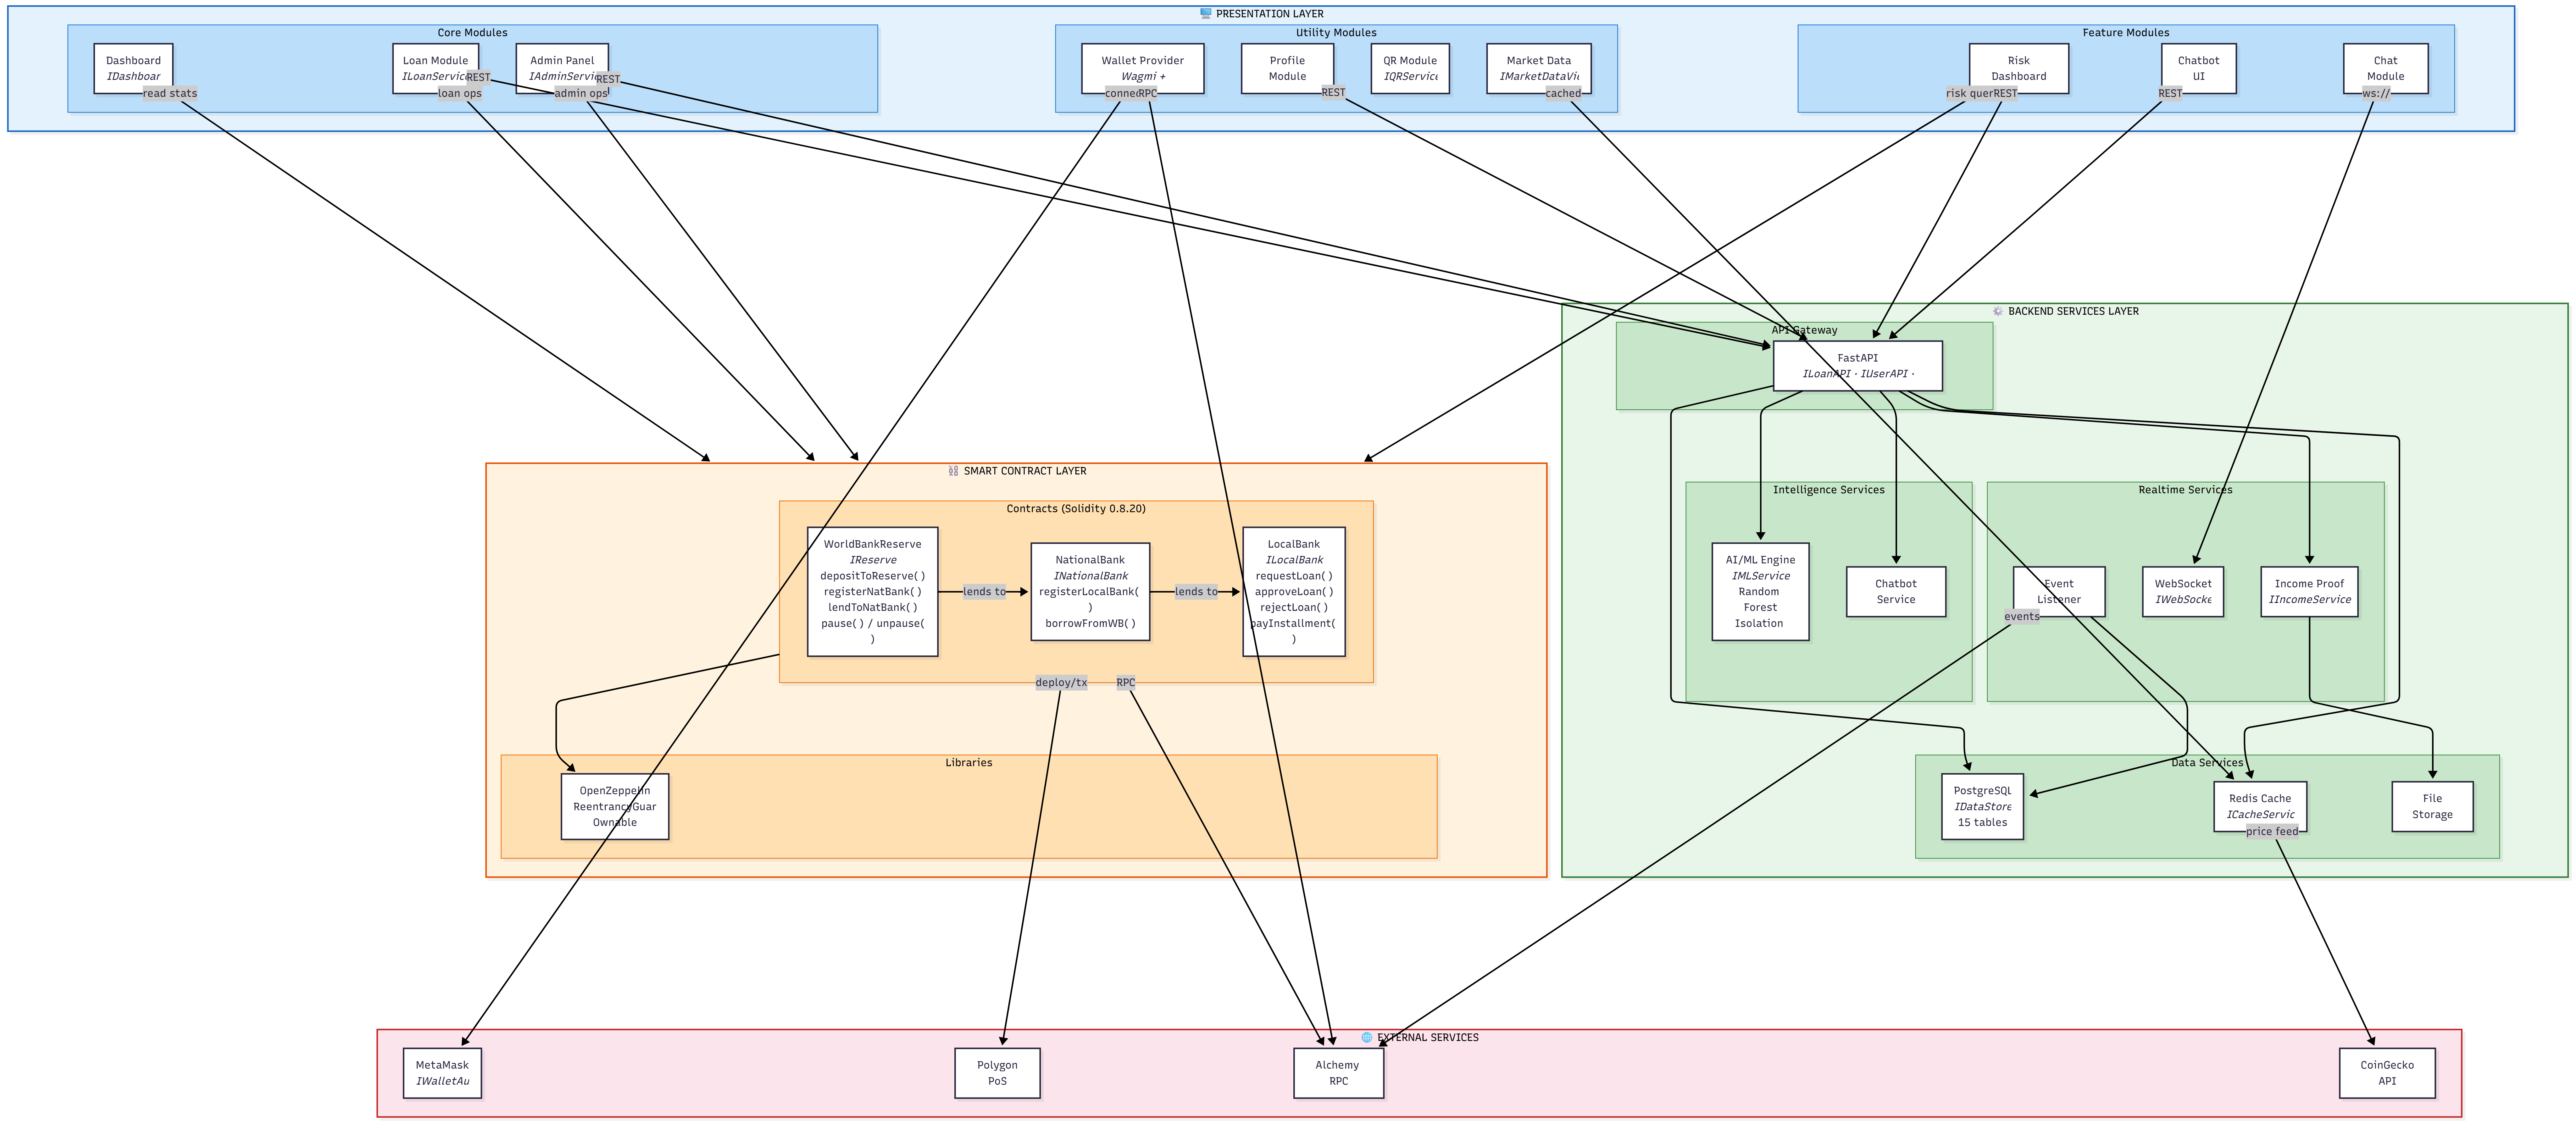
\includegraphics[width=\textwidth,keepaspectratio]{Component Diagram.png}
\caption{Component diagram showing interactions between the presentation layer, smart contract layer, off-chain backend services, and external systems.}
\label{fig:component-diagram}
\end{figure}

\section{Blockchain Platform Selection}

\begin{moderntable}
\caption{Blockchain platform selection criteria and justification.}
\begin{tabular}{@{} >{\raggedright}p{3cm} >{\raggedright}p{3.8cm} >{\raggedright\arraybackslash}p{5.2cm} @{}}
\toprule
\tableheadfont Criterion & \tableheadfont Selection & \tableheadfont Justification \\
\midrule
\rowcolor{RowShade}
Platform & Ethereum Virtual Machine (EVM) & Largest developer ecosystem; battle-tested security model; extensive tooling \\
Network & Polygon Mumbai / Ethereum Sepolia (testnets) & Zero-cost deployment; production-equivalent behavior; free faucet access \\
\rowcolor{RowShade}
Consensus & Proof-of-Stake (PoS) via Polygon validators & Energy-efficient; sub-2-second block finality; decentralized validator set \\
Smart contract language & Solidity 0.8.20 & Industry standard; mature compiler with overflow protection; rich library ecosystem \\
\bottomrule
\end{tabular}
\end{moderntable}

\subsection{Transaction Verification and Consensus}

\begin{itemize}[noitemsep]
\item \textbf{Polygon PoS:} Transactions are validated by a decentralized set of PoS validators. Block finality is achieved within approximately 2 seconds. Checkpoints are periodically committed to Ethereum mainnet for additional security.
\item \textbf{On prototype testnets:} Mumbai and Sepolia employ analogous consensus models with no financial cost, enabling iterative development and testing.
\end{itemize}


\section{Data Model and Database Design}

The relational database schema comprises 15 normalized entities in Third Normal Form (3NF). Figure~\ref{fig:core-system-graph} presents the core system graph showing entity relationships, Figure~\ref{fig:erd} presents the full Entity-Relationship Diagram (ERD), and Figure~\ref{fig:eer} presents the Enhanced Entity-Relationship (EER) diagram.

\begin{figure}[H]
\centering
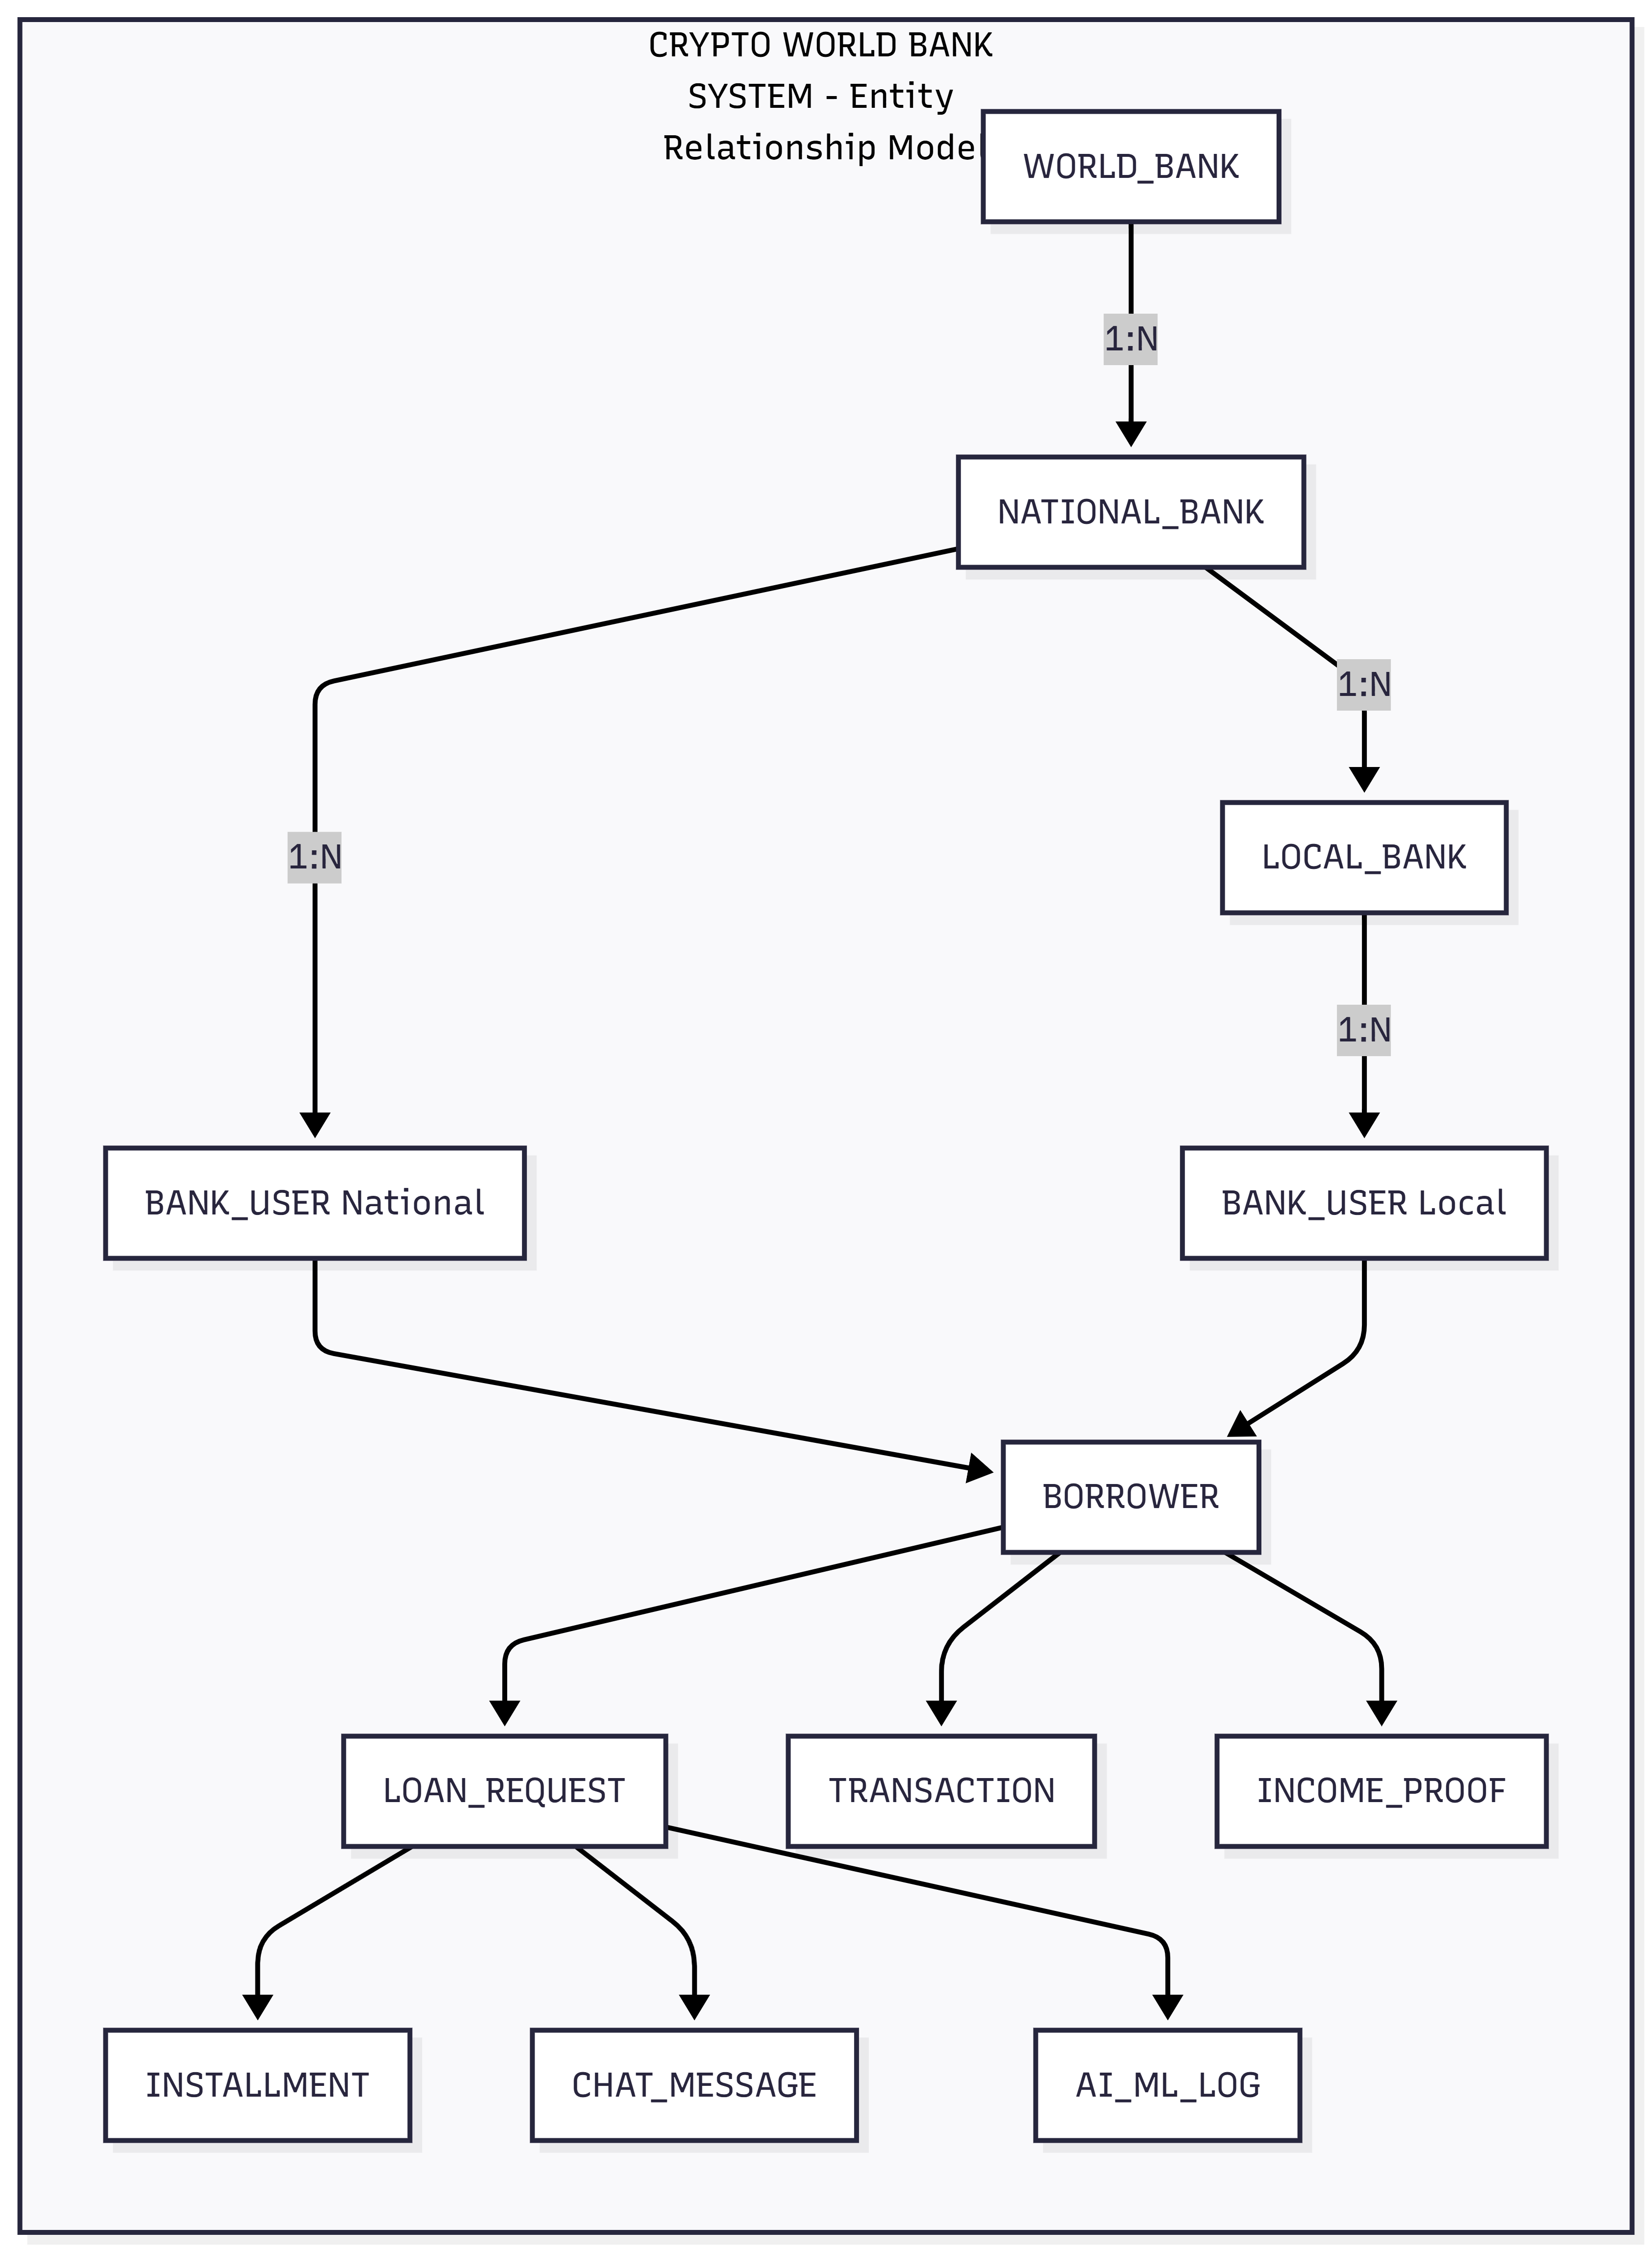
\includegraphics[width=\textwidth,keepaspectratio]{Core System Graph.png}
\caption{Core system graph showing the Crypto World Bank entity relationship model with hierarchical banking structure, lending lifecycle, communication, and security entities.}
\label{fig:core-system-graph}
\end{figure}

\begin{figure}[H]
\centering
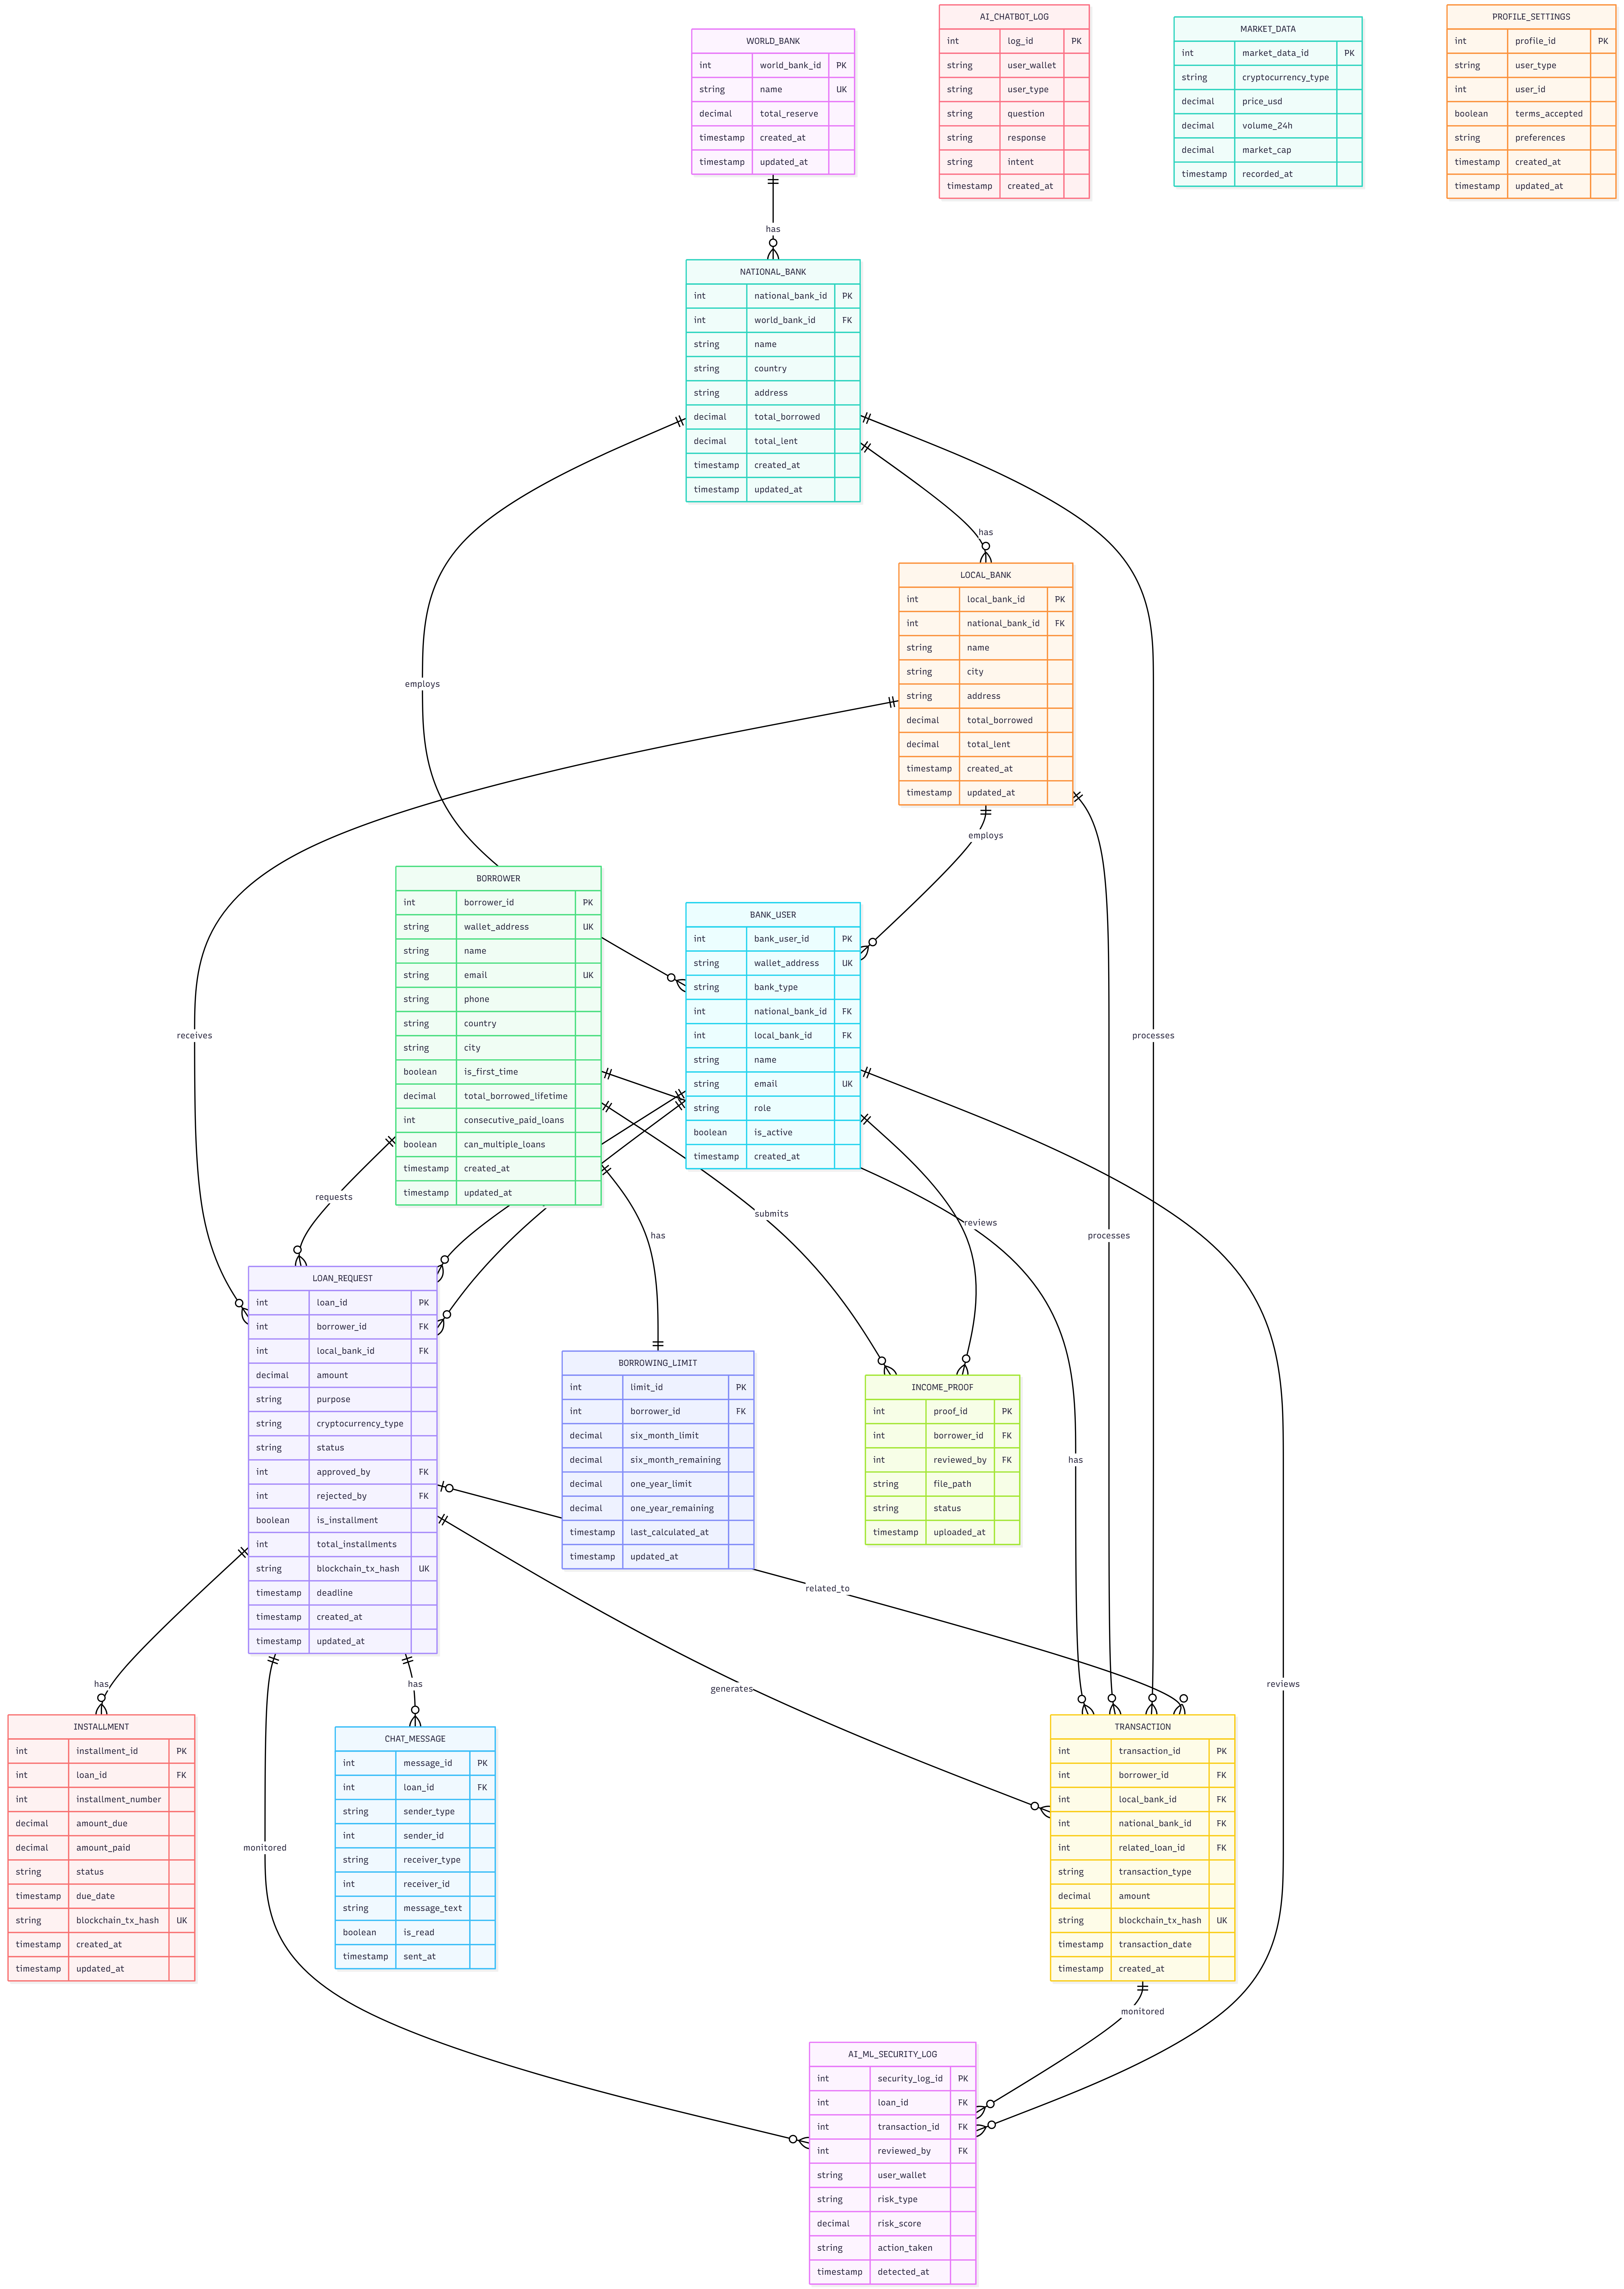
\includegraphics[width=\textwidth,keepaspectratio]{ERD diagram database management.png}
\caption{Entity-Relationship Diagram (ERD) for the Crypto World Bank database with relational symbols and entity attributes across all 15 tables.}
\label{fig:erd}
\end{figure}

\begin{figure}[H]
\centering
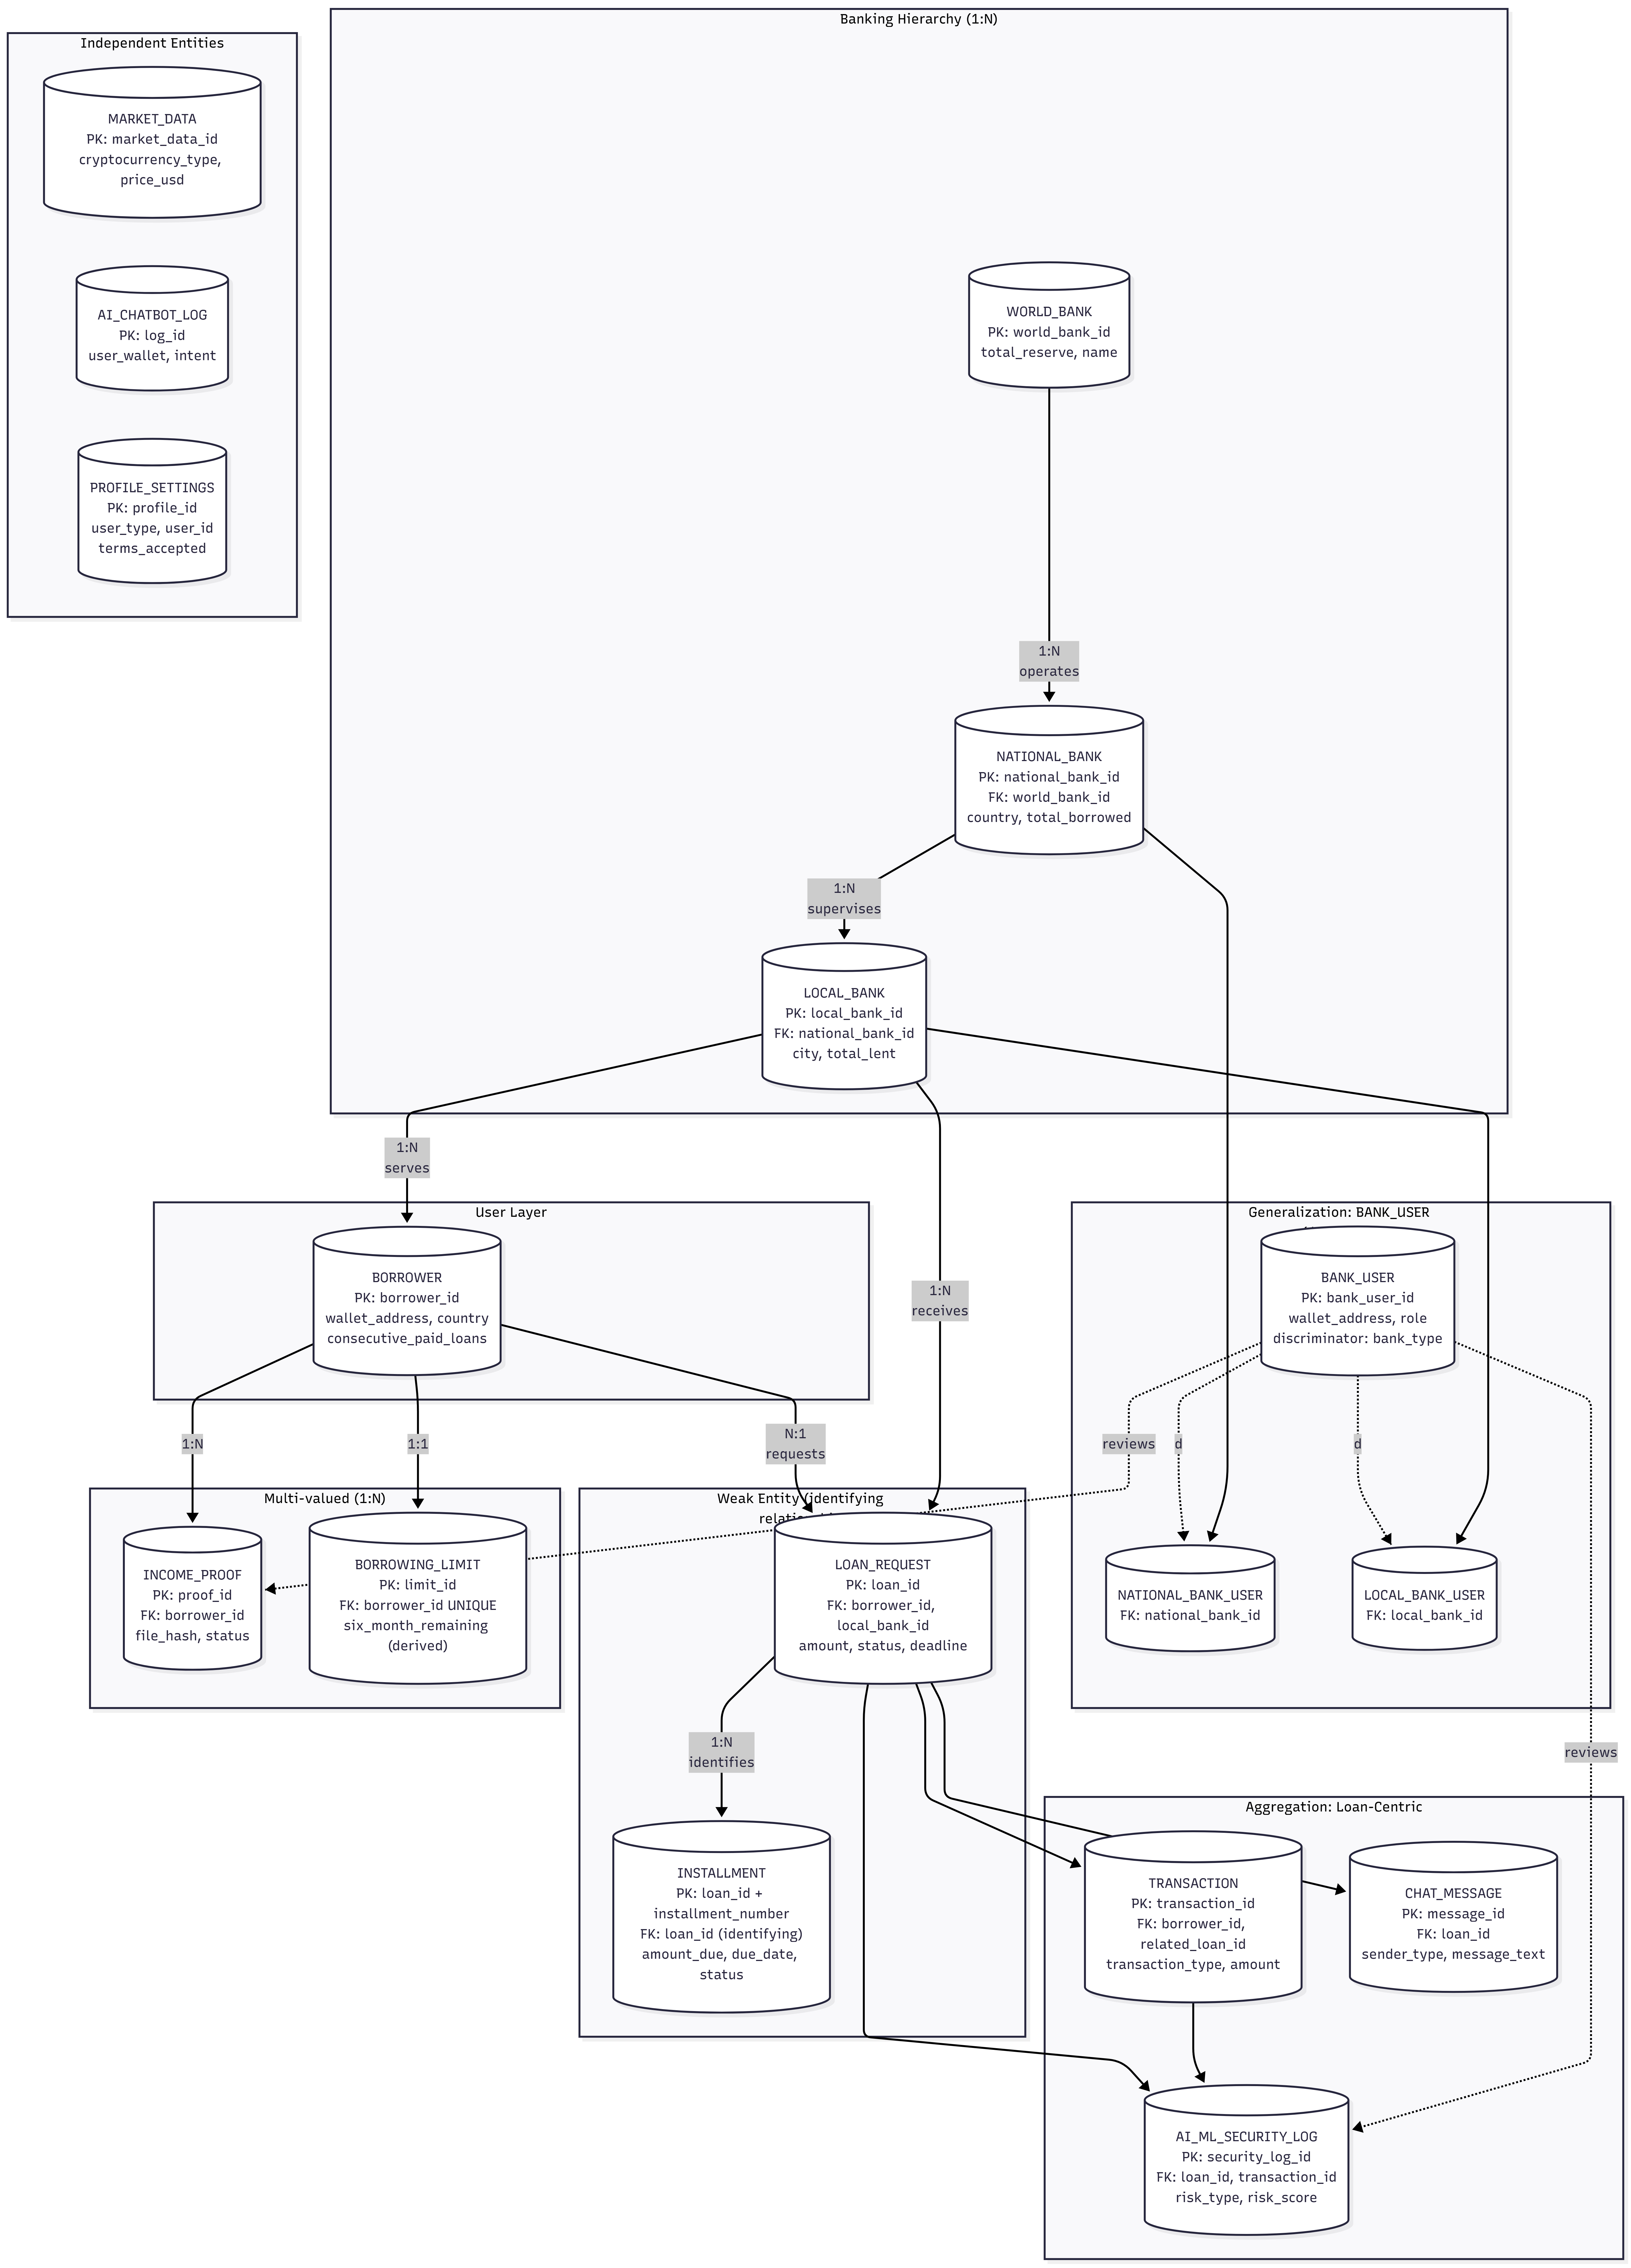
\includegraphics[width=\textwidth,keepaspectratio]{EER Diagram - Full Model.png}
\caption{Enhanced Entity-Relationship (EER) diagram showing generalization/specialization, weak entities, aggregation, participation constraints, and cardinality for the complete data model.}
\label{fig:eer}
\end{figure}

\subsection{Entity Summary}

\begin{moderntable}
\caption{Database entity summary (15 entities).}
\begin{tabular}{@{} >{\raggedright}p{3.5cm} >{\raggedright\arraybackslash}p{8.5cm} @{}}
\toprule
\tableheadfont Entity & \tableheadfont Role \\
\midrule
\rowcolor{RowShade}
WORLD\_BANK & Top-level reserve holder; global lending parameters \\
NATIONAL\_BANK & Country-level banks; borrow from World Bank \\
\rowcolor{RowShade}
LOCAL\_BANK & City-level banks; retail lending to borrowers \\
BANK\_USER & Bank staff with role-based permissions (approve/reject loans) \\
\rowcolor{RowShade}
BORROWER & End-users requesting and repaying loans \\
LOAN\_REQUEST & Loan applications and full lifecycle tracking \\
\rowcolor{RowShade}
INSTALLMENT & Installment payment records (weak entity dependent on LOAN\_REQUEST) \\
TRANSACTION & Financial transaction records \\
\rowcolor{RowShade}
BORROWING\_LIMIT & Per-borrower limits with derived 6-month/1-year windows \\
INCOME\_PROOF & Income verification documents (multi-valued per borrower) \\
\rowcolor{RowShade}
CHAT\_MESSAGE & Borrower--bank communication \\
AI\_CHATBOT\_LOG & AI chatbot interaction records \\
\rowcolor{RowShade}
AI\_ML\_SECURITY\_LOG & Security and ML monitoring events \\
MARKET\_DATA & Cryptocurrency price feeds \\
\rowcolor{RowShade}
PROFILE\_SETTINGS & User profile and platform preferences \\
\bottomrule
\end{tabular}
\end{moderntable}

\subsection{EER Constructs Applied}

\begin{moderntable}
\caption{EER constructs applied in the Crypto World Bank data model.}
\begin{tabular}{@{} >{\raggedright}p{3.2cm} >{\raggedright\arraybackslash}p{9cm} @{}}
\toprule
\tableheadfont EER Construct & \tableheadfont Application \\
\midrule
\rowcolor{RowShade}
Generalization (disjoint) & BANK\_USER generalizes to NATIONAL\_BANK\_USER and LOCAL\_BANK\_USER via \texttt{bank\_type} discriminator with mutually exclusive foreign keys \\
Weak entity & INSTALLMENT is existence-dependent on LOAN\_REQUEST with partial key \texttt{installment\_number} \\
\rowcolor{RowShade}
Aggregation & LOAN\_REQUEST aggregates BORROWER + LOCAL\_BANK; TRANSACTION, CHAT\_MESSAGE, and AI\_ML\_SECURITY\_LOG are components \\
Multi-valued attribute & INCOME\_PROOF modeled as a separate entity (borrower can have multiple proofs) \\
\rowcolor{RowShade}
Derived attribute & \texttt{six\_month\_remaining} and \texttt{one\_year\_remaining} in BORROWING\_LIMIT are computed from TRANSACTION history \\
Composite key & INSTALLMENT uses (\texttt{loan\_id}, \texttt{installment\_number}) \\
\rowcolor{RowShade}
Participation constraints & BORROWER has total participation in LOAN\_REQUEST; INSTALLMENT has total participation when \texttt{is\_installment = TRUE} \\
Cardinality & 1:1 (BORROWER--BORROWING\_LIMIT), 1:N (hierarchy, loan--installment), N:1 (loan--borrower) \\
\bottomrule
\end{tabular}
\end{moderntable}

\subsection{Normalization}

The schema is normalized to Third Normal Form (3NF) with verification against Boyce-Codd Normal Form (BCNF):

\begin{itemize}[noitemsep]
\item \textbf{1NF:} All attributes are atomic with no repeating groups. Multi-valued attributes like income proofs are stored in separate entities.
\item \textbf{2NF:} No partial dependencies exist. INSTALLMENT's non-key attributes depend on the full composite key (\texttt{loan\_id}, \texttt{installment\_number}).
\item \textbf{3NF:} No transitive dependencies. Derived values such as \texttt{total\_borrowed} in bank entities are computed at query time rather than stored redundantly.
\item \textbf{BCNF:} All determinants are candidate keys. A CHECK constraint on BANK\_USER enforces disjoint specialization of the generalization hierarchy.
\end{itemize}

\subsection{Indexing Strategy}

We use B-tree indexes (the default in PostgreSQL) for efficient retrieval on frequently queried columns:

\begin{moderntable}
\caption{Database indexing strategy.}
\begin{tabular}{@{} >{\raggedright}p{3cm} >{\raggedright}p{4.5cm} >{\raggedright\arraybackslash}p{4.5cm} @{}}
\toprule
\tableheadfont Table & \tableheadfont Index & \tableheadfont Purpose \\
\midrule
\rowcolor{RowShade}
LOAN\_REQUEST & \texttt{idx\_status\_borrower}, \texttt{idx\_status\_bank}, \texttt{idx\_deadline} & Filter pending loans; lookup by borrower or bank \\
TRANSACTION & \texttt{idx\_type\_date}, \texttt{idx\_borrower\_date}, \texttt{idx\_date} & Borrowing limit queries (6-month/1-year windows) \\
\rowcolor{RowShade}
BORROWER & \texttt{idx\_wallet}, \texttt{idx\_location} & Wallet address lookup; location-based queries \\
CHAT\_MESSAGE & \texttt{idx\_loan\_sent}, \texttt{idx\_sender}, \texttt{idx\_receiver} & Chat history retrieval; unread message counts \\
\bottomrule
\end{tabular}
\end{moderntable}

B-tree indexes are chosen for their efficiency with range queries (e.g., transactions within the last 6 months); hash indexes would be suitable only for exact-match lookups.

\subsection{Functional Dependencies}

\begin{moderntable}
\caption{Representative functional dependencies.}
\begin{tabular}{@{} >{\raggedright}p{3cm} >{\raggedright}p{5cm} >{\raggedright\arraybackslash}p{4cm} @{}}
\toprule
\tableheadfont Relation & \tableheadfont Functional Dependency & \tableheadfont Notes \\
\midrule
\rowcolor{RowShade}
LOAN\_REQUEST & \texttt{loan\_id} $\to$ all attributes & Primary key determines row \\
LOAN\_REQUEST & \texttt{borrower\_id, local\_bank\_id} $\to$ \texttt{status, amount}, \ldots & One active request per borrower per bank \\
\rowcolor{RowShade}
BORROWING\_LIMIT & \texttt{borrower\_id} $\to$ \texttt{six\_month\_limit, one\_year\_limit}, \ldots & 1:1 with BORROWER \\
\bottomrule
\end{tabular}
\end{moderntable}

\subsection{Relational Integrity Constraints}

\begin{moderntable}
\caption{Relational integrity constraints.}
\begin{tabular}{@{} >{\raggedright}p{2.5cm} >{\raggedright\arraybackslash}p{9.5cm} @{}}
\toprule
\tableheadfont Constraint Type & \tableheadfont Examples \\
\midrule
\rowcolor{RowShade}
Primary Key & \texttt{world\_bank\_id}, \texttt{loan\_id}, \texttt{borrower\_id}, etc. \\
Foreign Key & \texttt{local\_bank\_id} in LOAN\_REQUEST references LOCAL\_BANK \\
\rowcolor{RowShade}
UNIQUE & \texttt{wallet\_address} in BORROWER; \texttt{blockchain\_tx\_hash} in LOAN\_REQUEST \\
CHECK & BANK\_USER: \texttt{(bank\_type='national' AND national\_bank\_id IS NOT NULL) OR (bank\_type='local' AND local\_bank\_id IS NOT NULL)} \\
\rowcolor{RowShade}
NOT NULL & Core attributes: \texttt{name}, \texttt{wallet\_address}, \texttt{status} \\
\bottomrule
\end{tabular}
\end{moderntable}


\section{On-Chain and Off-Chain Data Partitioning}

\begin{moderntable}
\caption{Data partitioning between on-chain and off-chain storage.}
\begin{tabular}{@{} >{\raggedright}p{4.2cm} >{\raggedright}p{2.5cm} >{\raggedright\arraybackslash}p{5.3cm} @{}}
\toprule
\tableheadfont Data Category & \tableheadfont Storage & \tableheadfont Rationale \\
\midrule
\rowcolor{RowShade}
Reserve balances, loan requests, approval/rejection events, repayment transactions & On-chain & Immutability, public auditability, trustless verification \\
User profiles, income verification documents, chat messages, AI/ML inference logs & Off-chain (PostgreSQL) & Data privacy, query flexibility, storage cost optimization \\
\rowcolor{RowShade}
Borrowing limit computations & Off-chain with on-chain enforcement & Complex temporal aggregation; results committed as on-chain constraints \\
Cryptocurrency market data & Off-chain (cached) & High-frequency updates; external API dependency \\
\bottomrule
\end{tabular}
\end{moderntable}


\section{Digital Identity System}

\begin{itemize}[noitemsep]
\item \textbf{Wallet-based identity:} Users authenticate via Ethereum wallet signatures (MetaMask, WalletConnect). No centralized credential store is required.
\item \textbf{Role binding:} Wallet addresses are mapped to hierarchical roles (Owner, National Bank, Local Bank, Approver, Borrower) within the smart contract permission system.
\end{itemize}


\section{System Modeling}

This section presents the system analysis diagrams that model the platform's structure, behavior, and data flow.

\subsection{Use Case Diagram}

The system involves four primary actors---Borrower, Bank Approver, World Bank Admin, and National Bank---across 29 use cases. Figure~\ref{fig:usecase} shows the complete use case diagram.

\begin{figure}[H]
\centering
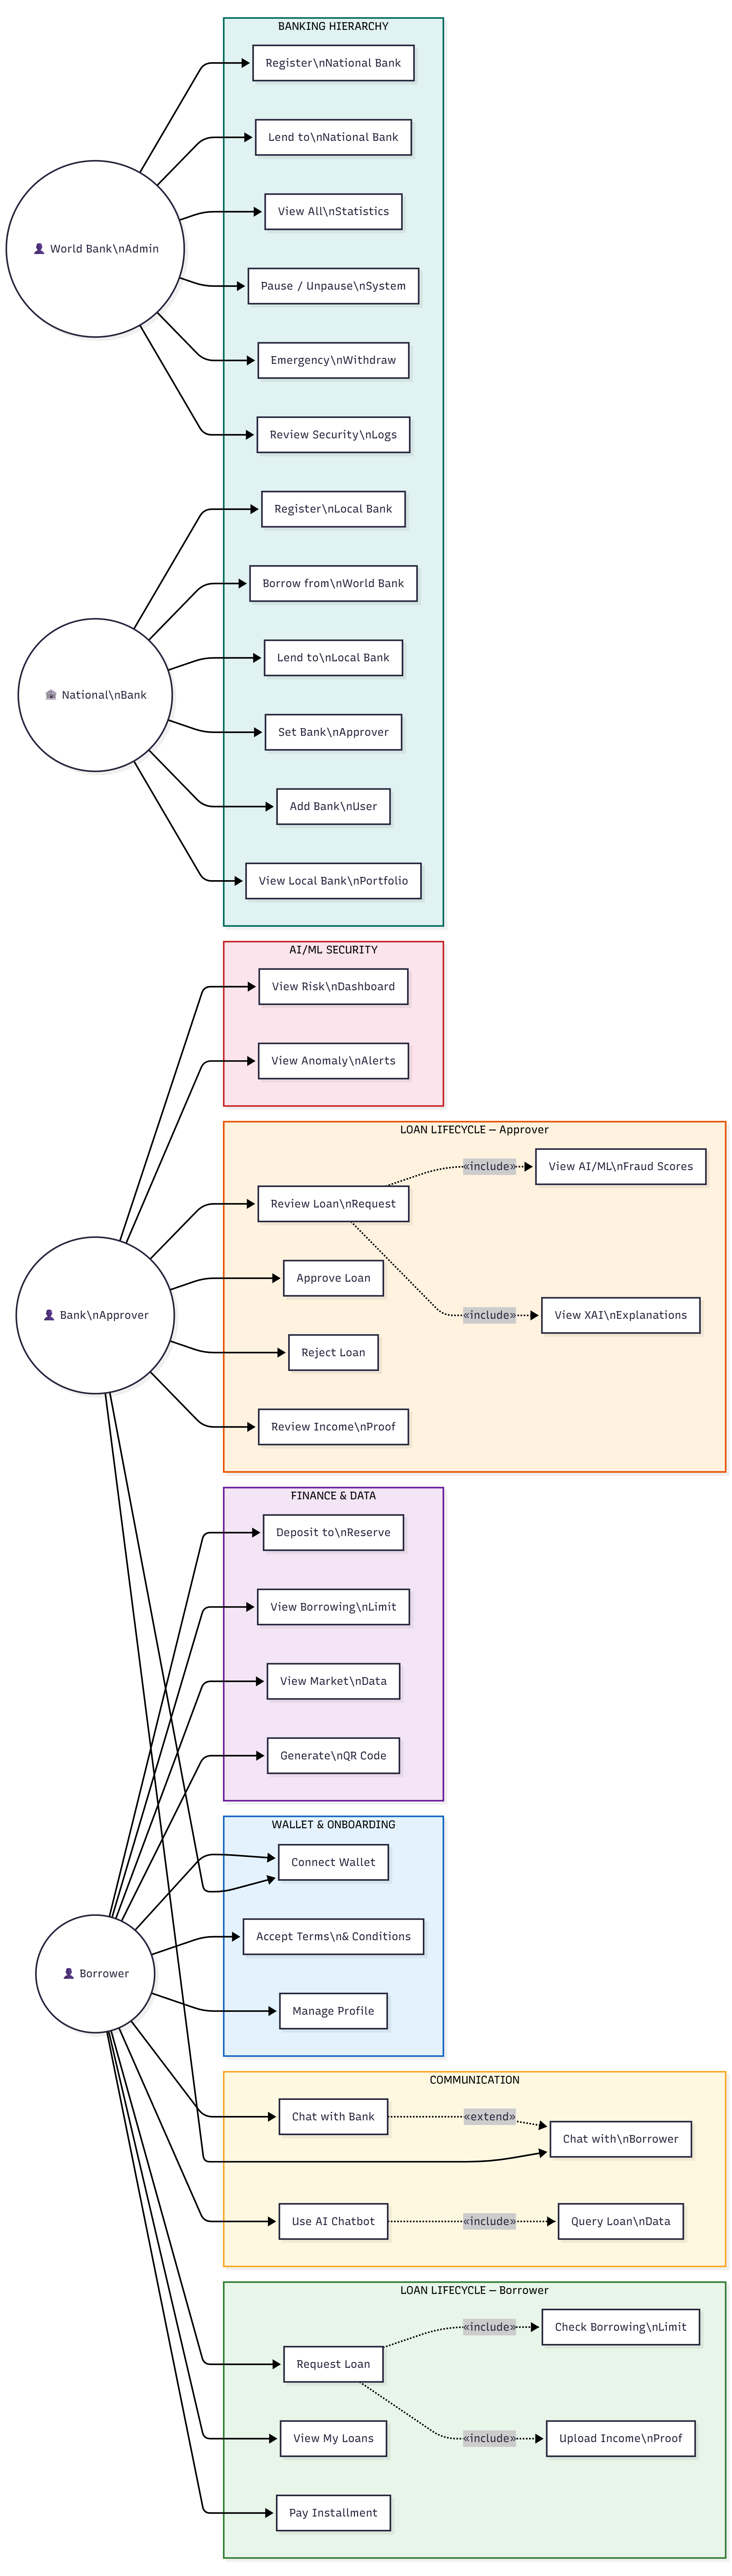
\includegraphics[width=\textwidth,keepaspectratio]{Usecase diagram.png}
\caption{Use case diagram showing 29 use cases across four actors: Borrower, Bank Approver, World Bank Admin, and National Bank.}
\label{fig:usecase}
\end{figure}

\subsection{Activity Diagrams}

Figures~\ref{fig:act-loan}--\ref{fig:act-profile} present the activity diagrams for the platform's seven core operational flows.

\begin{figure}[H]
\centering
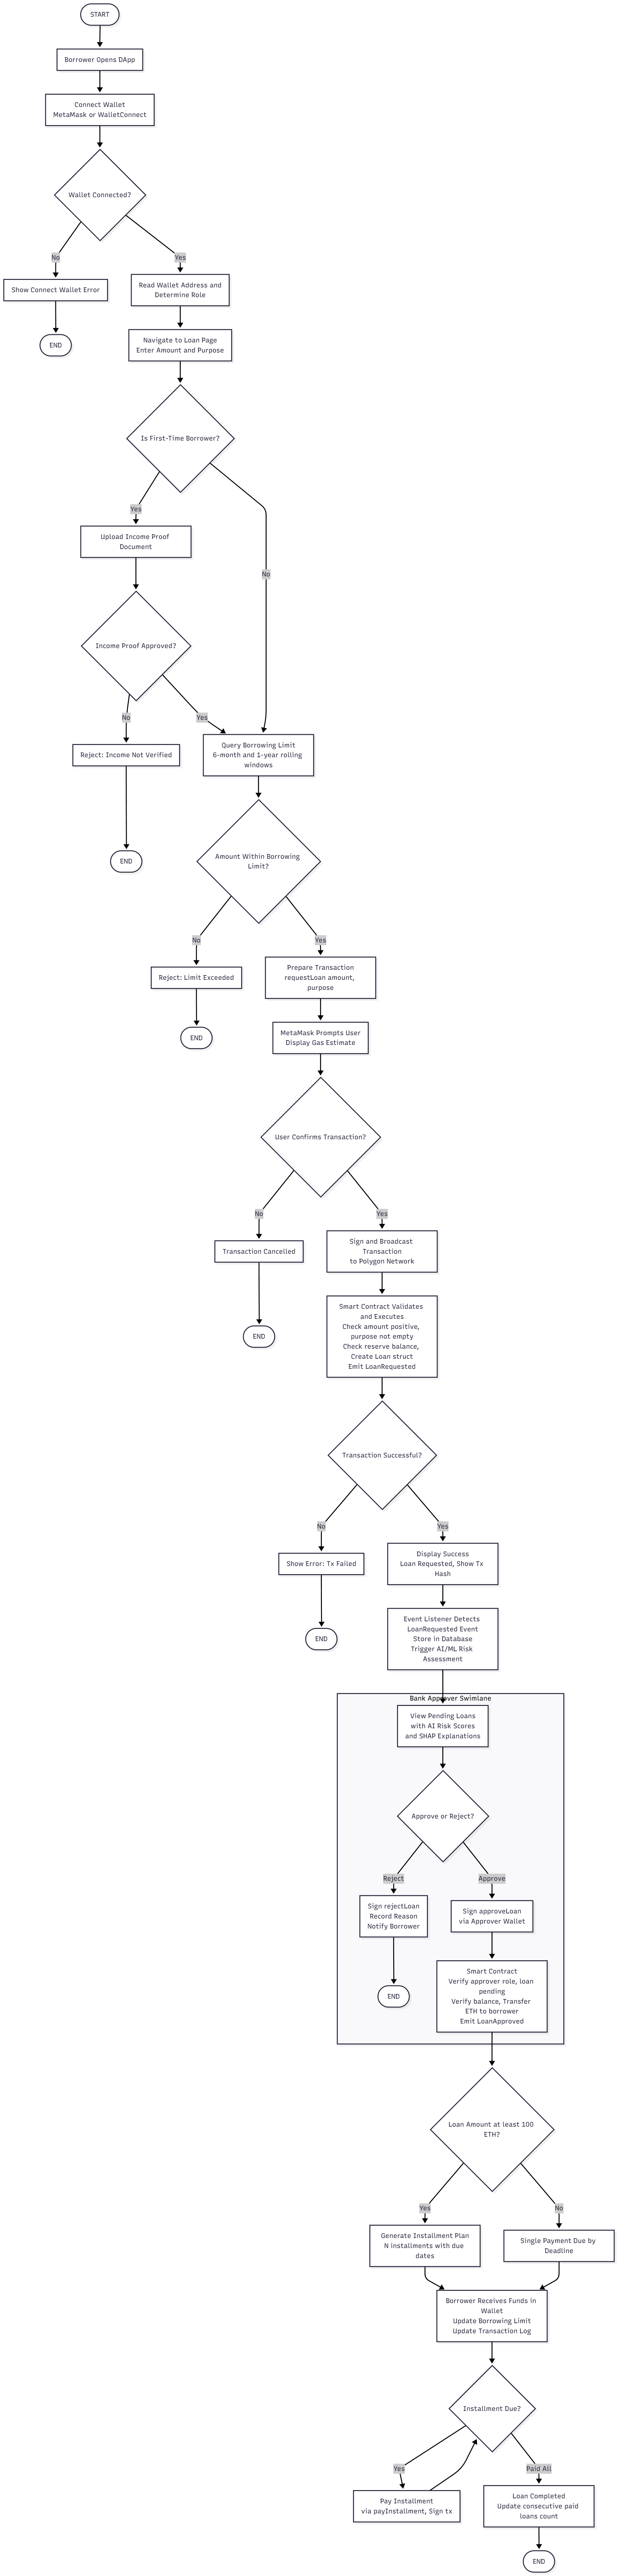
\includegraphics[width=0.92\textwidth,keepaspectratio]{Activity Diagram - Loan Request to Repayment Flow.png}
\caption{Activity diagram: Loan request to repayment flow, covering submission, AI risk assessment, approval/rejection, disbursement, and installment repayment.}
\label{fig:act-loan}
\end{figure}

\begin{figure}[H]
\centering
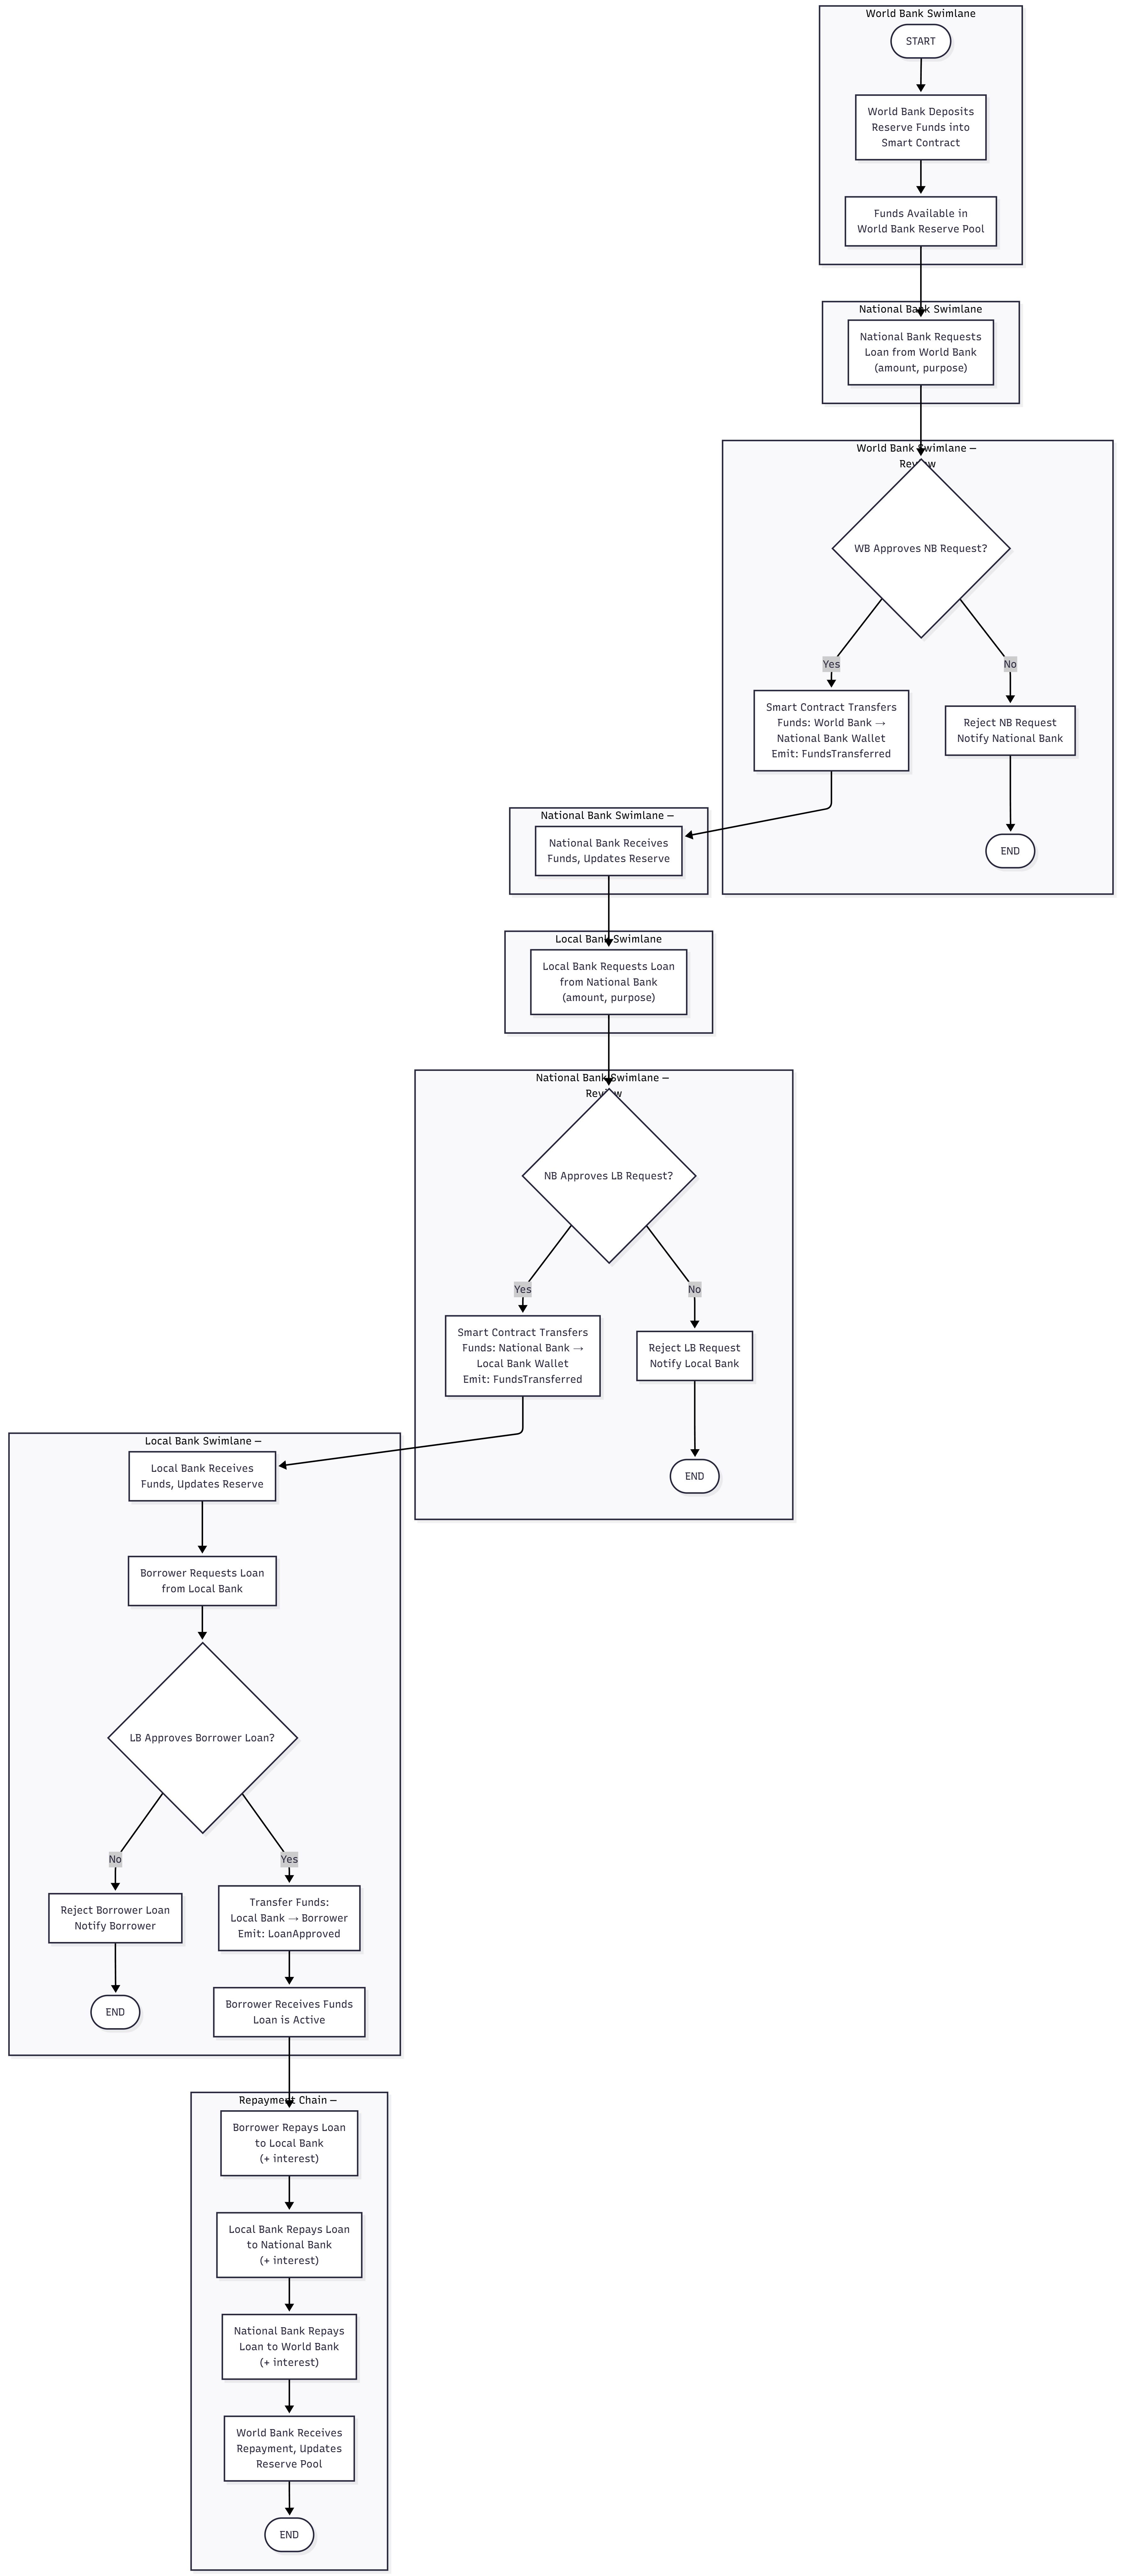
\includegraphics[width=0.92\textwidth,keepaspectratio]{Activity Diagram Hierarchical Banking Flow.png}
\caption{Activity diagram: Hierarchical banking flow showing capital distribution from World Bank through National Banks to Local Banks.}
\label{fig:act-hierarchy}
\end{figure}

\begin{figure}[H]
\centering
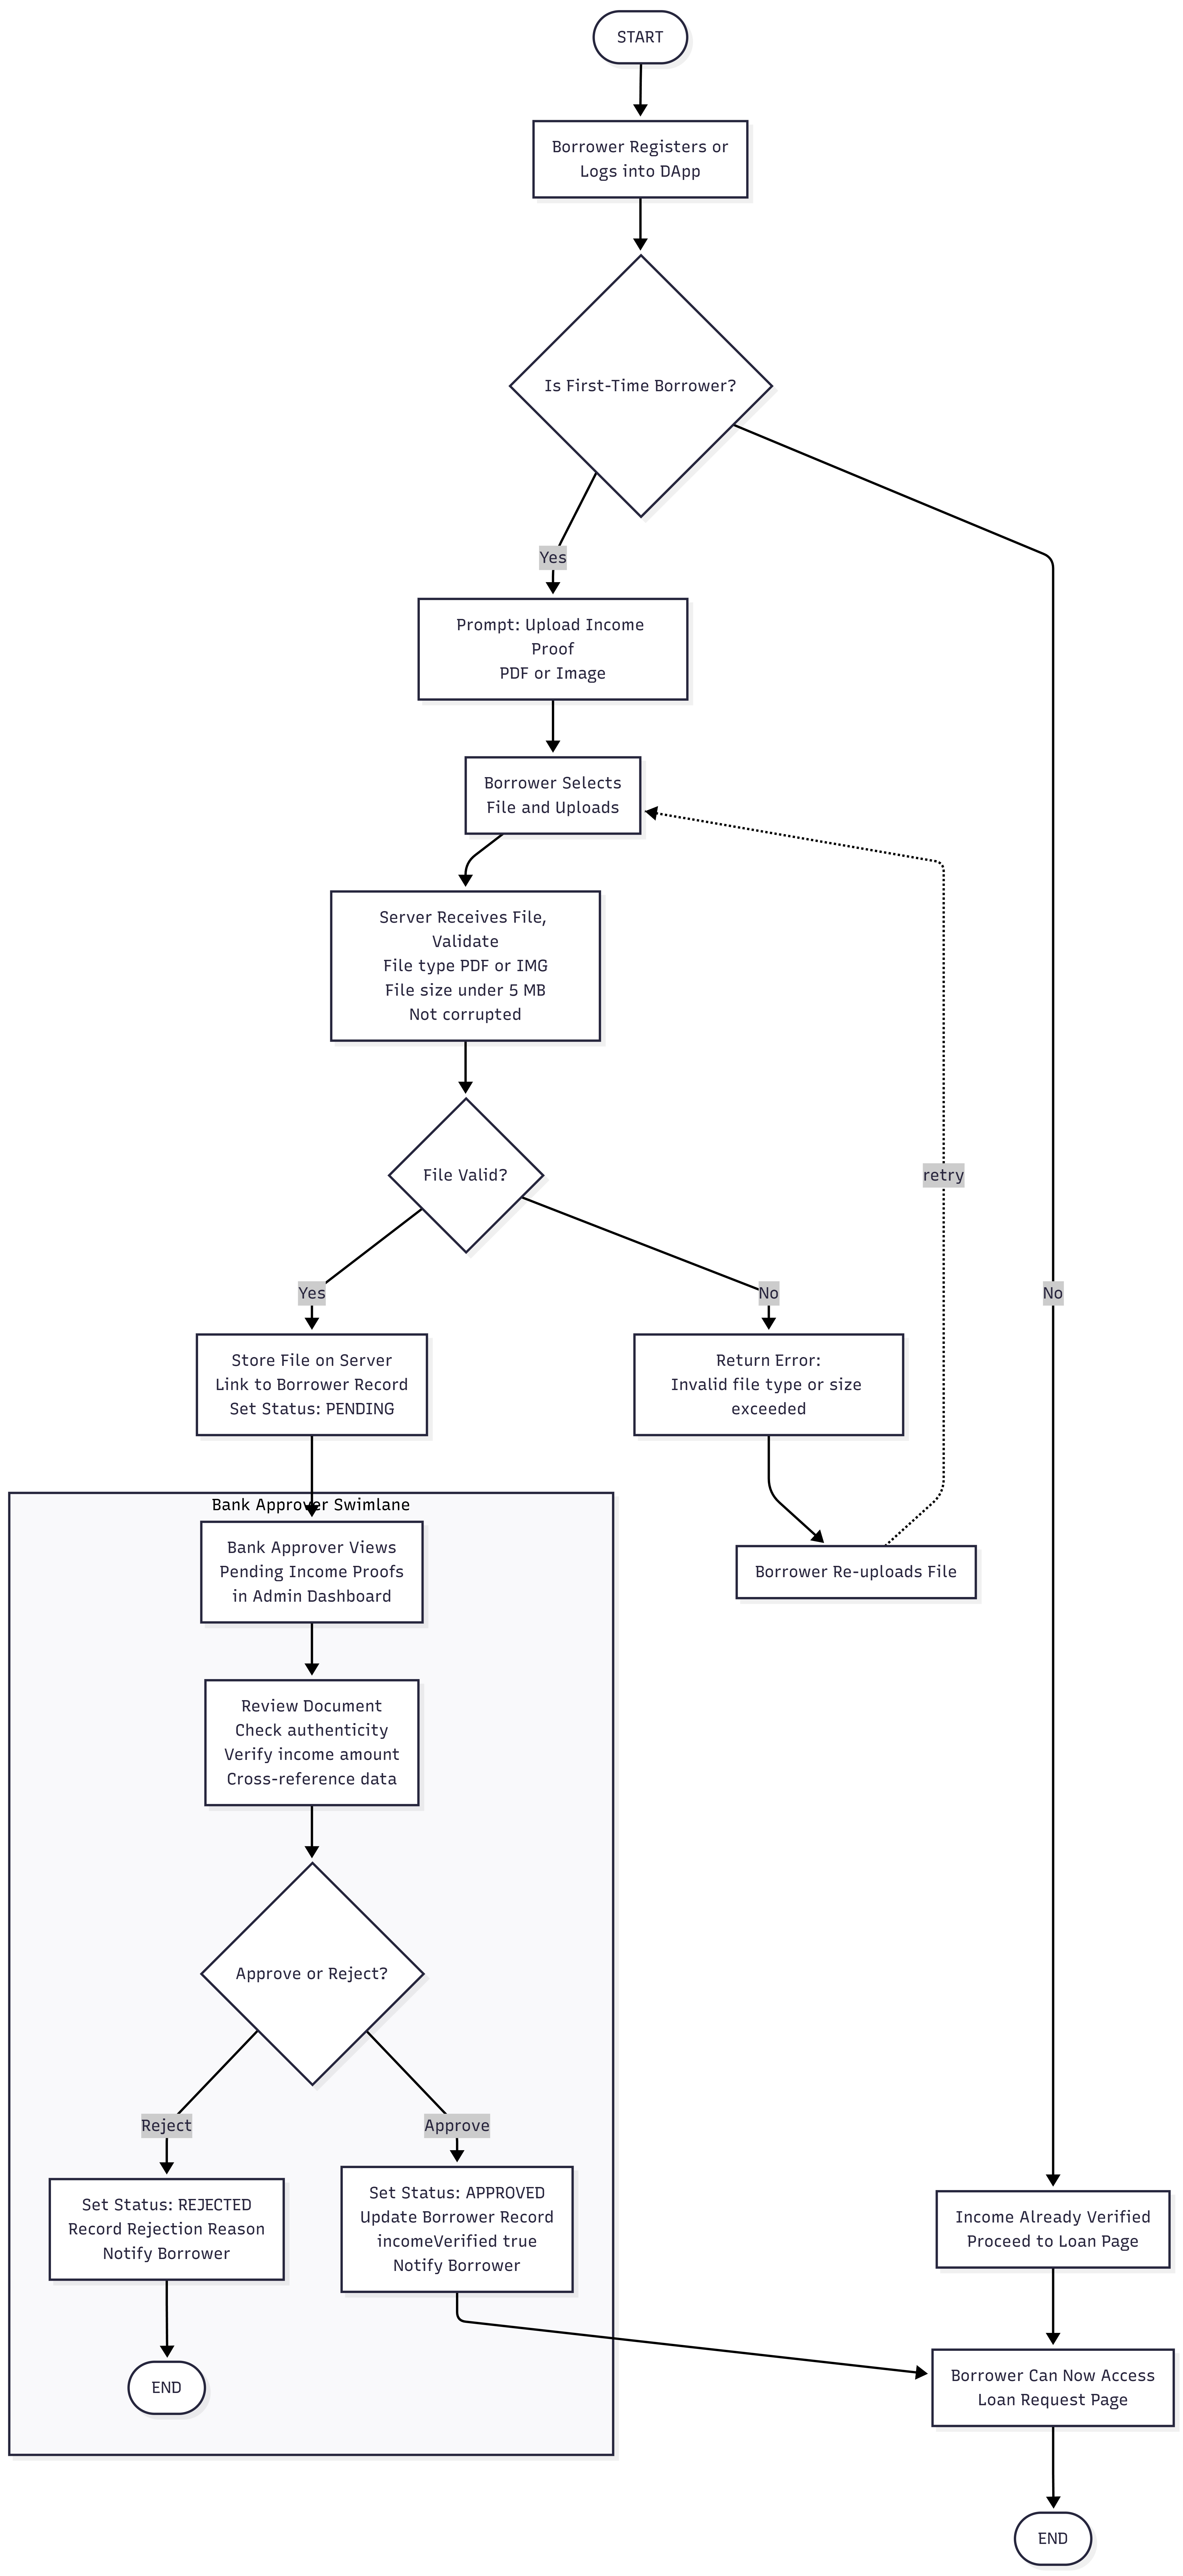
\includegraphics[width=0.85\textwidth,keepaspectratio]{Activity Diagram Income Verification Flow.png}
\caption{Activity diagram: Income verification flow for borrower document submission and bank officer review.}
\label{fig:act-income}
\end{figure}

\begin{figure}[H]
\centering
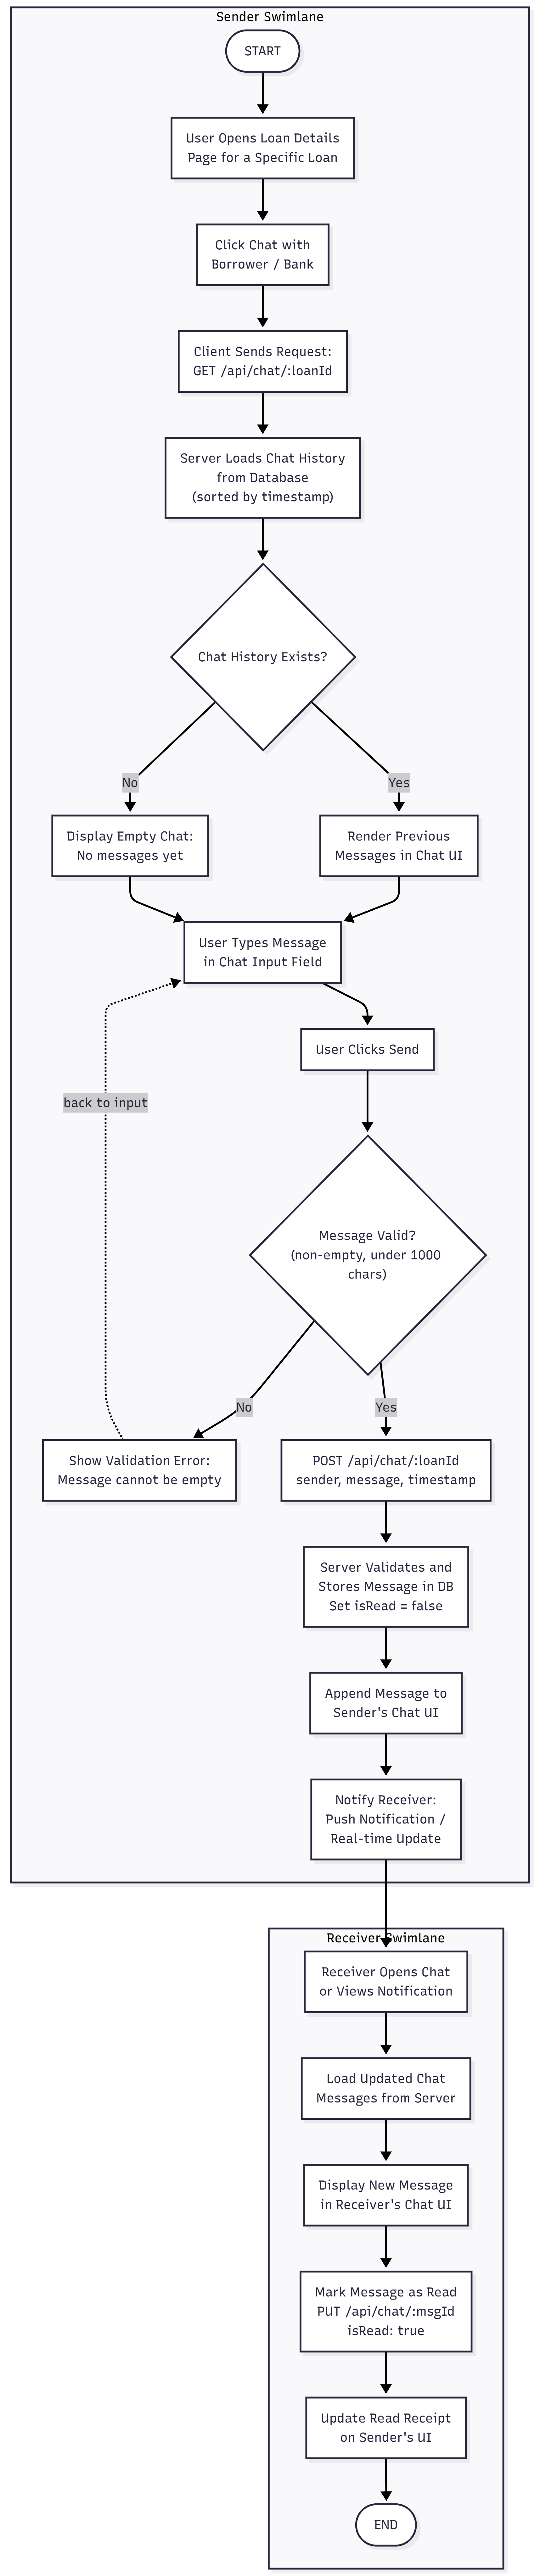
\includegraphics[width=0.85\textwidth,keepaspectratio]{Activity Diagram Chat System Flow.png}
\caption{Activity diagram: Chat system flow between borrowers and bank representatives during loan processing.}
\label{fig:act-chat}
\end{figure}

\begin{figure}[H]
\centering
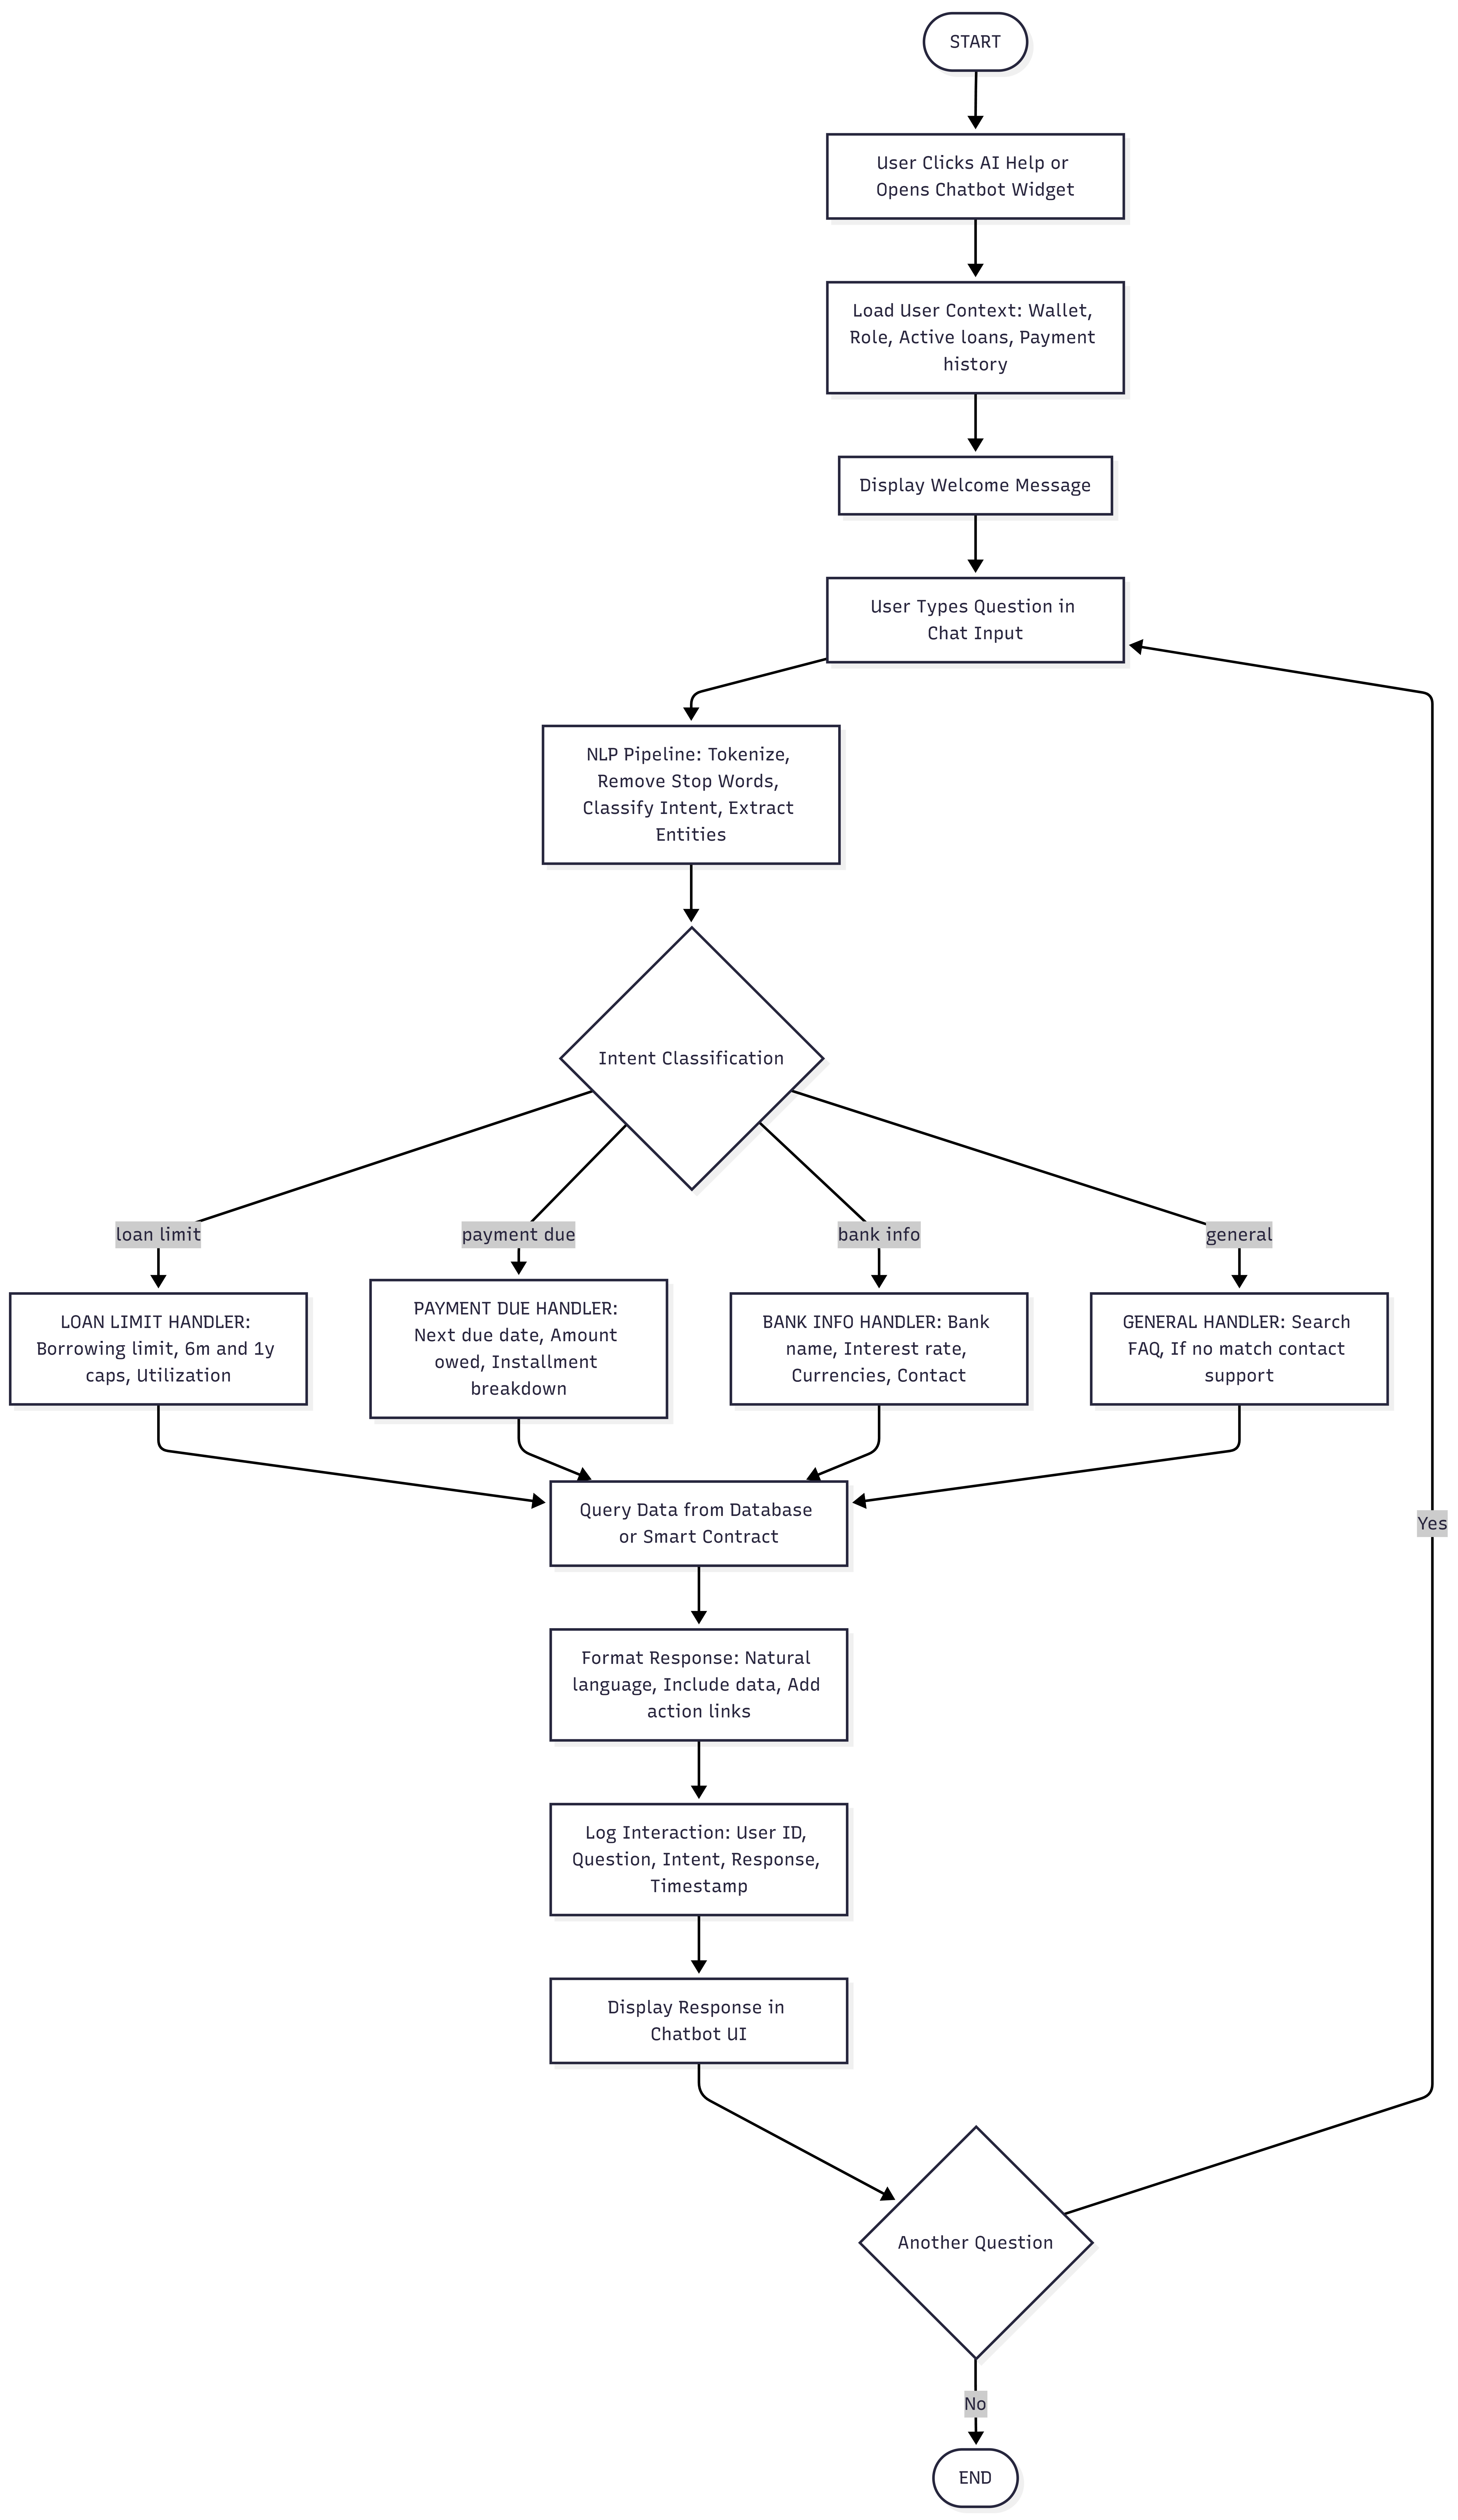
\includegraphics[width=0.85\textwidth,keepaspectratio]{Activity Diagram AI Chatbot Interaction Flow.png}
\caption{Activity diagram: AI chatbot interaction flow for automated borrower assistance and FAQ handling.}
\label{fig:act-aichatbot}
\end{figure}

\begin{figure}[H]
\centering
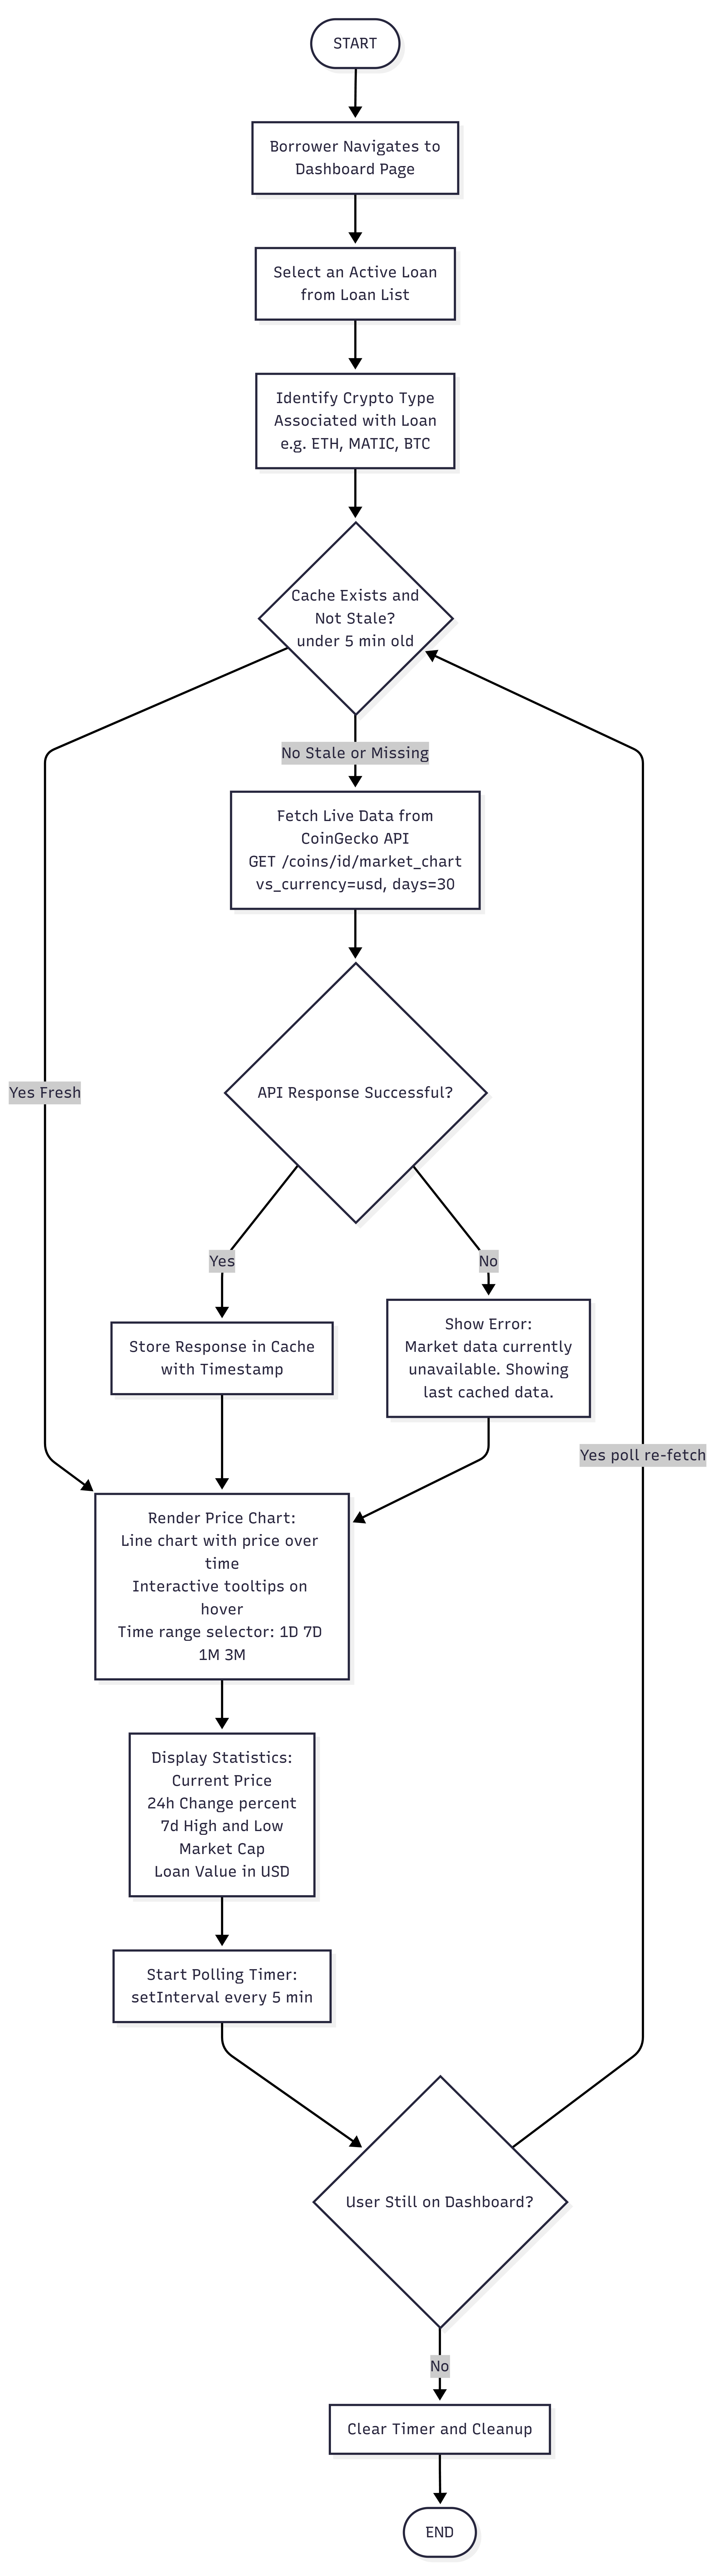
\includegraphics[width=0.85\textwidth,keepaspectratio]{activity diagram Market Data Viewing Flow.png}
\caption{Activity diagram: Market data viewing flow for cryptocurrency price visualization and trend analysis.}
\label{fig:act-market}
\end{figure}

\begin{figure}[H]
\centering
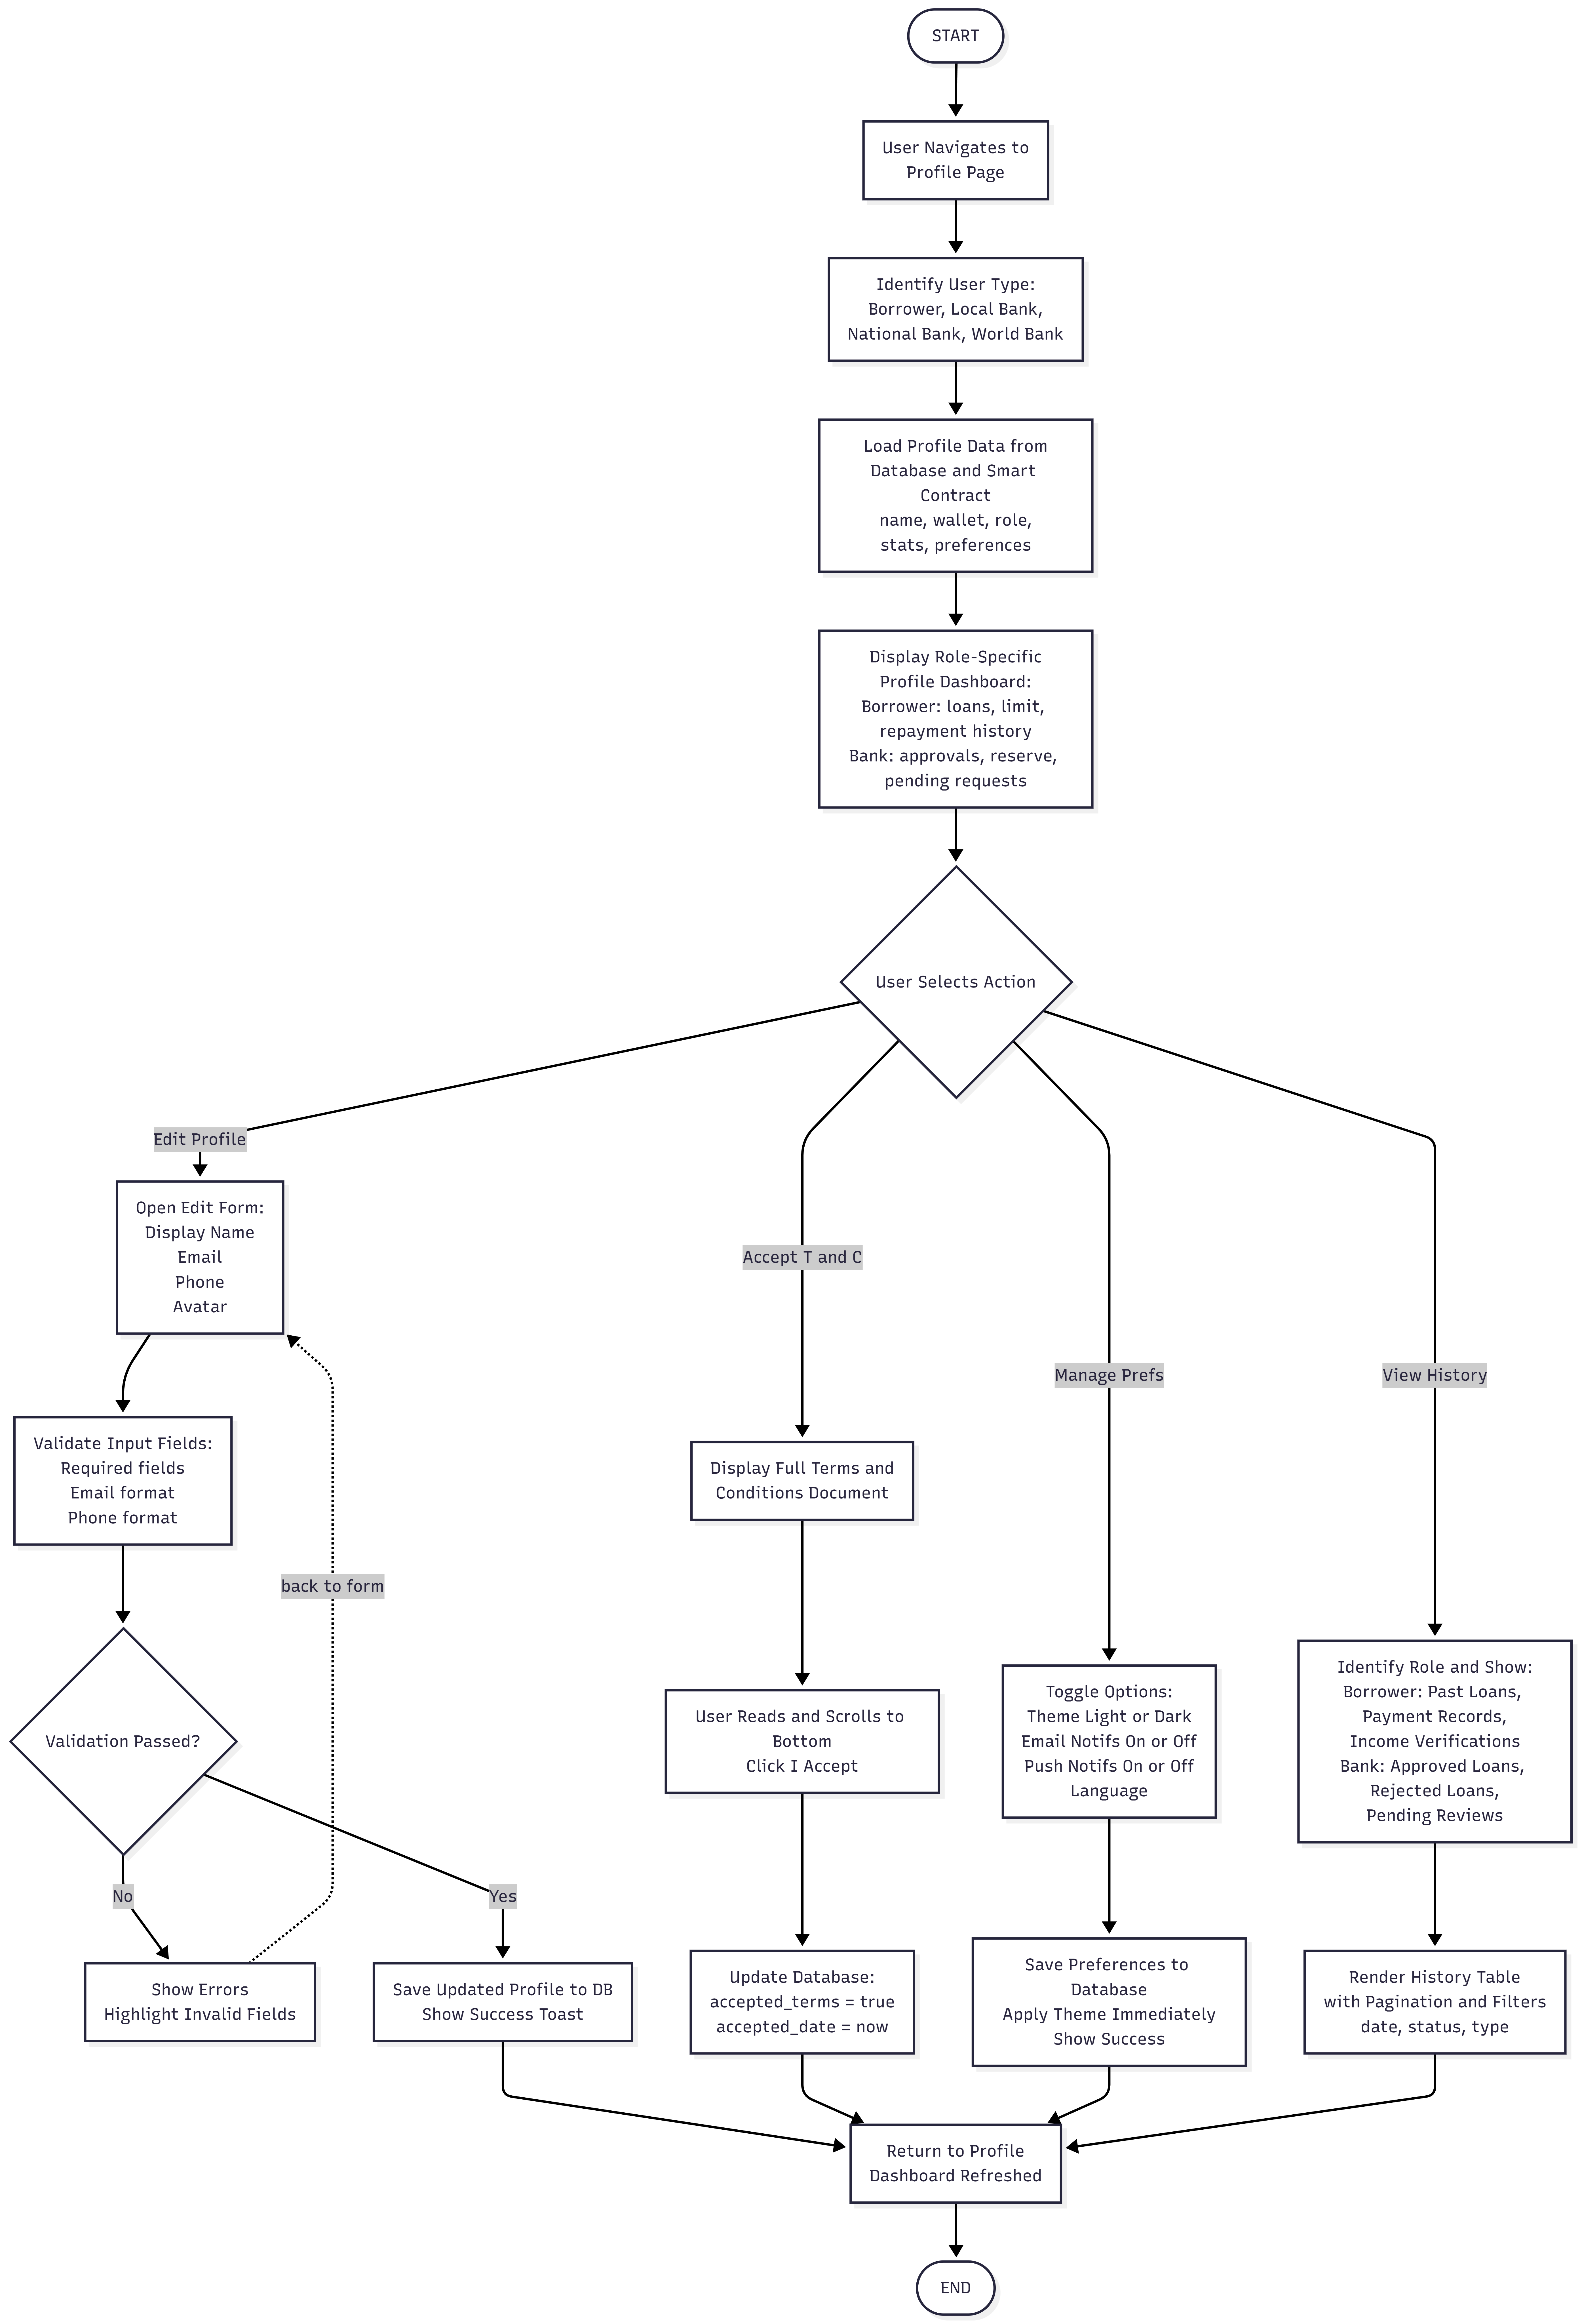
\includegraphics[width=0.85\textwidth,keepaspectratio]{Activity Diagram Profile Management Flow.png}
\caption{Activity diagram: Profile management flow for user settings, terms acceptance, and account configuration.}
\label{fig:act-profile}
\end{figure}

\subsection{Data Flow Diagrams}

Figures~\ref{fig:dfd-context}--\ref{fig:dfd-level1b} present the data flow diagrams at the context level (Level~0) and decomposed level (Level~1).

\begin{figure}[H]
\centering
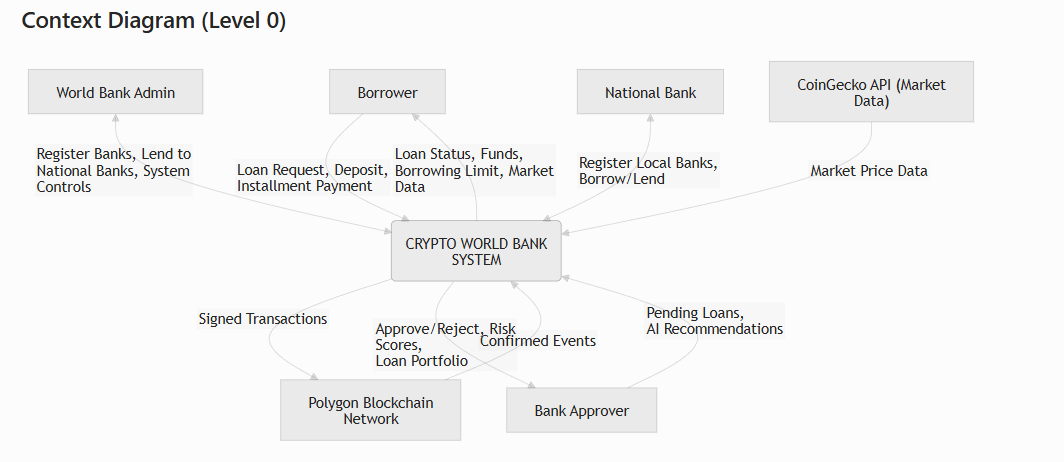
\includegraphics[width=\textwidth,keepaspectratio]{Dataflow Diagram (Context Diagram Level - 0).png}
\caption{Data flow diagram --- Context diagram (Level~0) showing external entities and data flows into and out of the Crypto World Bank system.}
\label{fig:dfd-context}
\end{figure}

\begin{figure}[H]
\centering
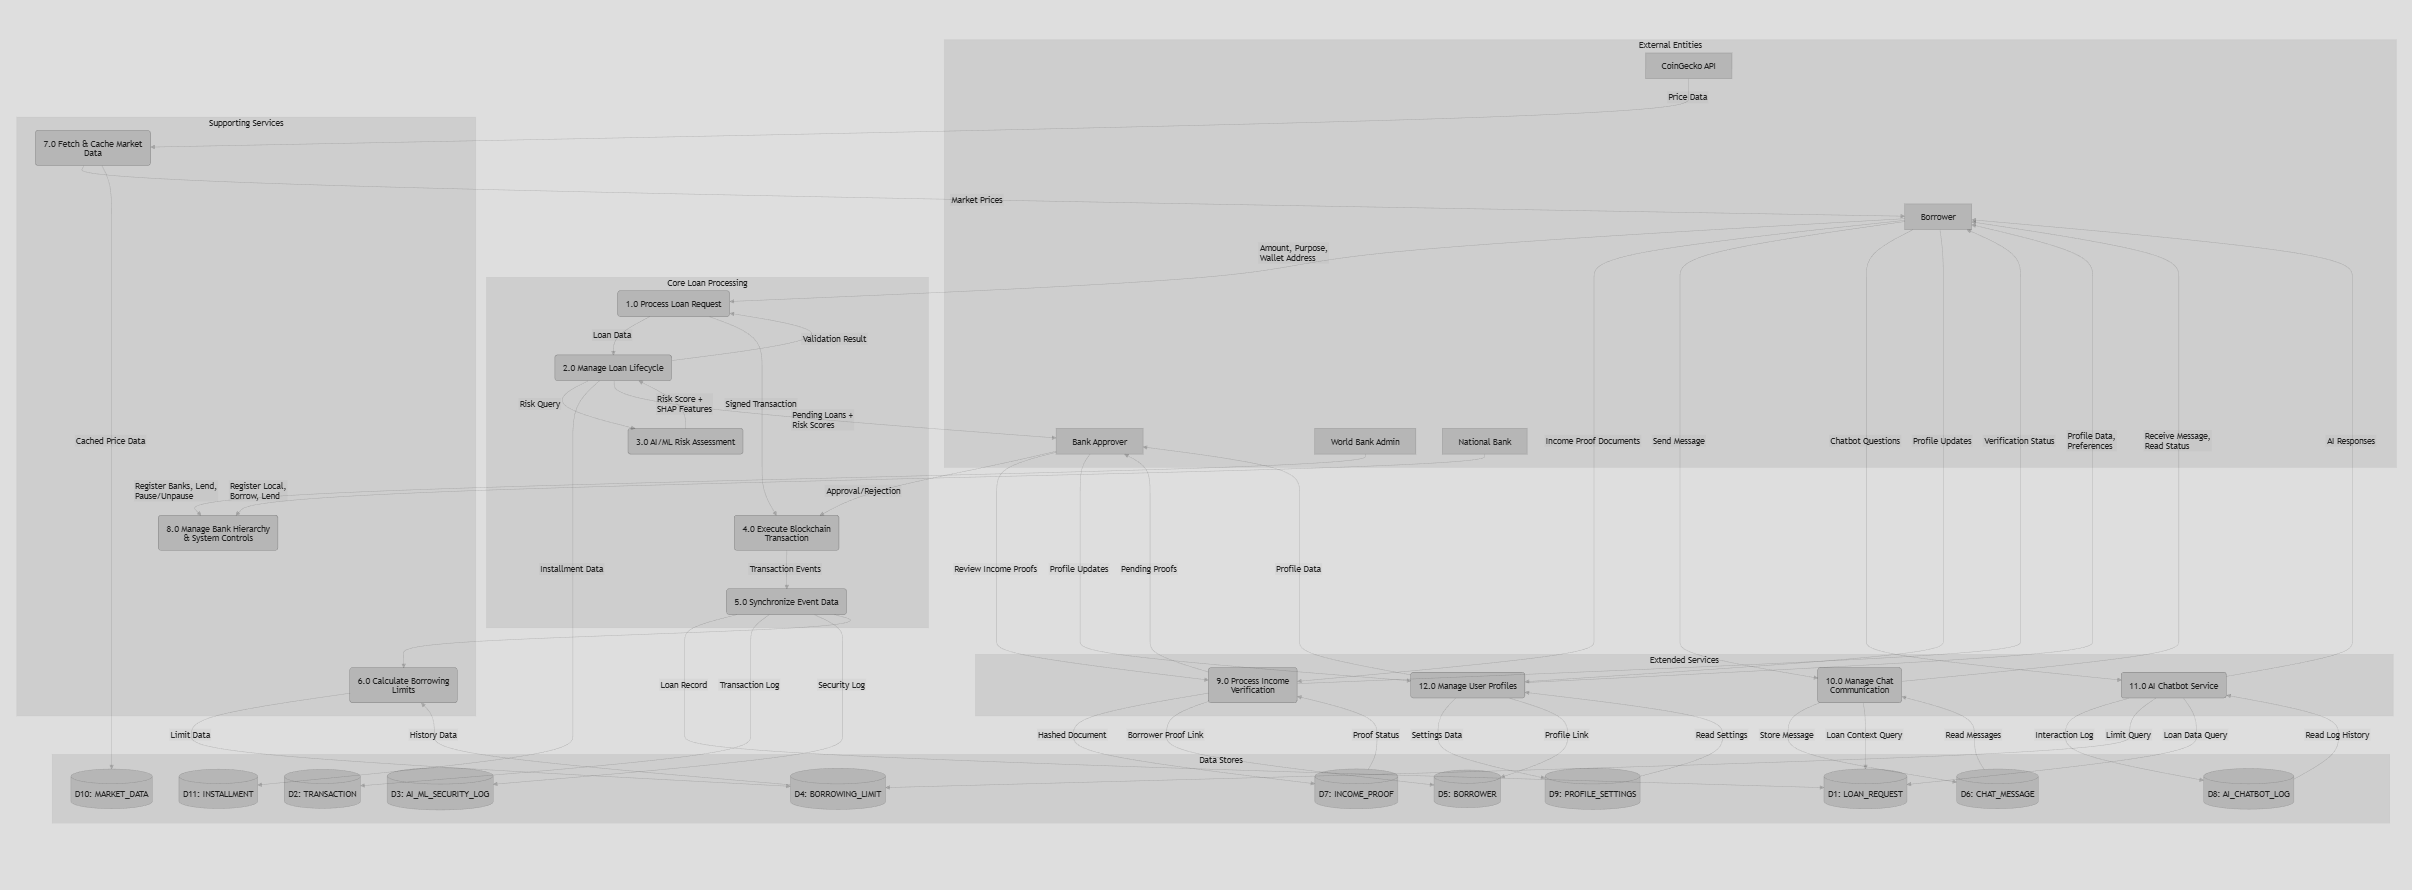
\includegraphics[width=\textwidth,keepaspectratio]{Data flow diagram (level - 1).png}
\caption{Data flow diagram --- Level~1 (Part~1) showing decomposed processes, data stores, and information movement across system components.}
\label{fig:dfd-level1a}
\end{figure}

\begin{figure}[H]
\centering
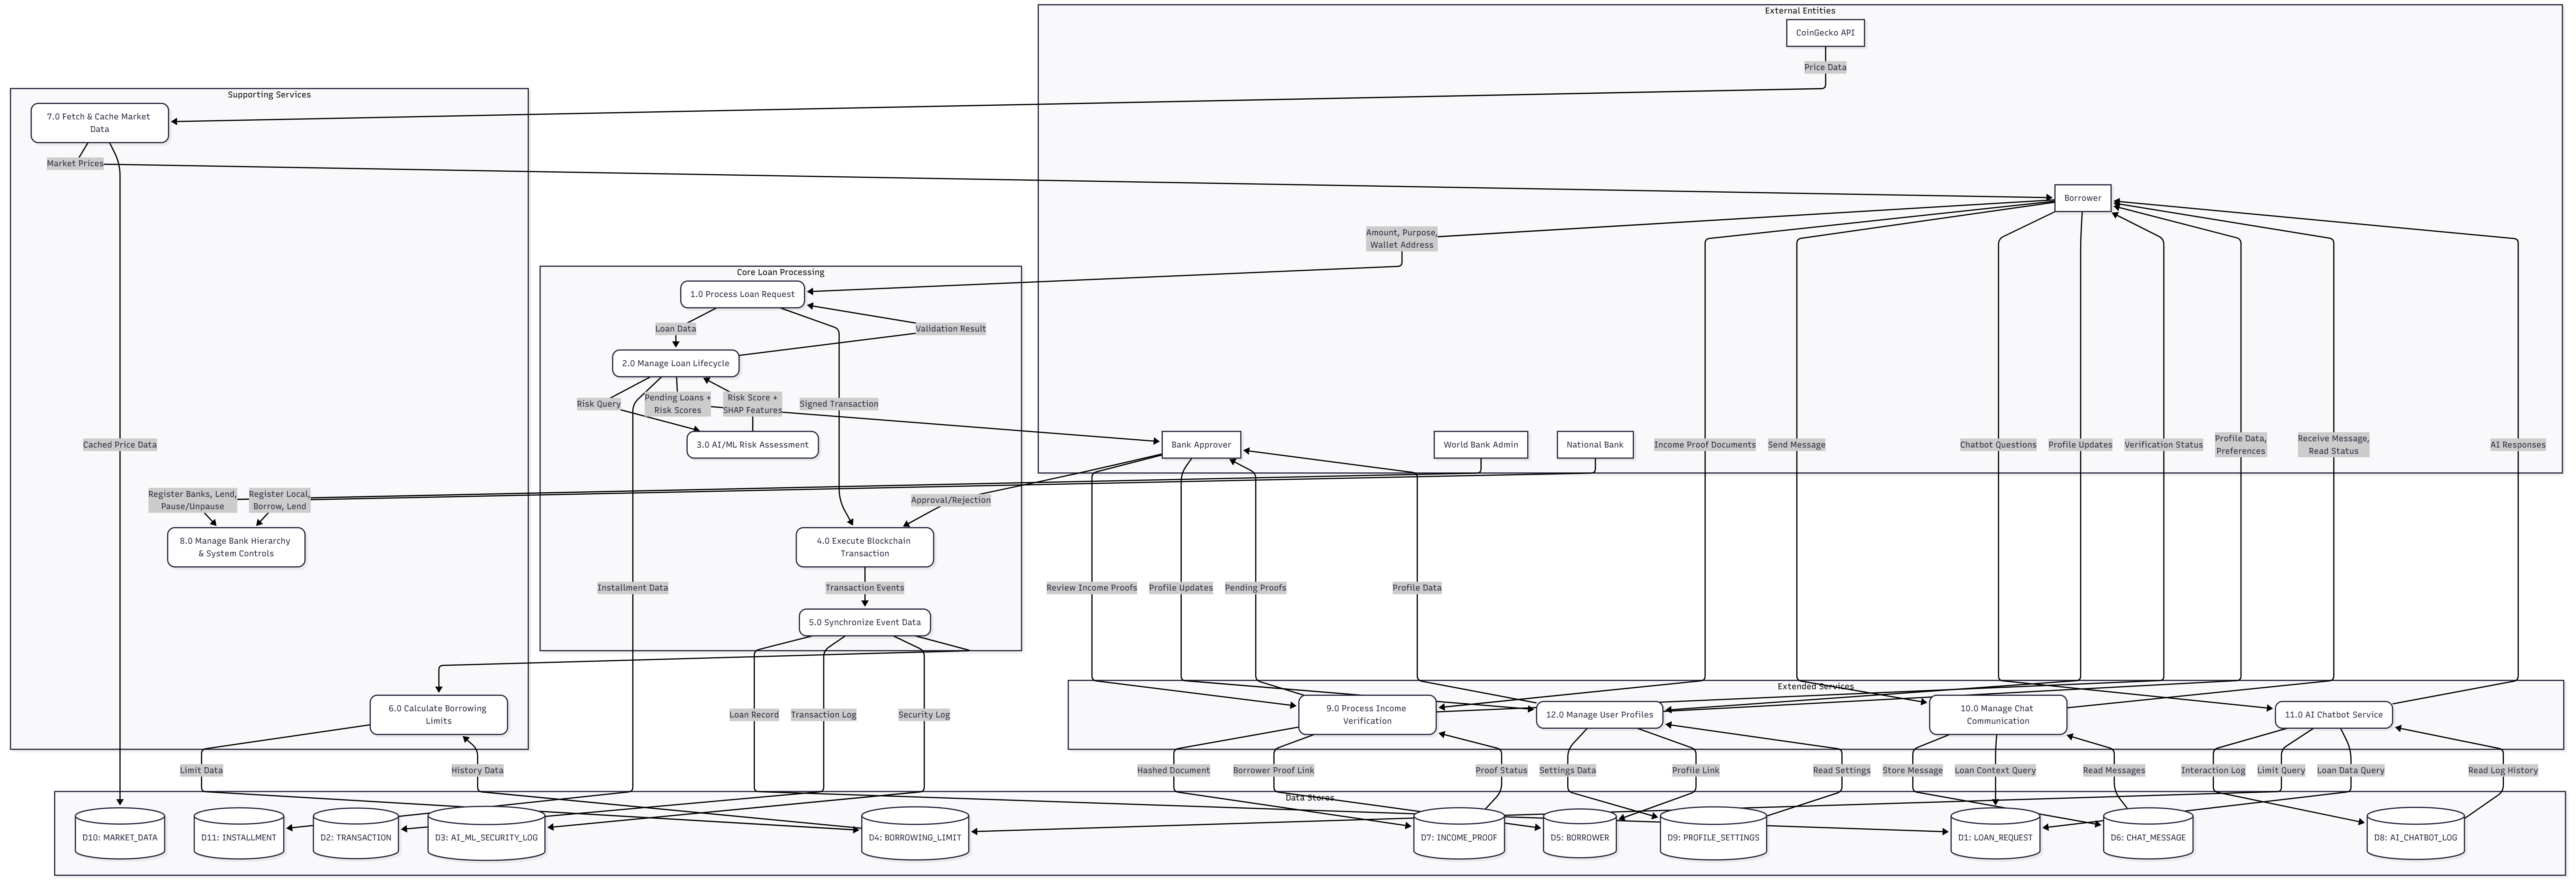
\includegraphics[width=\textwidth,keepaspectratio]{dataflow diagram 2 (level -1).png}
\caption{Data flow diagram --- Level~1 (Part~2) showing additional processes for AI/ML analytics, market data, and profile management.}
\label{fig:dfd-level1b}
\end{figure}

\subsection{Sequence Diagrams}

Figures~\ref{fig:seq-loan}--\ref{fig:seq-borrowlimit} present the sequence diagrams for the platform's key interaction flows.

\begin{figure}[H]
\centering
\includegraphics[width=\textwidth,keepaspectratio]{Sequence Diagram 1 Loan Request, AI Risk Check, and Approval Decision.png}
\caption{Sequence diagram: Loan request, AI risk check, and approval decision across 9 participants.}
\label{fig:seq-loan}
\end{figure}

\begin{figure}[H]
\centering
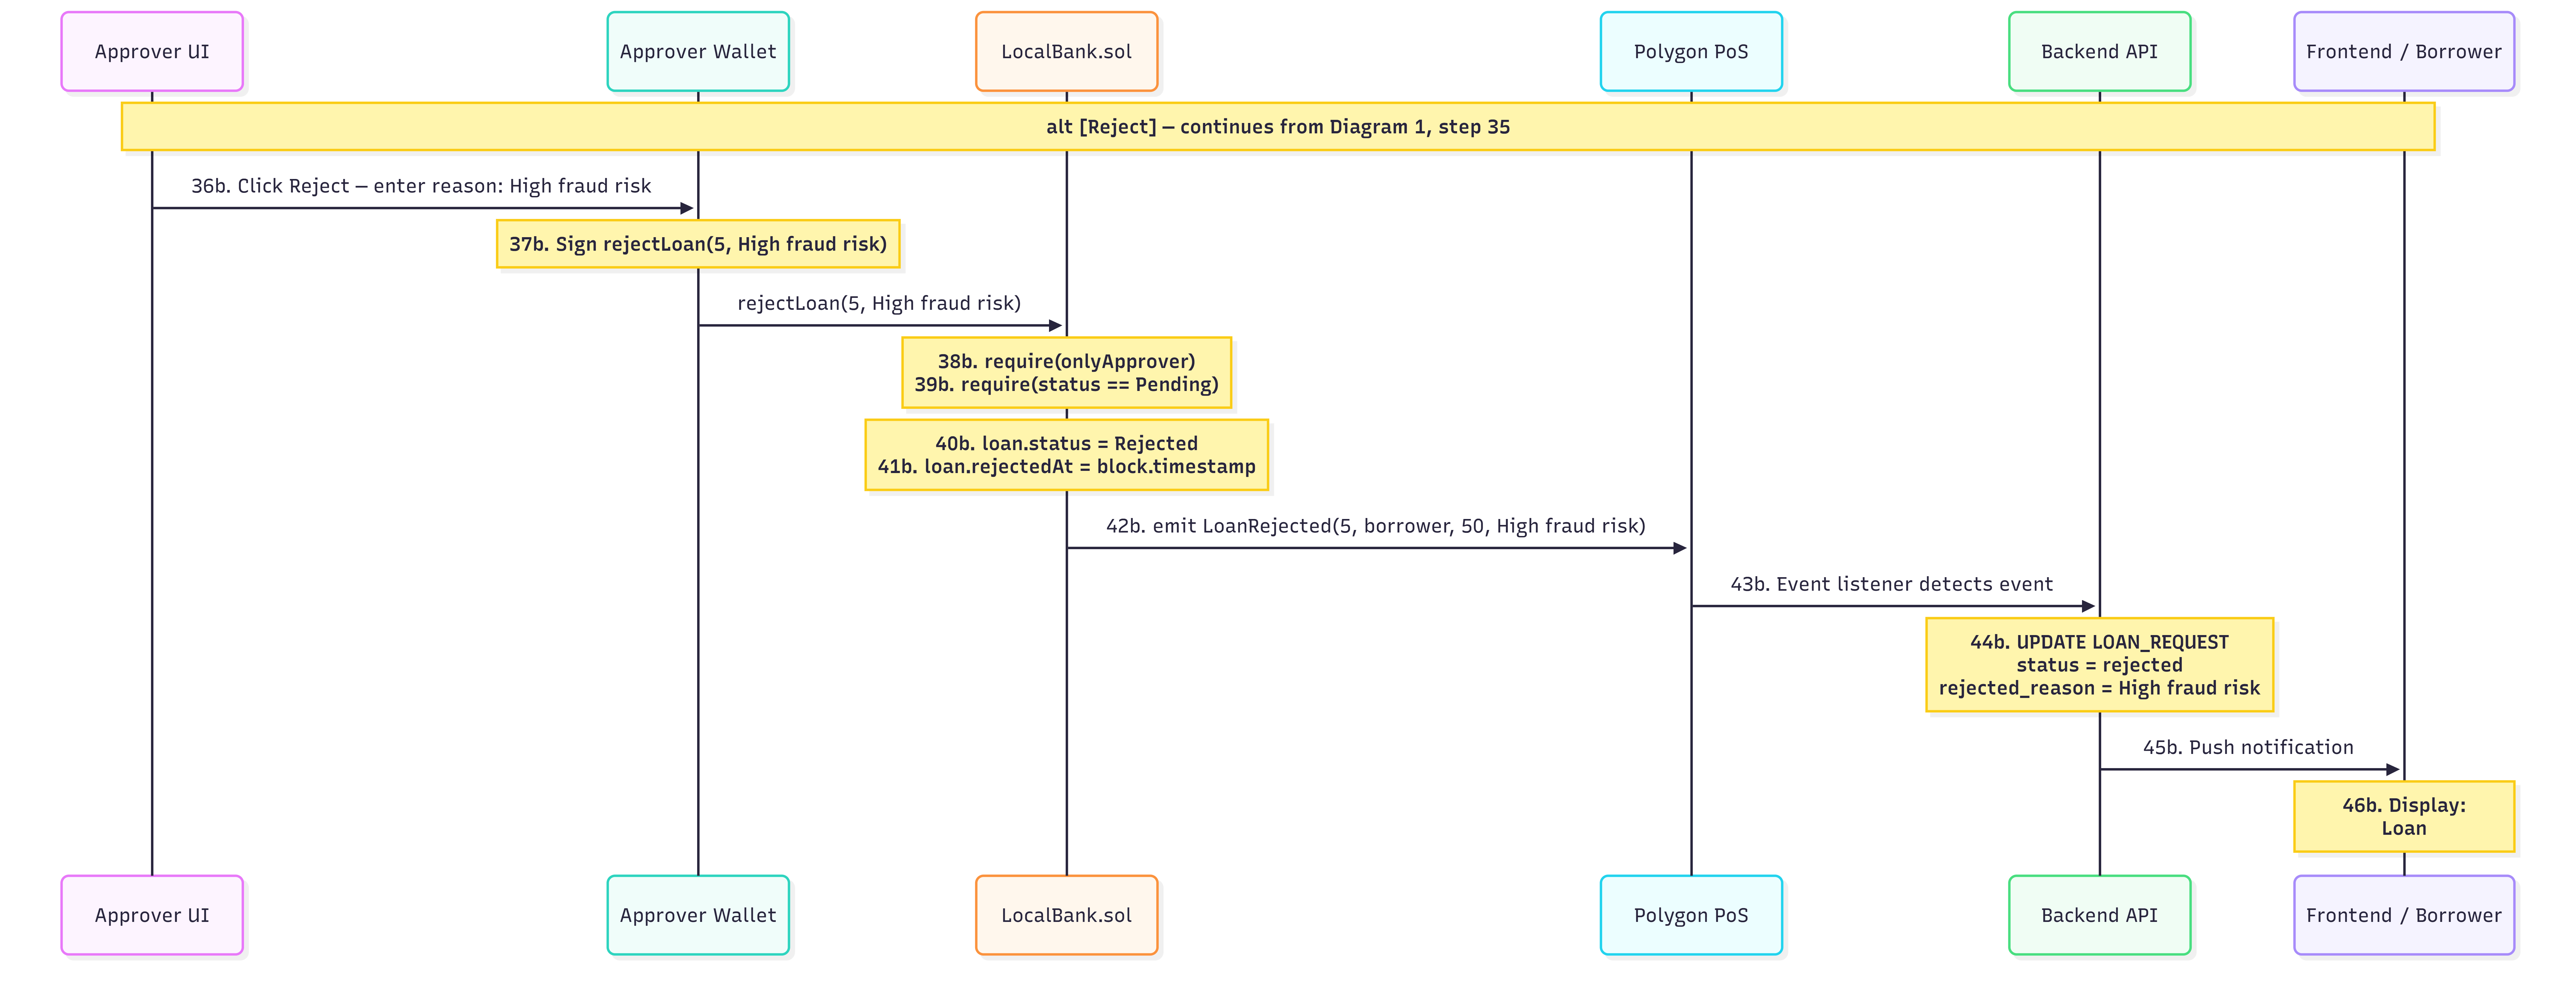
\includegraphics[width=\textwidth,keepaspectratio]{Sequence Diagram 1B Reject Path - alt Reject.png}
\caption{Sequence diagram: Reject path (alternative flow) for loan request denial.}
\label{fig:seq-reject}
\end{figure}

\begin{figure}[H]
\centering
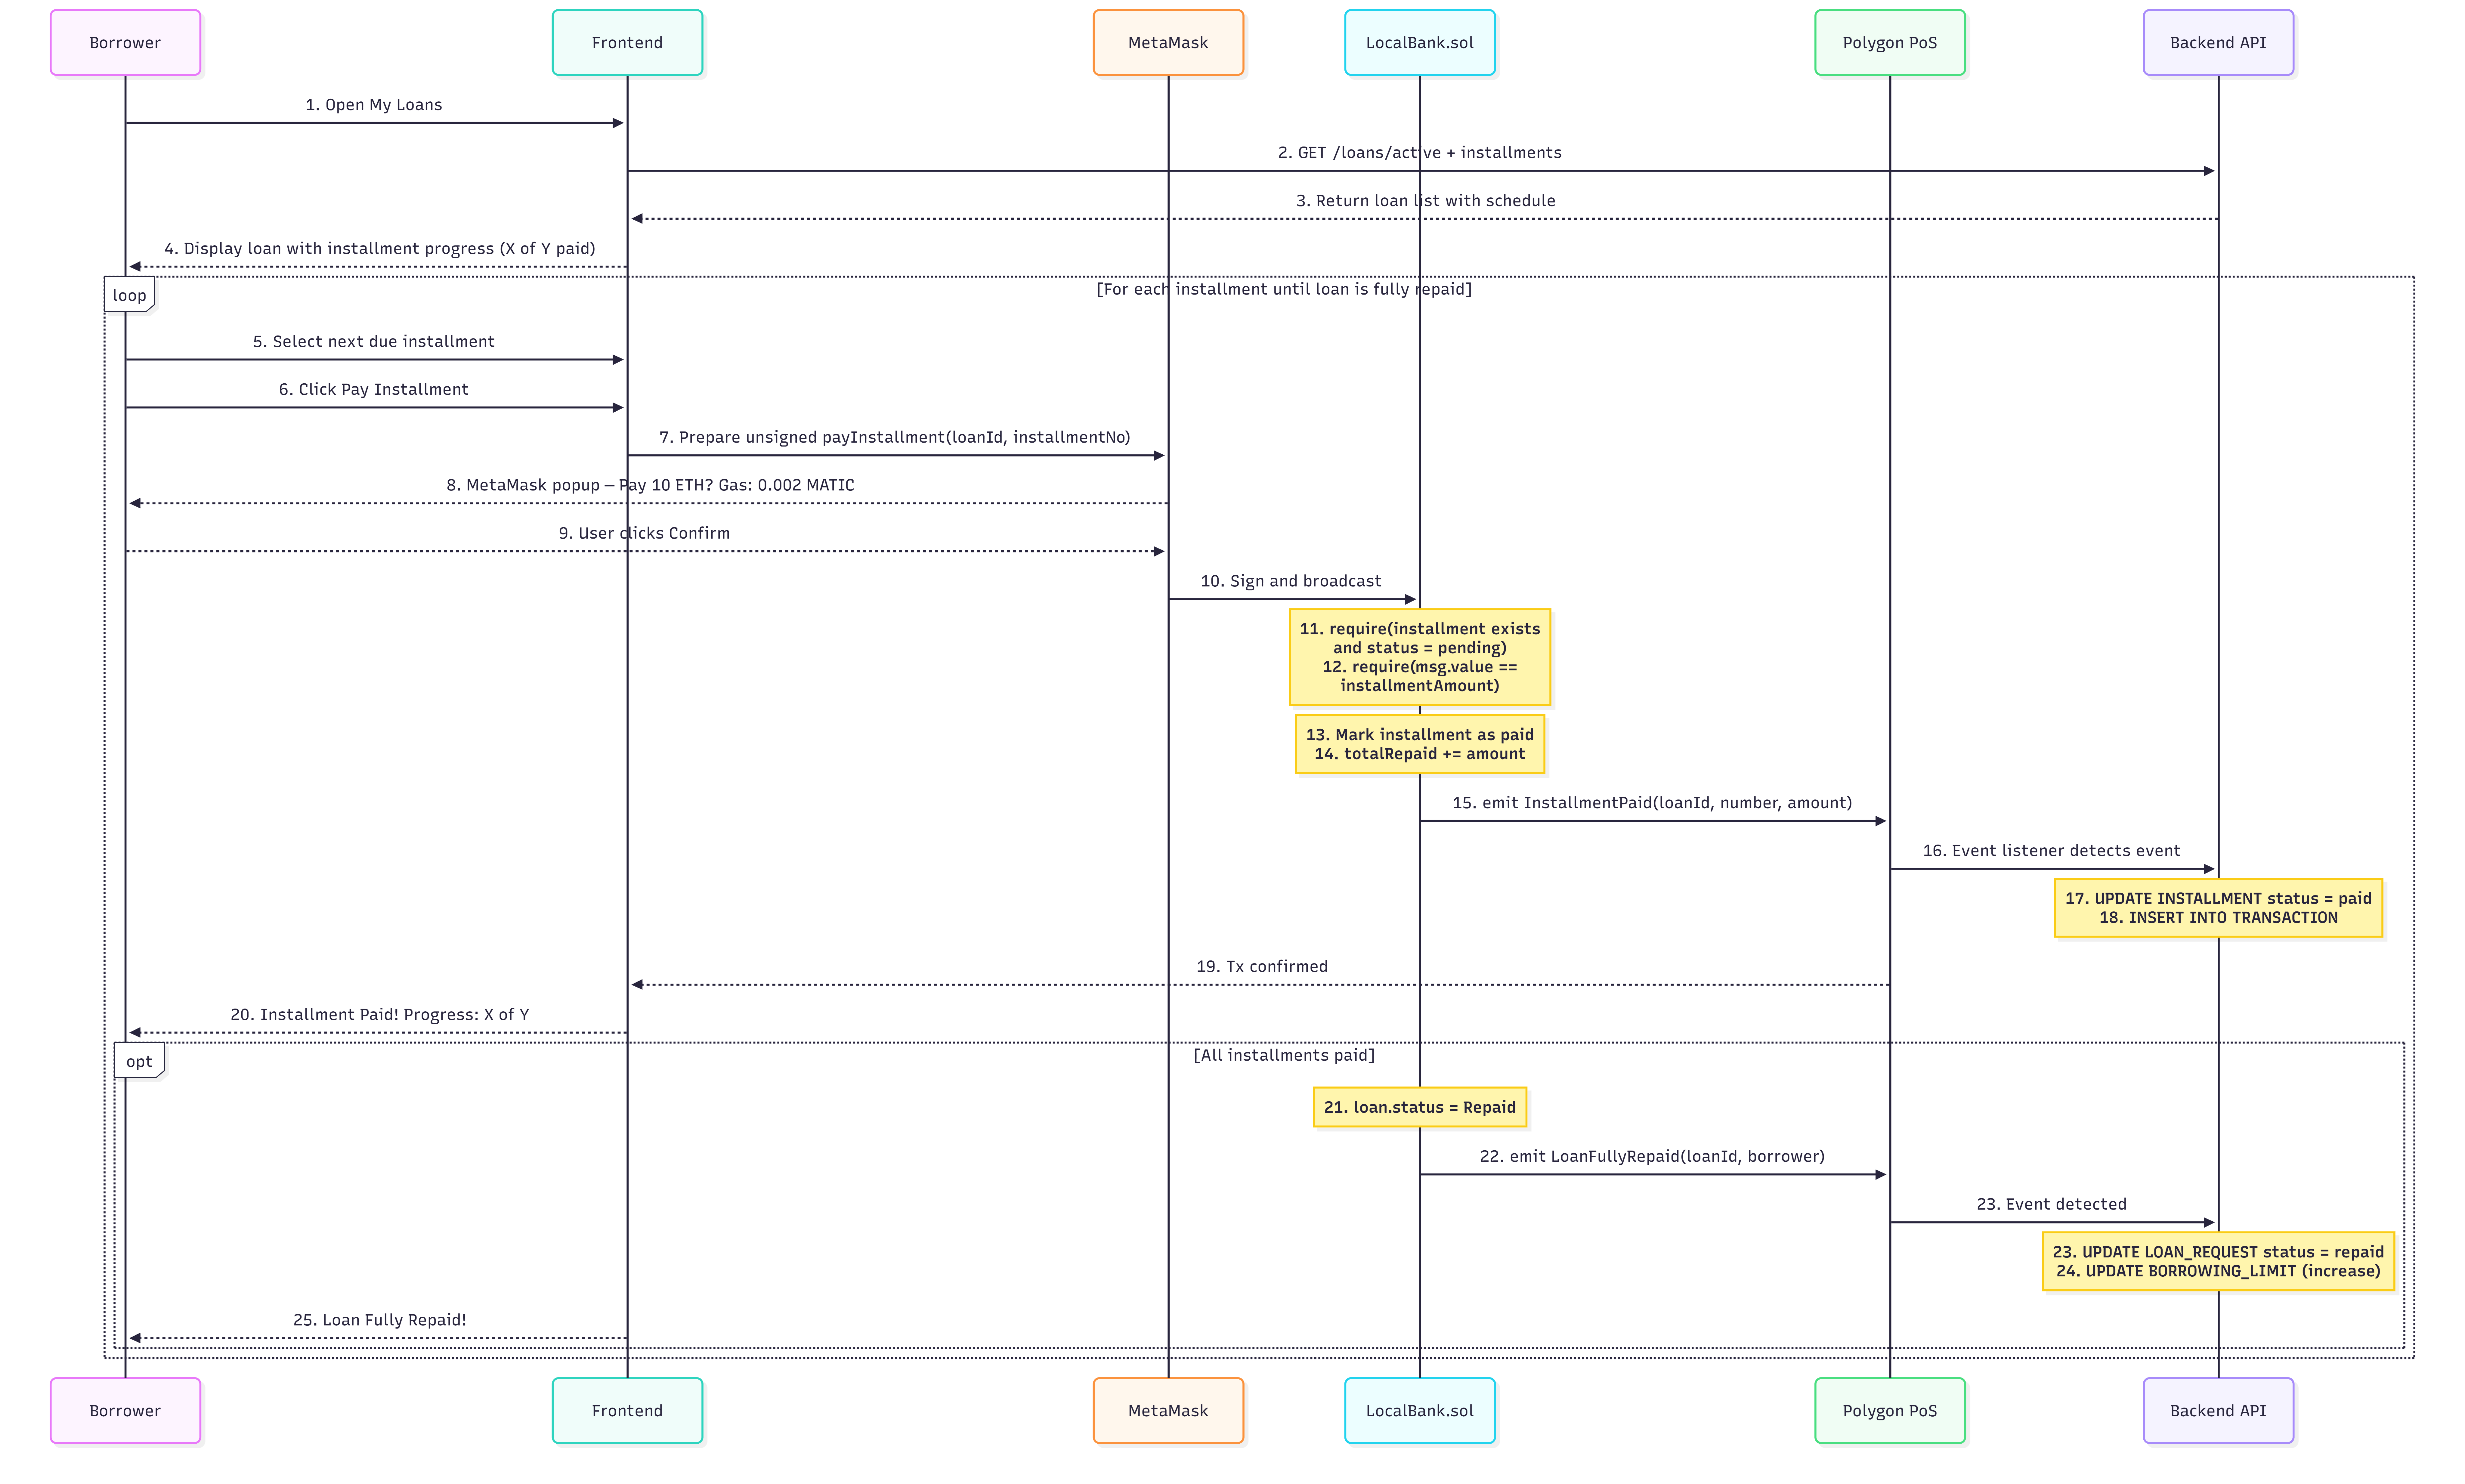
\includegraphics[width=\textwidth,keepaspectratio]{Sequence Diagram 2 Installment Payment Loop.png}
\caption{Sequence diagram: Installment payment loop showing recurring payment processing and balance updates.}
\label{fig:seq-installment}
\end{figure}

\begin{figure}[H]
\centering
\includegraphics[width=\textwidth,keepaspectratio]{Sequence Diagram 3 Income Verification.png}
\caption{Sequence diagram: Income verification process between borrower, frontend, backend API, and database.}
\label{fig:seq-income}
\end{figure}

\begin{figure}[H]
\centering
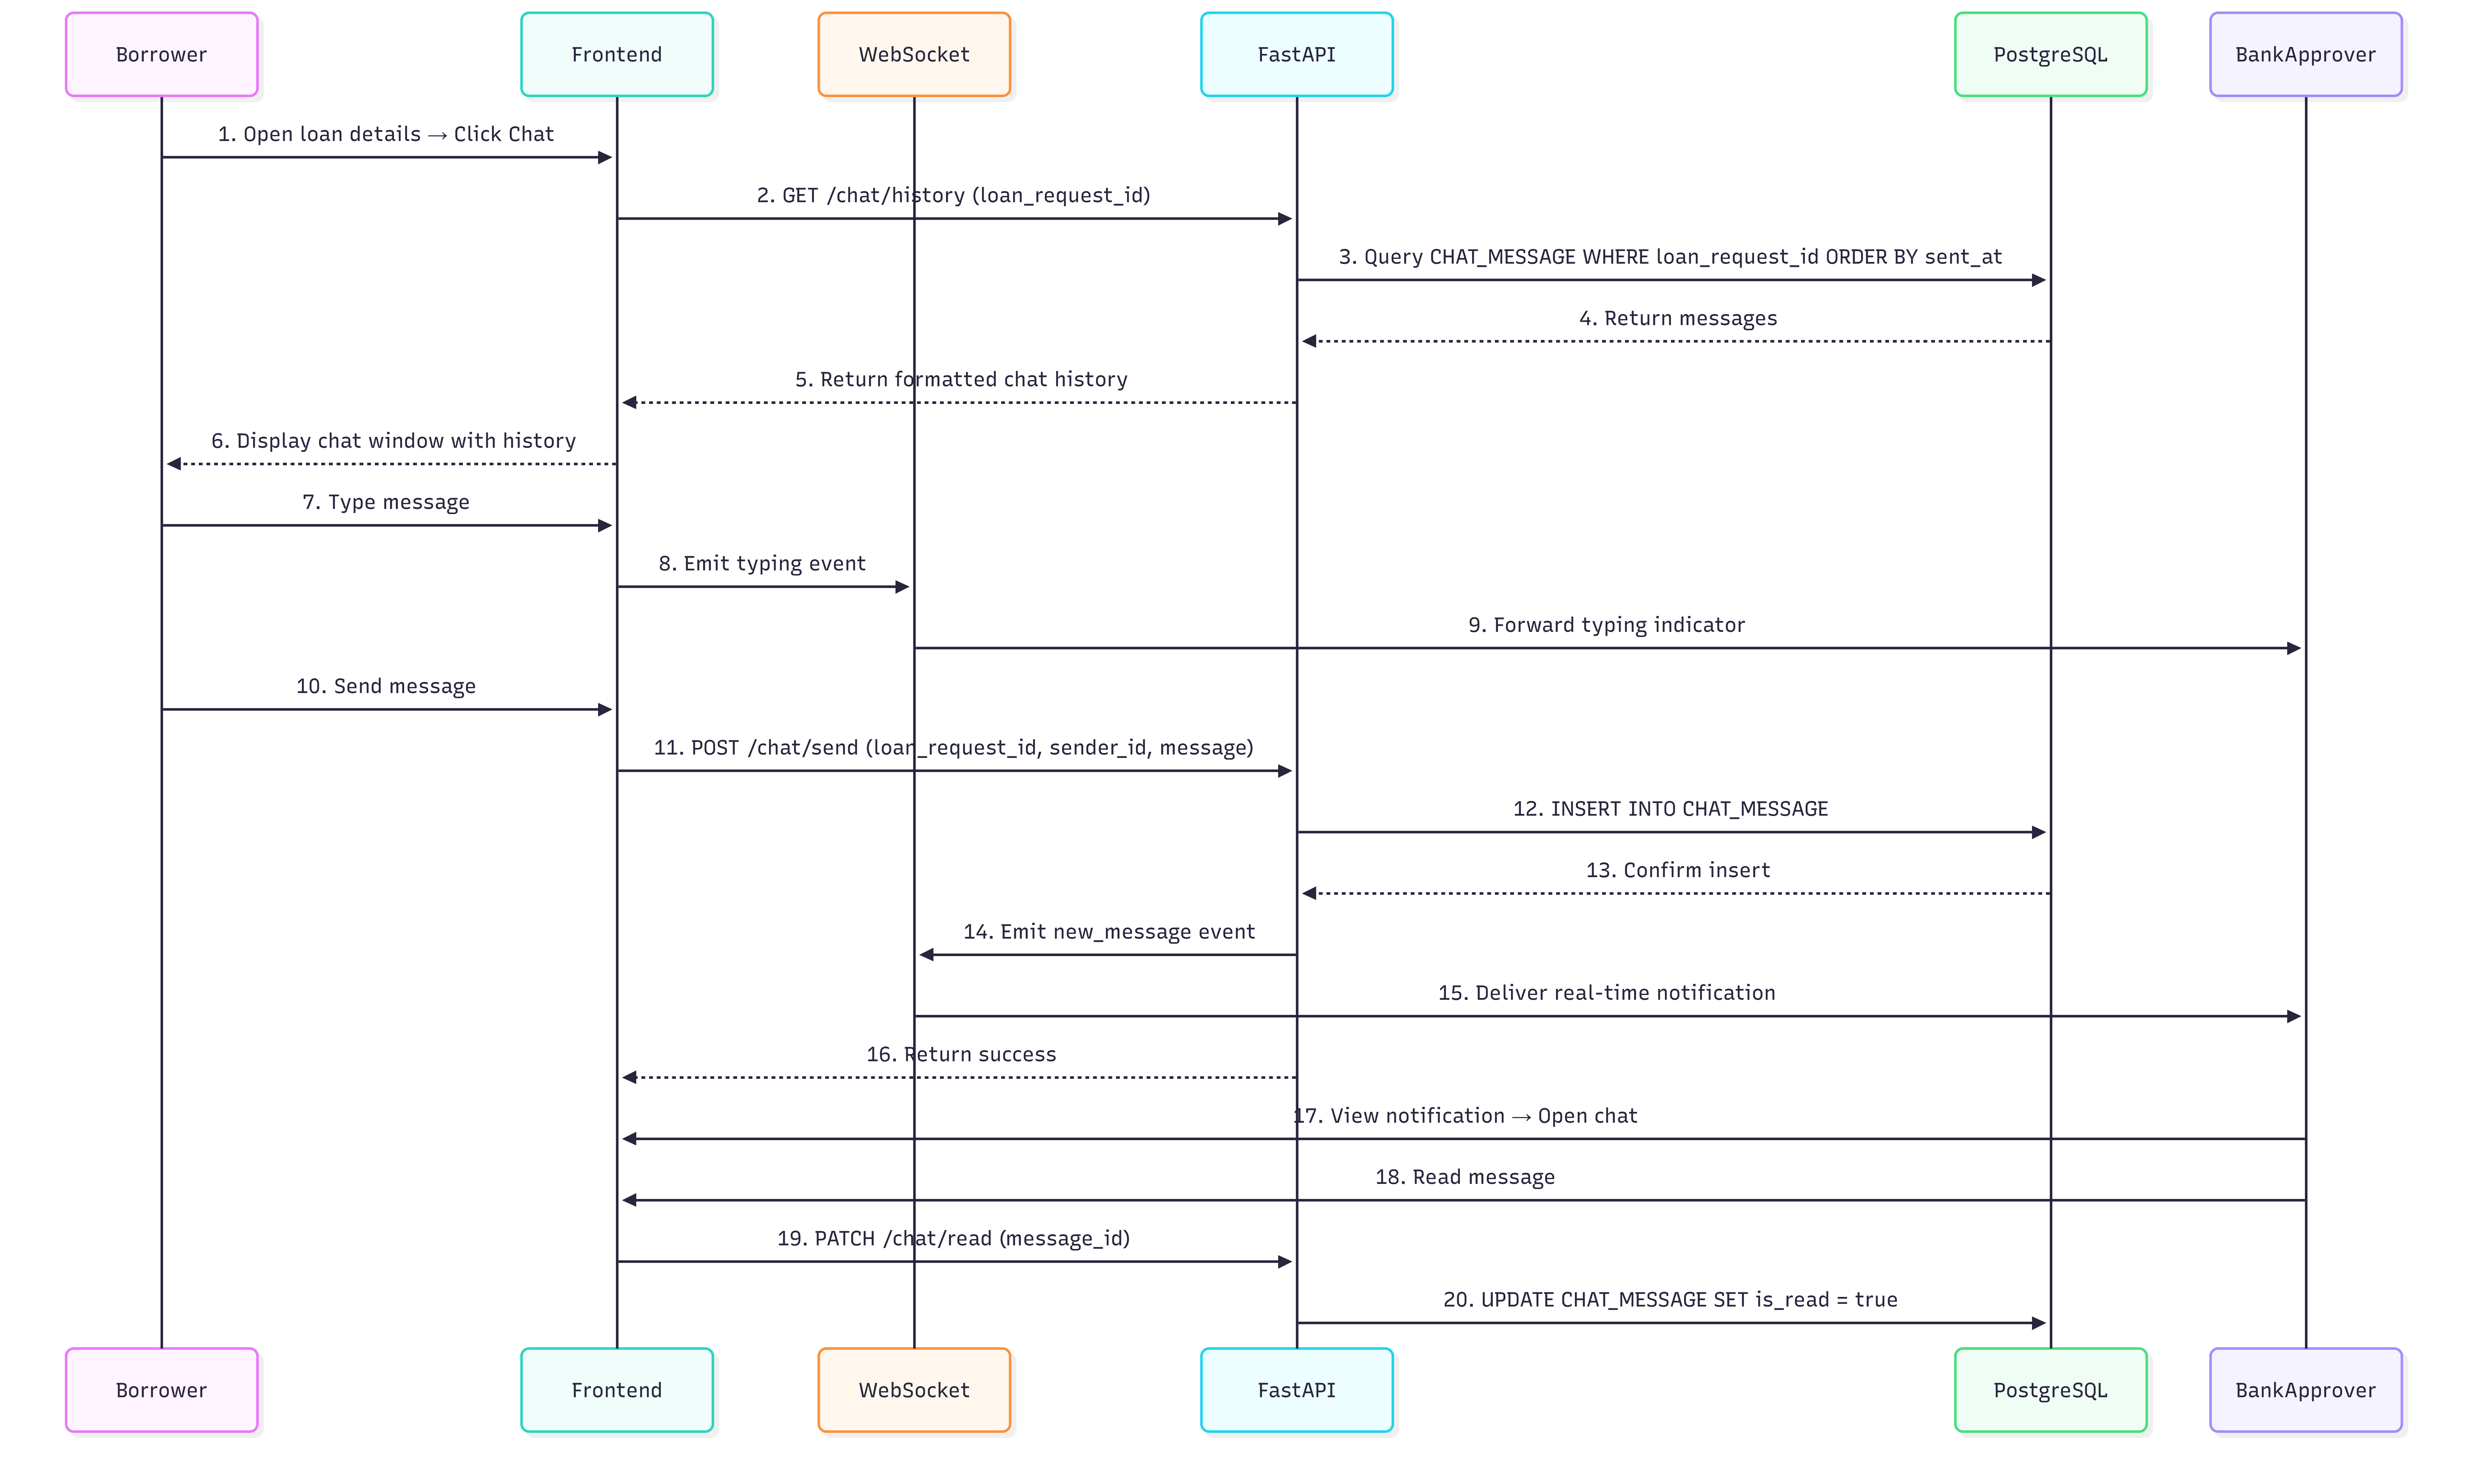
\includegraphics[width=\textwidth,keepaspectratio]{Sequence Diagram 4 Chat System.png}
\caption{Sequence diagram: Chat system message exchange between borrower and bank representative.}
\label{fig:seq-chat}
\end{figure}

\begin{figure}[H]
\centering
\includegraphics[width=\textwidth,keepaspectratio]{Sequence Diagram 5 AI Chatbot Interaction.png}
\caption{Sequence diagram: AI chatbot interaction for automated borrower support queries.}
\label{fig:seq-aichatbot}
\end{figure}

\begin{figure}[H]
\centering
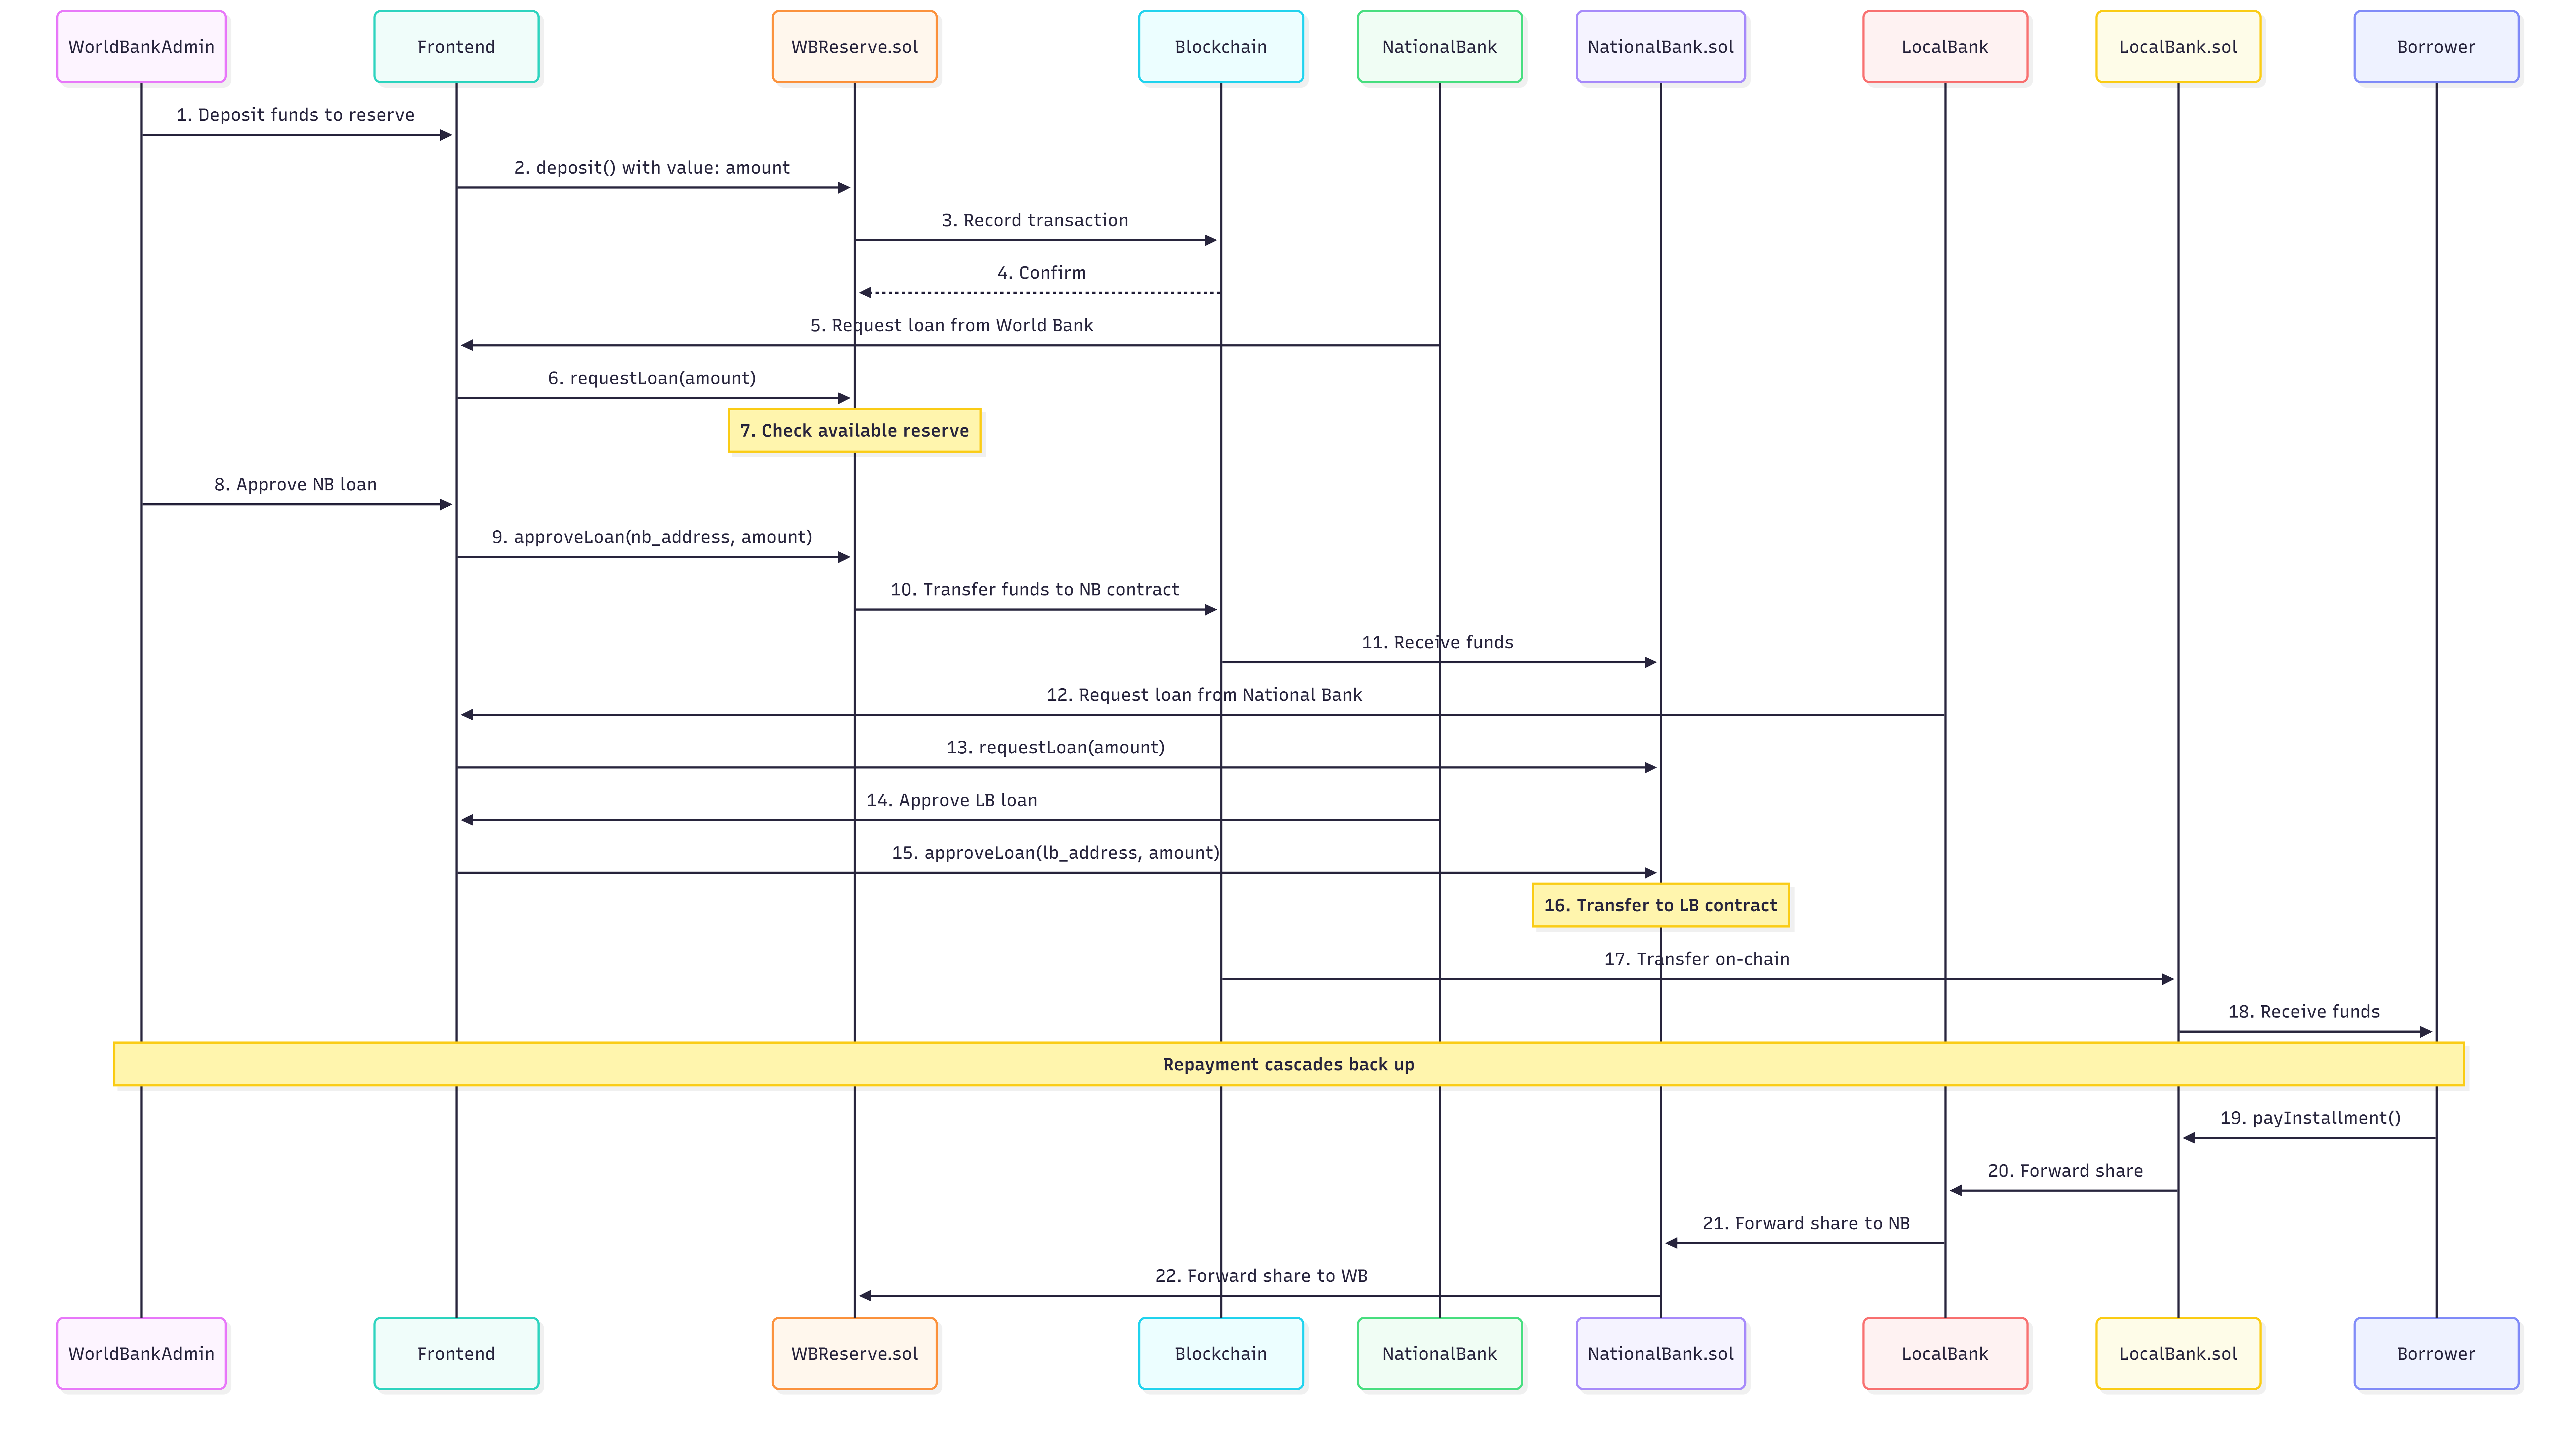
\includegraphics[width=\textwidth,keepaspectratio]{Sequence Diagram 6 Hierarchical Banking.png}
\caption{Sequence diagram: Hierarchical banking flow showing capital distribution from World Bank through National and Local Banks to Borrowers.}
\label{fig:seq-hierarchy}
\end{figure}

\begin{figure}[H]
\centering
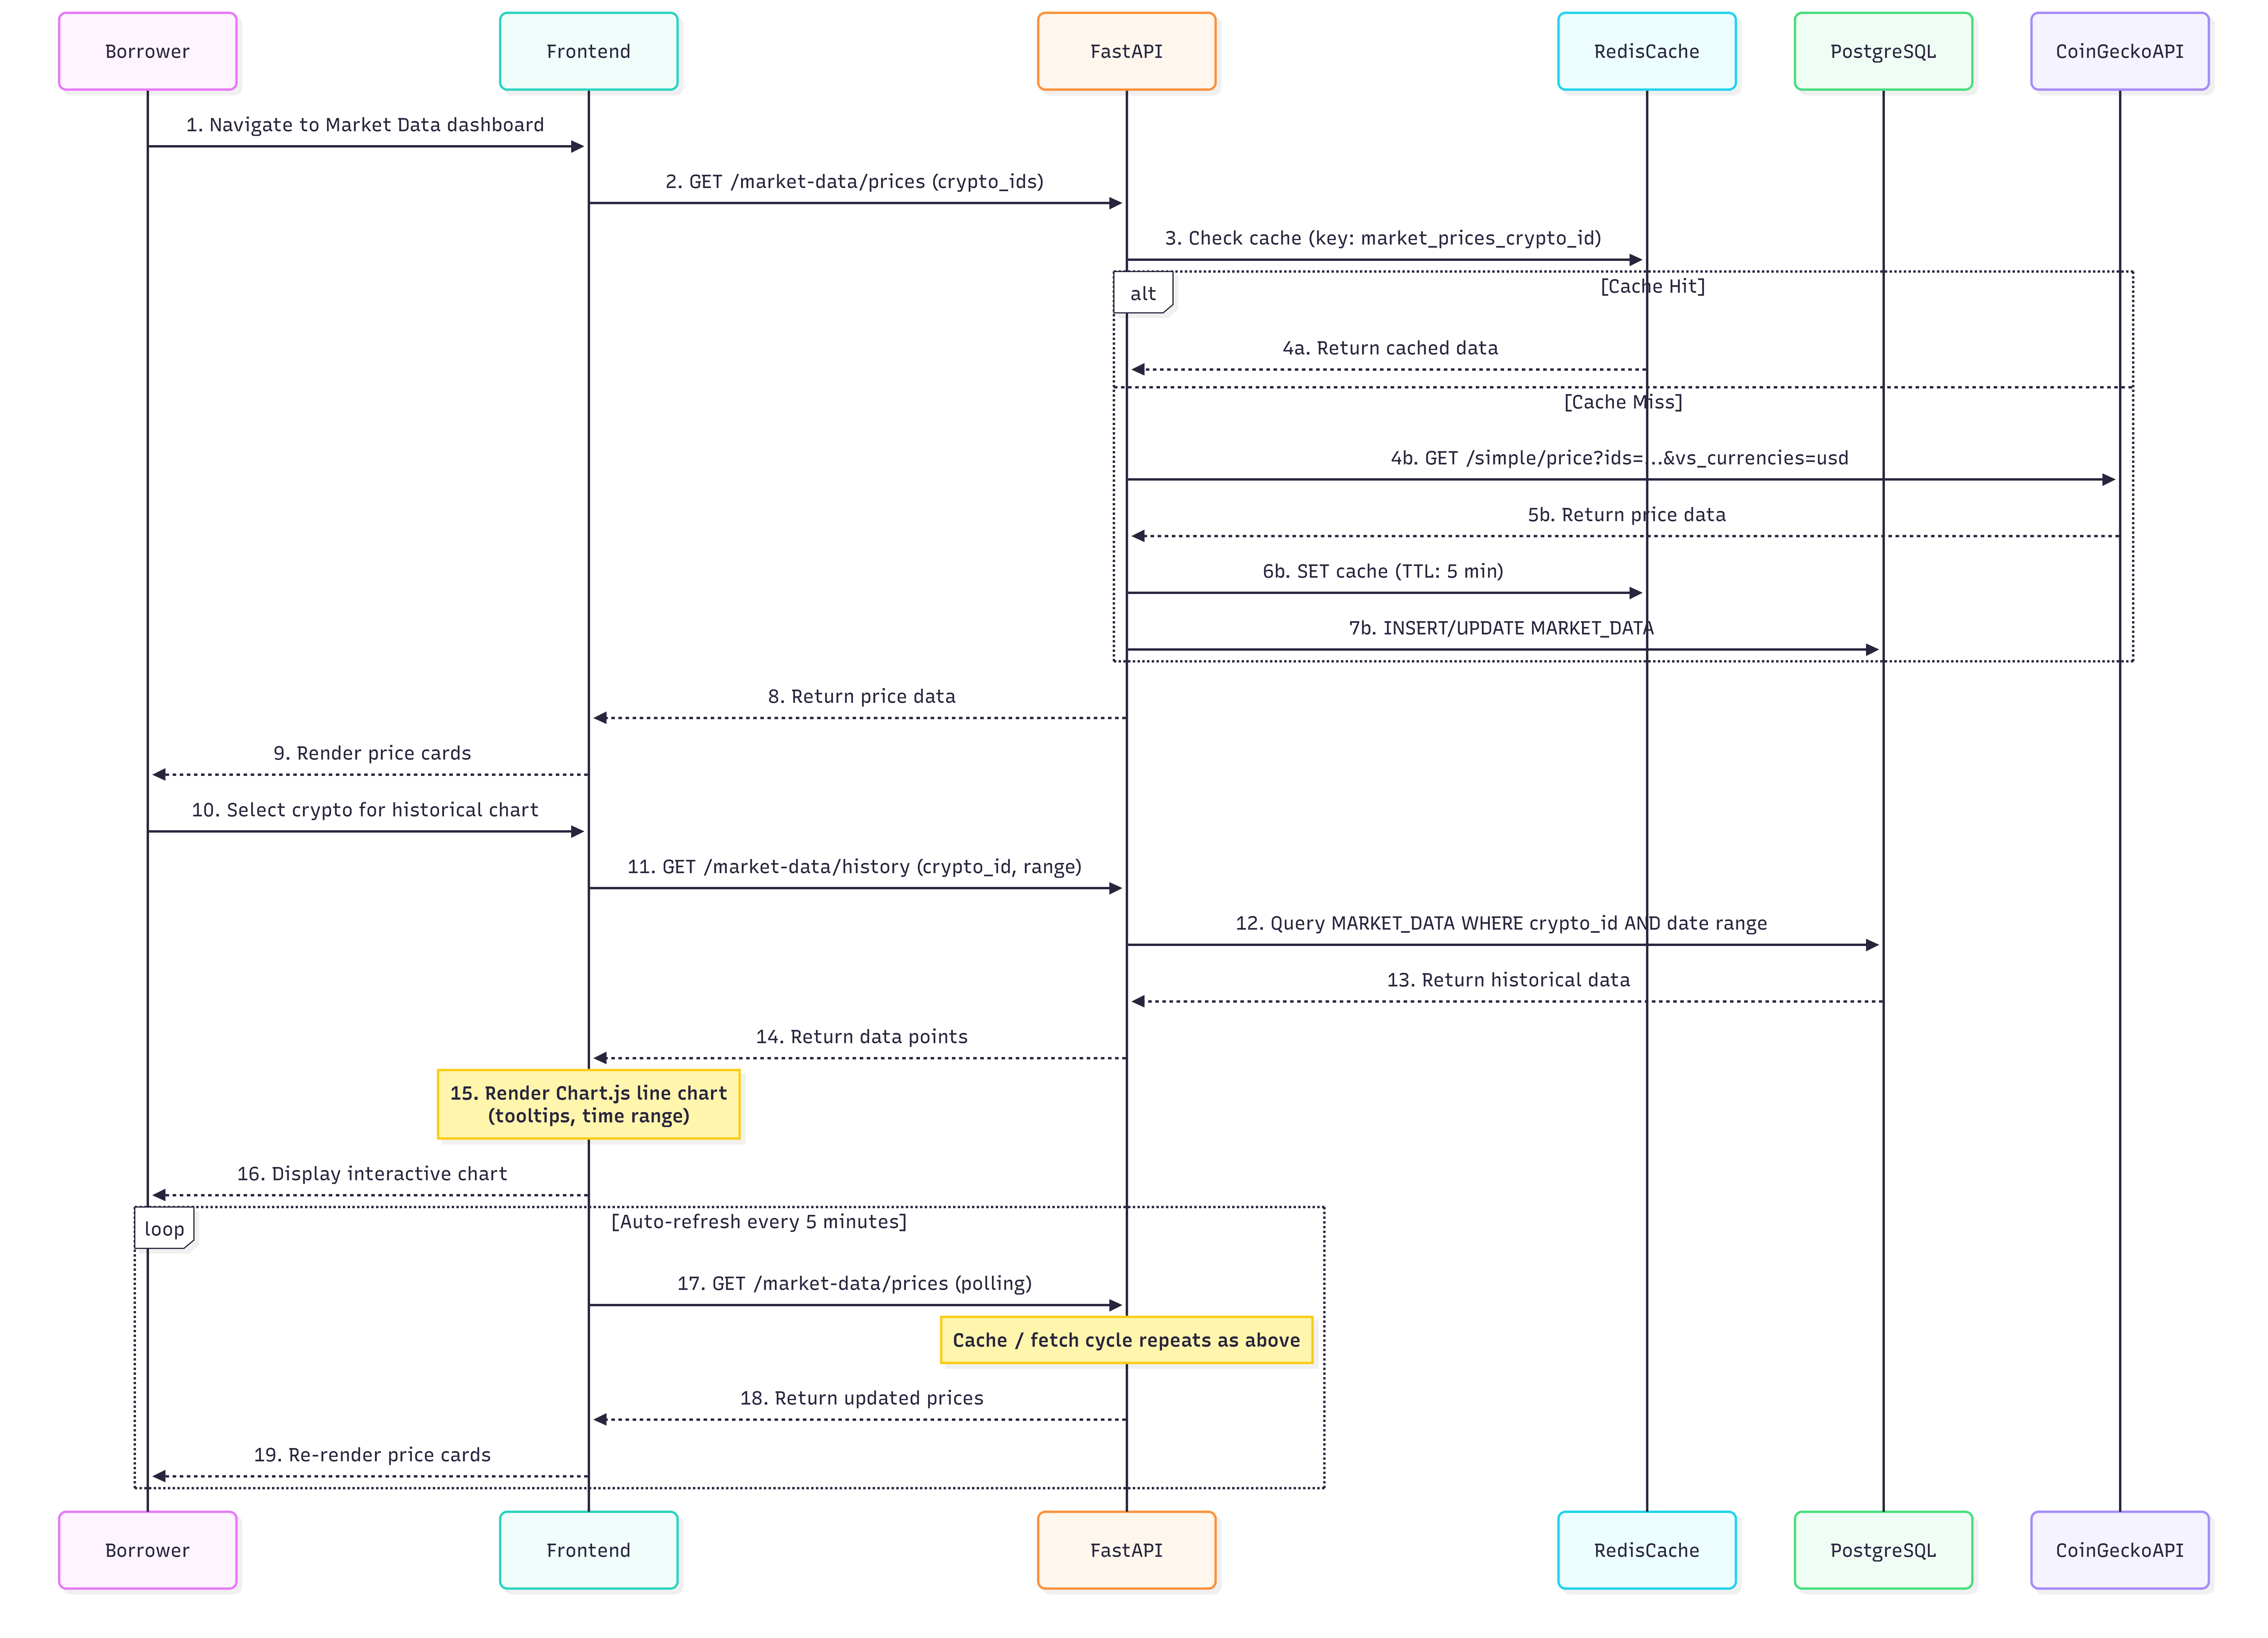
\includegraphics[width=\textwidth,keepaspectratio]{Sequence Diagram 7 Market Data Retrieval.png}
\caption{Sequence diagram: Market data retrieval from external cryptocurrency price APIs.}
\label{fig:seq-marketdata}
\end{figure}

\begin{figure}[H]
\centering
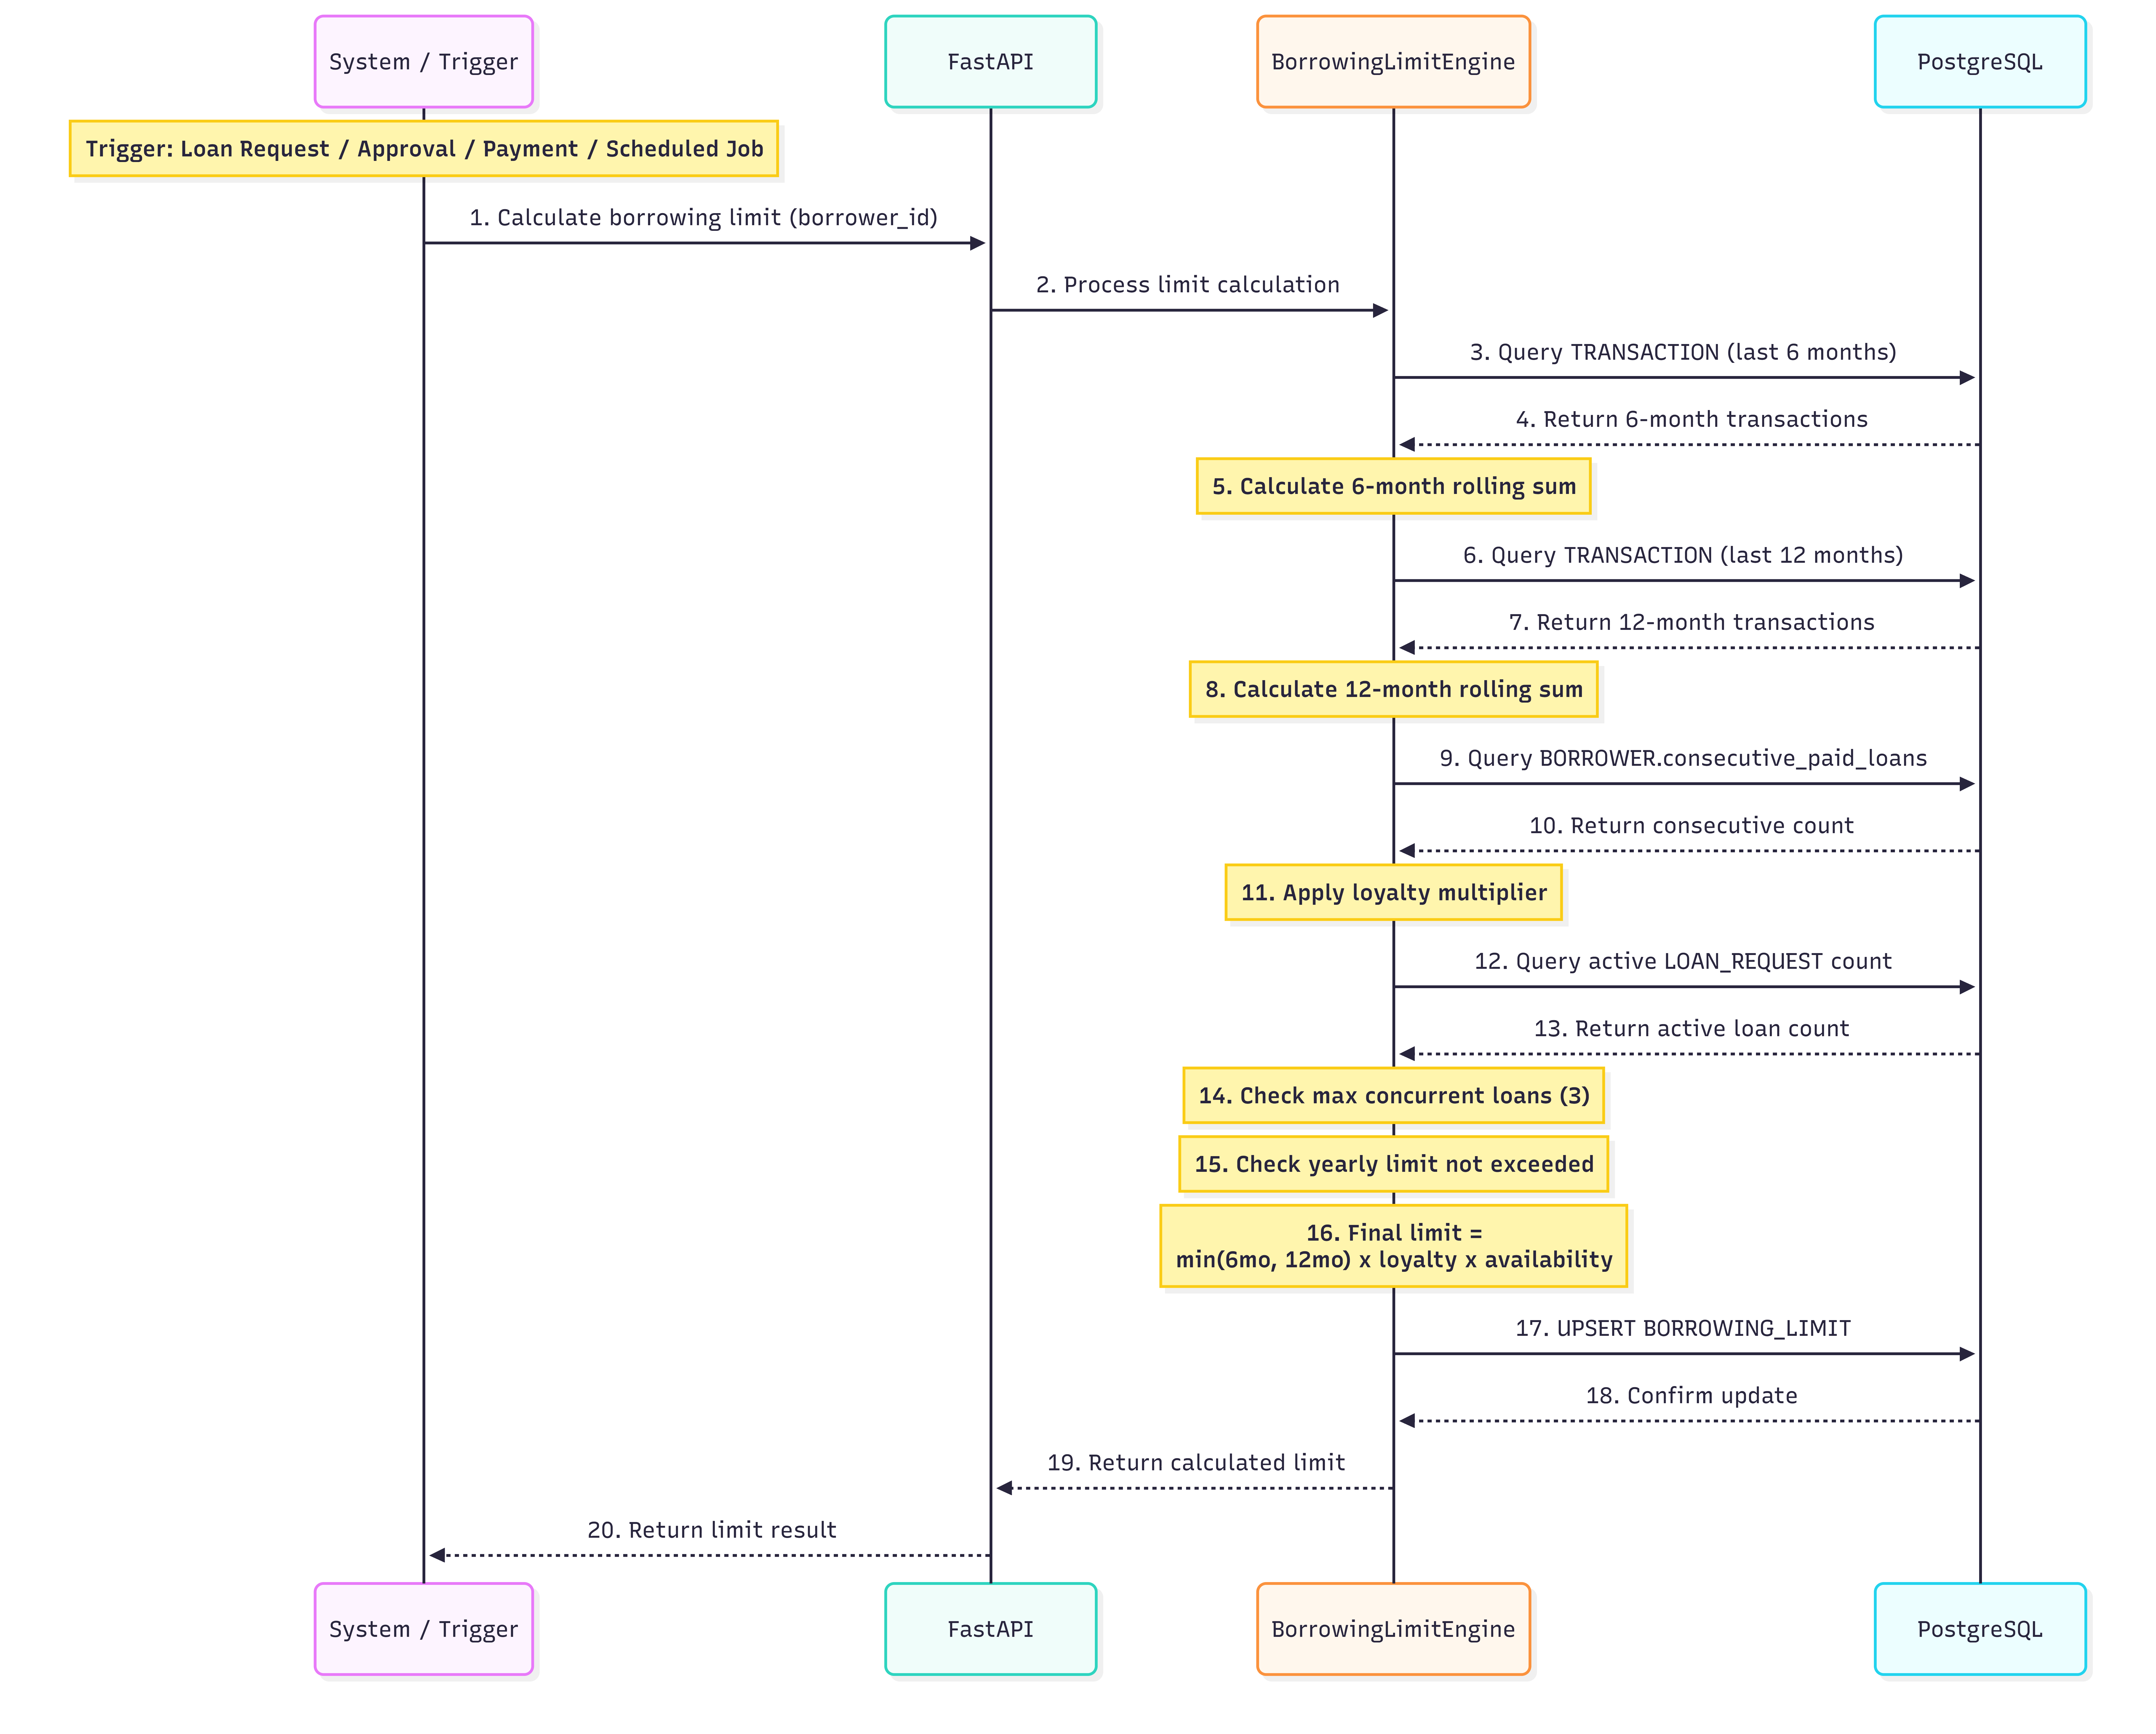
\includegraphics[width=\textwidth,keepaspectratio]{Sequence Diagram 8 Borrowing Limit Calculation.png}
\caption{Sequence diagram: Borrowing limit calculation using rolling 6-month and 1-year transaction windows.}
\label{fig:seq-borrowlimit}
\end{figure}

\subsection{Four-Tier Capital Flow}

Figure~\ref{fig:four-tier} illustrates the hierarchical capital flow and cascading repayment structure.

\begin{figure}[H]
\centering
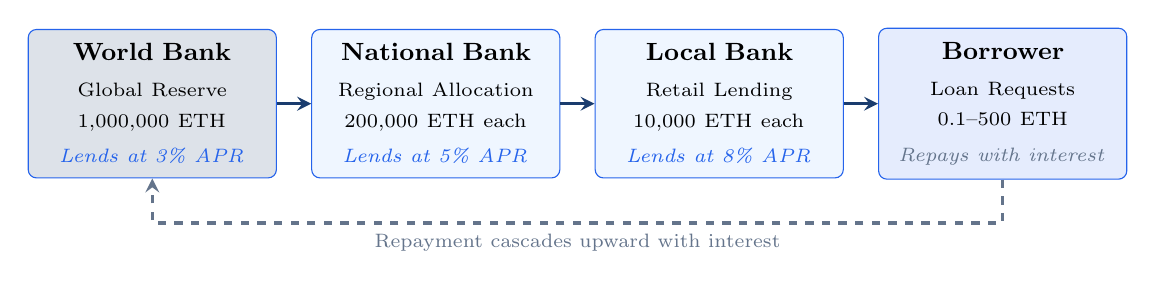
\begin{tikzpicture}[
    tier/.style={
        draw=AccentBlue,
        fill=LightBlue,
        rounded corners=3pt,
        minimum width=3cm,
        minimum height=1.8cm,
        text width=2.8cm,
        align=center,
        font=\small,
        inner sep=5pt,
    },
    tierarrow/.style={
        ->,
        >=stealth,
        line width=1.2pt,
        color=PrimaryBlue,
    },
]
\node[tier,fill=PrimaryBlue!15] (wb) at (0,0) {%
    \textbf{World Bank}\\[2pt]
    {\scriptsize Global Reserve}\\
    {\scriptsize 1,000,000 ETH}\\[2pt]
    {\scriptsize\color{AccentBlue}\textit{Lends at 3\% APR}}};

\node[tier] (nb) at (3.6,0) {%
    \textbf{National Bank}\\[2pt]
    {\scriptsize Regional Allocation}\\
    {\scriptsize 200,000 ETH each}\\[2pt]
    {\scriptsize\color{AccentBlue}\textit{Lends at 5\% APR}}};

\node[tier] (lb) at (7.2,0) {%
    \textbf{Local Bank}\\[2pt]
    {\scriptsize Retail Lending}\\
    {\scriptsize 10,000 ETH each}\\[2pt]
    {\scriptsize\color{AccentBlue}\textit{Lends at 8\% APR}}};

\node[tier,fill=AccentBlue!12] (br) at (10.8,0) {%
    \textbf{Borrower}\\[2pt]
    {\scriptsize Loan Requests}\\
    {\scriptsize 0.1--500 ETH}\\[2pt]
    {\scriptsize\color{GrayText}\textit{Repays with interest}}};

\draw[tierarrow] (wb) -- (nb);
\draw[tierarrow] (nb) -- (lb);
\draw[tierarrow] (lb) -- (br);

\draw[tierarrow,dashed,color=GrayText] (br.south) -- ++(0,-0.55) -| node[below,pos=0.25,font=\scriptsize,color=GrayText] {Repayment cascades upward with interest} (wb.south);
\end{tikzpicture}
\caption{Four-tier hierarchical capital flow with cascading repayment.}
\label{fig:four-tier}
\end{figure}


\section{Auxiliary Dual-Currency Facility}

The Crypto World Bank's cryptocurrency exchange capability is designed as an \textbf{auxiliary facility} integrated into existing banking infrastructure worldwide. Rather than operating as a standalone exchange, the platform extends the services of participating banks by enabling a dual-currency feature---allowing eligible bank customers to transact in both fiat and cryptocurrency within their existing banking relationship.

\begin{itemize}[noitemsep]
\item \textbf{Integration model:} The dual-currency facility is offered by all participating banks as an add-on service to their existing product portfolio. No new banking license or standalone entity is required.
\item \textbf{Eligibility determination:} Eligibility for dual-currency services is determined by the bank officers who manage lending operations, based on existing KYC/AML compliance, account standing, and lending relationship history.
\item \textbf{No defaulting of conditions:} The project does not override, modify, or default any existing banking conditions, regulatory requirements, or contractual obligations.
\item \textbf{Scope:} The facility enables fiat-to-crypto and crypto-to-fiat conversions, cryptocurrency-denominated lending and repayment, and transparent on-chain transaction records---all within the governance structure of the participating bank.
\end{itemize}


\section{Governance Framework}

\subsection{Network Membership Governance}

\begin{moderntable}
\caption{Network membership governance.}
\begin{tabular}{@{} >{\raggedright}p{3.5cm} >{\raggedright\arraybackslash}p{8.5cm} @{}}
\toprule
\tableheadfont Governance Aspect & \tableheadfont Implementation \\
\midrule
\rowcolor{RowShade}
Member on-boarding & World Bank owner registers National Banks; National Banks register Local Banks; Local Banks designate approvers --- all enforced on-chain \\
Member off-boarding & Deactivation flags in smart contracts; cascading access revocation \\
\rowcolor{RowShade}
Regulatory oversight & Audit log emission via smart contract events; planned read-only regulator dashboard \\
Permission structure & Hierarchical: Owner $\to$ National Bank $\to$ Local Bank $\to$ Approver $\to$ Borrower; enforced by on-chain role-check modifiers \\
\rowcolor{RowShade}
Network operations & Pause/unpause mechanism for emergency response; emergency withdrawal for critical situations \\
\bottomrule
\end{tabular}
\end{moderntable}

\subsection{Business Network Governance}

\begin{moderntable}
\caption{Business network governance.}
\begin{tabular}{@{} >{\raggedright}p{3.5cm} >{\raggedright\arraybackslash}p{8.5cm} @{}}
\toprule
\tableheadfont Governance Aspect & \tableheadfont Implementation \\
\midrule
\rowcolor{RowShade}
Business charter & Defined in project documentation; operational parameters codified in smart contract constants \\
Common services & Reserve management, loan lifecycle orchestration, event-driven notification system \\
\rowcolor{RowShade}
Business SLA & Testnet phase: best-effort availability. Production phase: 99.5\% target uptime with multi-region deployment \\
Regulatory compliance & Architecture designed for audit trail generation; data partitioning supports GDPR-style data subject requests \\
\bottomrule
\end{tabular}
\end{moderntable}

\subsection{Technology Infrastructure Governance}

\begin{moderntable}
\caption{Technology infrastructure governance.}
\begin{tabular}{@{} >{\raggedright}p{3.5cm} >{\raggedright\arraybackslash}p{8.5cm} @{}}
\toprule
\tableheadfont Governance Aspect & \tableheadfont Implementation \\
\midrule
\rowcolor{RowShade}
Distributed IT structure & Client-side frontend (decentralized delivery); blockchain layer (fully decentralized); backend API (centralized, horizontally scalable) \\
Technology assessment & Continuous evaluation of EVM alternatives (L2 rollups, sidechains) for cost and performance optimization \\
\rowcolor{RowShade}
On-chain / off-chain data services & Clearly partitioned (see Table~3.5); event listeners synchronize state between layers \\
Risk mitigation & Smart contract pause mechanism; ReentrancyGuard; input validation; planned formal security audit \\
\bottomrule
\end{tabular}
\end{moderntable}

\subsection{Regulatory Compliance Considerations}

As the platform operates within the regulated banking domain:
\begin{itemize}[noitemsep]
\item Our prototype phase operates exclusively on \textbf{public testnets} with no real monetary value.
\item The architecture supports \textbf{audit log generation} for regulatory review.
\item Future production deployment would engage \textbf{regulatory sandbox programs} in target jurisdictions.
\end{itemize}

\subsection{Asset Tokenization}

\begin{itemize}[noitemsep]
\item \textbf{Current implementation:} Native blockchain currency (ETH/MATIC) serves as the reserve and loan denomination.
\item \textbf{Planned extension:} ERC-20 stablecoin support (USDC, USDT) for USD-denominated lending operations; tokenized collateral instruments for under-collateralized lending scenarios.
\end{itemize}


%% %%%%%%%%%%%%%%%%%%%%%%%%%%%%%%%%%%%%%%%%%%%%%%%%%%%%%%%%%%%%
%% CHAPTER 4: METHODOLOGY
%% %%%%%%%%%%%%%%%%%%%%%%%%%%%%%%%%%%%%%%%%%%%%%%%%%%%%%%%%%%%%
\chapter{Methodology}

This project and its planning have been structured in accordance with the \href{https://bcolbd.org/uploads/guideline/BLOCKCHAIN\%20OLYMPIAD\%20BANGLADESH\%20AI\%20Guideline.pdf}{Blockchain Olympiad Bangladesh AI guidelines}~[16] and the final-year project evaluation rubrics.

\section{Development Methodology}

We adopted a \textbf{lightweight Agile/Scrum} methodology tailored for an academic prototype with a fixed two-month development window. The iterative approach enables incremental delivery of demonstrable features while accommodating evolving requirements inherent in research-oriented development. Figure~\ref{fig:agile-process} illustrates our Agile process.

\begin{figure}[H]
\centering
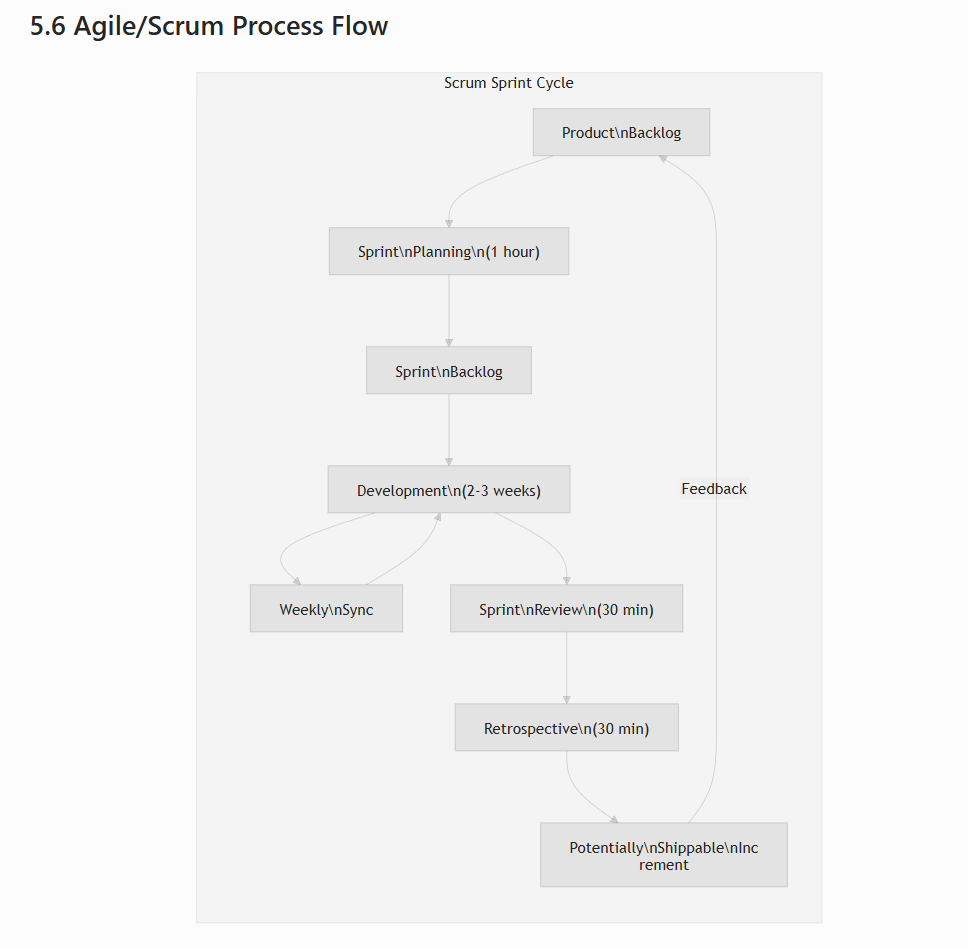
\includegraphics[width=0.9\textwidth,keepaspectratio]{Agile Process Diagram.png}
\caption{Agile/Scrum process diagram showing sprint cycles, backlog refinement, and iterative delivery within the 8-week development window.}
\label{fig:agile-process}
\end{figure}

Key parameters of our Agile implementation:
\begin{itemize}[noitemsep]
\item \textbf{Sprint Duration:} 2--3 weeks per sprint (3 sprints total)
\item \textbf{Team Size:} 2 developers (thesis project)
\item \textbf{Weekly Sync:} Progress review, blocker identification, and planning (replaces daily standup for a 2-person team)
\item \textbf{Sprint Planning:} 1 hour at sprint start
\item \textbf{Sprint Review and Retrospective:} 30 minutes each at sprint end
\end{itemize}

\vspace{8pt}
\begin{tcolorbox}[
    colback=PrimaryBlue!5,
    colframe=PrimaryBlue,
    coltitle=white,
    fonttitle=\bfseries\small,
    title={\centering AGILE DEVELOPMENT LIFECYCLE --- 2-Month Window},
    boxrule=0.8pt,
    arc=4pt,
]
\begin{center}
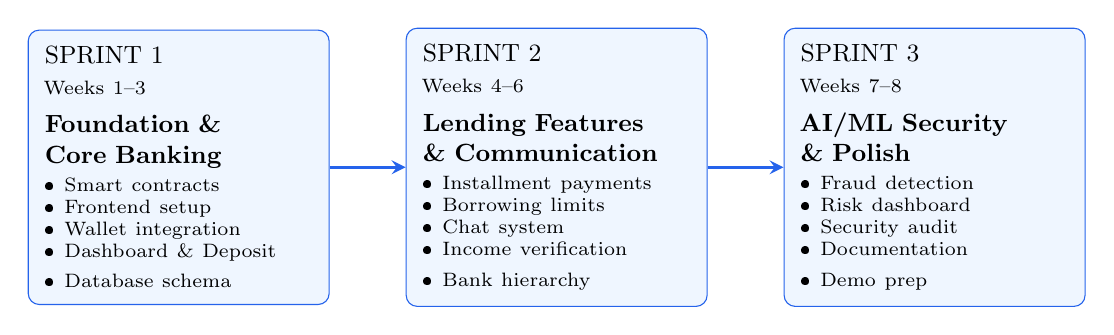
\begin{tikzpicture}[
    sprint/.style={
        draw=AccentBlue,
        fill=LightBlue,
        rounded corners=4pt,
        minimum width=3.6cm,
        minimum height=3.2cm,
        text width=3.4cm,
        align=left,
        font=\small,
        inner sep=6pt,
    },
    sprintlabel/.style={
        font=\bfseries\small,
        text=PrimaryBlue,
    },
    arrowstyle/.style={
        ->,
        >=stealth,
        line width=1.2pt,
        color=AccentBlue,
    }
]
\node[sprint] (s1) at (0,0) {
    {\sprintlabel SPRINT 1}\\
    {\scriptsize Weeks 1--3}\\[3pt]
    \textbf{Foundation \&}\\
    \textbf{Core Banking}\\[2pt]
    {\scriptsize
    \textbullet\ Smart contracts\\
    \textbullet\ Frontend setup\\
    \textbullet\ Wallet integration\\
    \textbullet\ Dashboard \& Deposit\\
    \textbullet\ Database schema}
};

\node[sprint] (s2) at (4.8,0) {
    {\sprintlabel SPRINT 2}\\
    {\scriptsize Weeks 4--6}\\[3pt]
    \textbf{Lending Features}\\
    \textbf{\& Communication}\\[2pt]
    {\scriptsize
    \textbullet\ Installment payments\\
    \textbullet\ Borrowing limits\\
    \textbullet\ Chat system\\
    \textbullet\ Income verification\\
    \textbullet\ Bank hierarchy}
};

\node[sprint] (s3) at (9.6,0) {
    {\sprintlabel SPRINT 3}\\
    {\scriptsize Weeks 7--8}\\[3pt]
    \textbf{AI/ML Security}\\
    \textbf{\& Polish}\\[2pt]
    {\scriptsize
    \textbullet\ Fraud detection\\
    \textbullet\ Risk dashboard\\
    \textbullet\ Security audit\\
    \textbullet\ Documentation\\
    \textbullet\ Demo prep}
};

\draw[arrowstyle] (s1.east) -- (s2.west);
\draw[arrowstyle] (s2.east) -- (s3.west);
\end{tikzpicture}
\end{center}
\end{tcolorbox}
\vspace{8pt}

\begin{figure}[H]
\centering
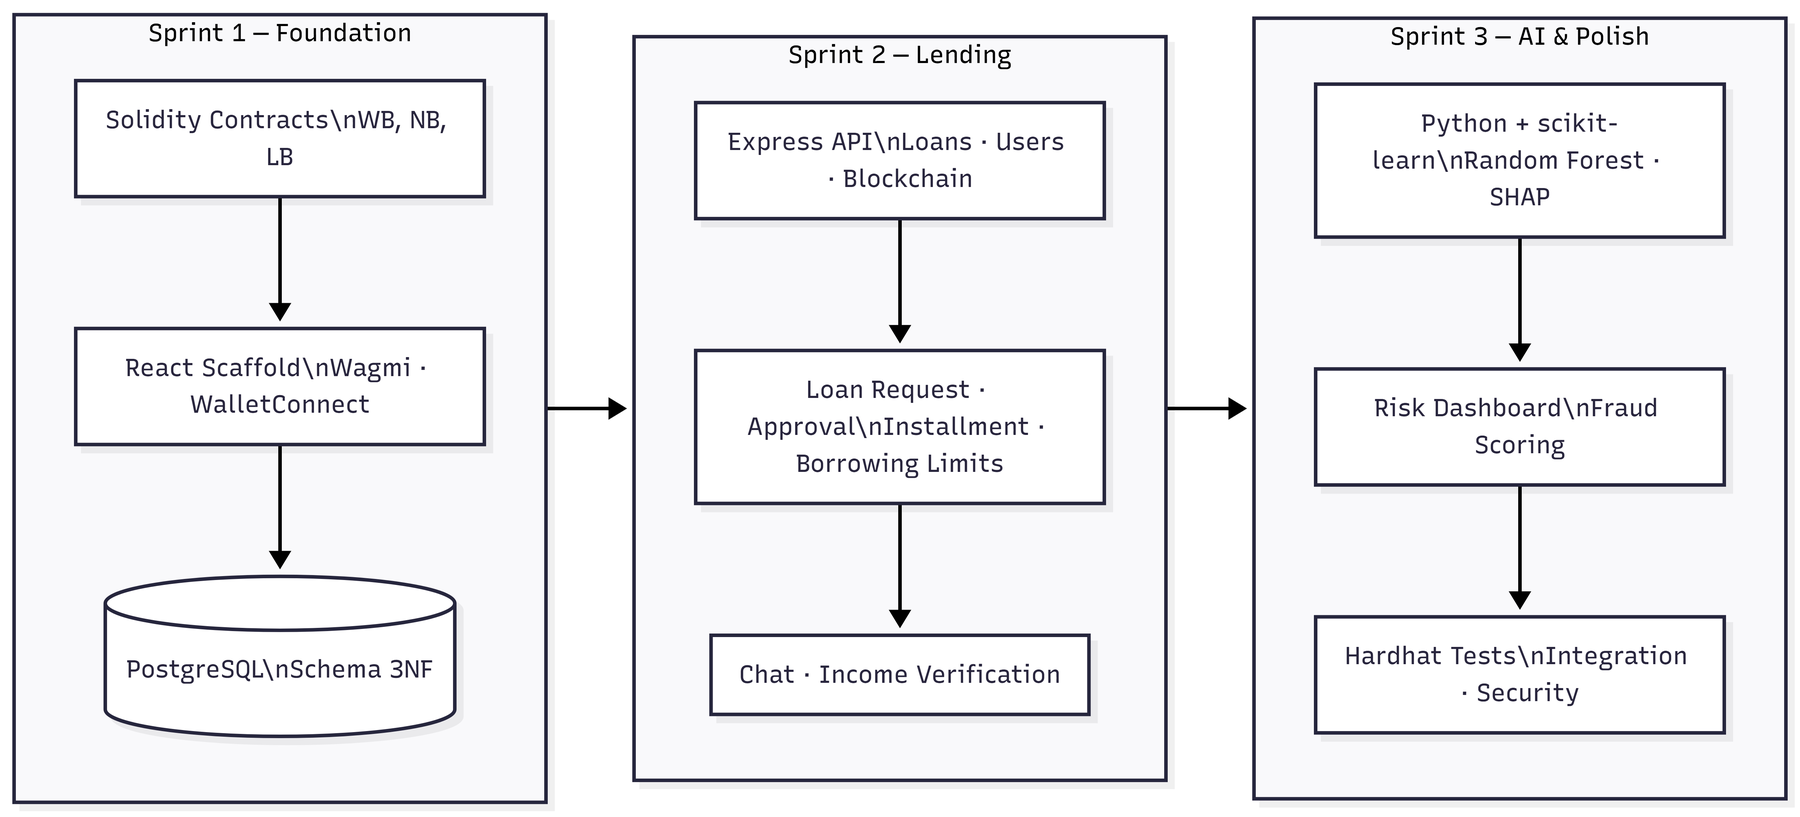
\includegraphics[height=7.5cm,keepaspectratio]{Methodology.png}
\caption{Technical development methodology: blockchain (Solidity), frontend (React, Wagmi, WalletConnect), backend (Express API, PostgreSQL), and AI/ML (Python, scikit-learn, Random Forest, SHAP) components across the three sprints.}
\label{fig:methodology-technical}
\end{figure}


\section{Sprint Plan and Deliverables}

\subsection{Sprint 1: Foundation and Core Banking (Weeks 1--3)}

\textbf{Sprint Goal:} Establish core blockchain infrastructure and hierarchical banking structure.

\begin{moderntable}
\caption{Sprint 1 backlog: Smart contract development (21 pts).}
\begin{tabular}{@{} >{\raggedright}p{1.3cm} >{\raggedright}p{8.5cm} >{\centering\arraybackslash}p{1cm} @{}}
\toprule
\tableheadfont ID & \tableheadfont User Story & \tableheadfont Pts \\
\midrule
\rowcolor{RowShade}
US-1.1 & World Bank contract --- reserve management, national bank registration & 5 \\
US-1.2 & National Bank contract --- borrow from WB, lend to Local Banks & 5 \\
\rowcolor{RowShade}
US-1.3 & Local Bank contract --- borrow from NB, lend to users & 5 \\
US-1.4 & Role-based access control --- WB/NB/LB Admin, Bank User, Borrower & 3 \\
\rowcolor{RowShade}
US-1.5 & Gas cost management --- initiator pays; Polygon low-fee (\$0.001--0.01/tx) & 3 \\
\bottomrule
\end{tabular}
\end{moderntable}

\begin{moderntable}
\caption{Sprint 1 backlog: Frontend foundation (13 pts) and database schema (8 pts).}
\begin{tabular}{@{} >{\raggedright}p{1.3cm} >{\raggedright}p{8.5cm} >{\centering\arraybackslash}p{1cm} @{}}
\toprule
\tableheadfont ID & \tableheadfont User Story & \tableheadfont Pts \\
\midrule
\rowcolor{RowShade}
US-1.6 & Wallet connection --- MetaMask, WalletConnect, Sepolia/Mumbai & 3 \\
US-1.7 & Dashboard UI --- Material Design 3, responsive, blockchain-themed & 5 \\
\rowcolor{RowShade}
US-1.8 & Navigation and layout --- AppBar, role-based menu & 3 \\
US-1.9 & Blockchain visual elements --- tx hash display, security badges & 2 \\
\rowcolor{RowShade}
US-1.10 & Database design --- 15 tables, 3NF & 5 \\
US-1.11 & Migration scripts and seed data & 3 \\
\bottomrule
\end{tabular}
\end{moderntable}

\textbf{Sprint 1 Total:} 42 story points. Deliverables: smart contracts deployed on testnet, basic frontend with wallet connection, database schema implemented, role-based access control, dashboard UI.


\subsection{Sprint 2: Lending Features and Communication (Weeks 4--6)}

\textbf{Sprint Goal:} Implement complete lending workflow and communication features.

\begin{moderntable}
\caption{Sprint 2 backlog: Lending and communication features (50 pts).}
\begin{tabular}{@{} >{\raggedright}p{1.3cm} >{\raggedright}p{8.5cm} >{\centering\arraybackslash}p{1cm} @{}}
\toprule
\tableheadfont ID & \tableheadfont User Story & \tableheadfont Pts \\
\midrule
\rowcolor{RowShade}
US-2.1 & Loan request submission with blockchain transaction & 5 \\
US-2.2 & Loan approval and rejection workflow with bank approver & 5 \\
\rowcolor{RowShade}
US-2.3 & Installment payment system with automated schedule generation & 8 \\
US-2.4 & Borrowing limit engine (6-month and 1-year rolling windows) & 5 \\
\rowcolor{RowShade}
US-2.5 & Borrower--bank real-time chat system & 5 \\
US-2.6 & Income verification document upload and review & 5 \\
\rowcolor{RowShade}
US-2.7 & Hierarchical bank registration (National $\to$ Local) & 5 \\
US-2.8 & Bank user management and approver designation & 3 \\
\rowcolor{RowShade}
US-2.9 & Loan history and transaction tracking pages & 5 \\
US-2.10 & QR code generation for wallet addresses & 2 \\
\rowcolor{RowShade}
US-2.11 & Responsive UI polish and error handling & 2 \\
\bottomrule
\end{tabular}
\end{moderntable}


\subsection{Sprint 3: AI/ML Security and Finalization (Weeks 7--8)}

\textbf{Sprint Goal:} Integrate AI/ML analytics, complete testing, and prepare documentation.

\begin{moderntable}
\caption{Sprint 3 backlog: AI/ML security and finalization (38 pts).}
\begin{tabular}{@{} >{\raggedright}p{1.3cm} >{\raggedright}p{8.5cm} >{\centering\arraybackslash}p{1cm} @{}}
\toprule
\tableheadfont ID & \tableheadfont User Story & \tableheadfont Pts \\
\midrule
\rowcolor{RowShade}
US-3.1 & Random Forest fraud detection model training and deployment & 8 \\
US-3.2 & SHAP-based explainability for risk assessments & 5 \\
\rowcolor{RowShade}
US-3.3 & Isolation Forest anomaly detection for wallet behavior & 5 \\
US-3.4 & Risk dashboard with real-time AI/ML scores & 5 \\
\rowcolor{RowShade}
US-3.5 & AI chatbot for borrower assistance & 3 \\
US-3.6 & Market data visualization page & 3 \\
\rowcolor{RowShade}
US-3.7 & Profile and settings management & 2 \\
US-3.8 & Security audit and vulnerability assessment & 3 \\
\rowcolor{RowShade}
US-3.9 & Documentation and report finalization & 2 \\
US-3.10 & Demo preparation and presentation & 2 \\
\bottomrule
\end{tabular}
\end{moderntable}

Figure~\ref{fig:sprint-submission} shows the sprint submission workflow.

\begin{figure}[H]
\centering
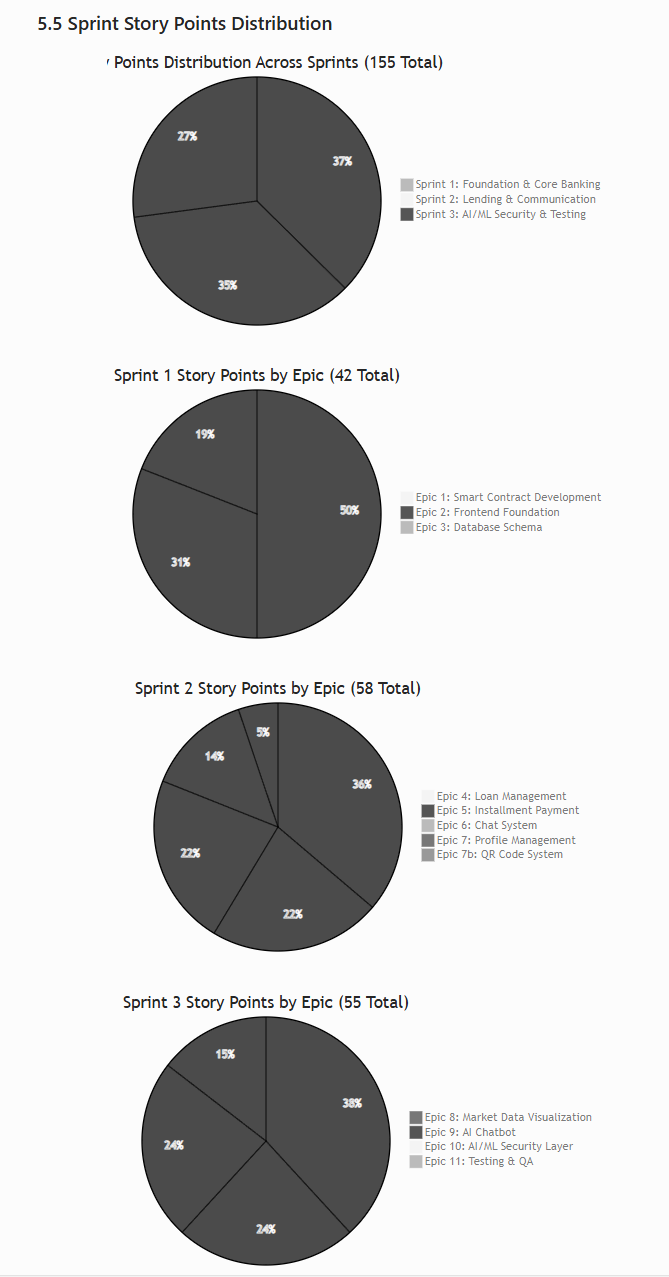
\includegraphics[width=0.85\textwidth,keepaspectratio]{Sprint submission Diagram.png}
\caption{Sprint submission diagram showing the workflow from backlog refinement through development, testing, review, and delivery for each sprint cycle.}
\label{fig:sprint-submission}
\end{figure}


\section{SDLC Stage Mapping}

We map our Agile sprints to the seven stages of the Software Development Life Cycle (SDLC). Figure~\ref{fig:sdlc-mapping} illustrates this mapping.

\begin{moderntable}
\caption{SDLC stage mapping.}
\begin{tabular}{@{} >{\raggedright}p{2.8cm} >{\raggedright}p{4.5cm} >{\raggedright\arraybackslash}p{4.5cm} @{}}
\toprule
\tableheadfont SDLC Stage & \tableheadfont Project Activity & \tableheadfont Deliverable \\
\midrule
\rowcolor{RowShade}
1. Planning & Feasibility studies; professor consultations; guideline review & Feasibility Report; Project Plan \\
2. Requirements & System analysis; use case definitions; constraints identification & Use case diagrams; UC-1 through UC-5 \\
\rowcolor{RowShade}
3. Design & Three-layer architecture; DB schema (3NF); smart contract interfaces & Architecture diagrams; ERD; DFD \\
4. Development & Sprint 1--3: smart contracts, frontend, backend, AI/ML & Source code; DApp prototype \\
\rowcolor{RowShade}
5. Testing & Hardhat unit tests (12+); integration testing; AI/ML evaluation & Test reports; model metrics \\
6. Deployment & Testnet deployment; frontend (Vercel); backend (Render) & Live prototype on testnet \\
\rowcolor{RowShade}
7. Maintenance & Monitoring; model retraining; bug fixes; iteration & Updated docs; retrained models \\
\bottomrule
\end{tabular}
\end{moderntable}

\begin{figure}[H]
\centering
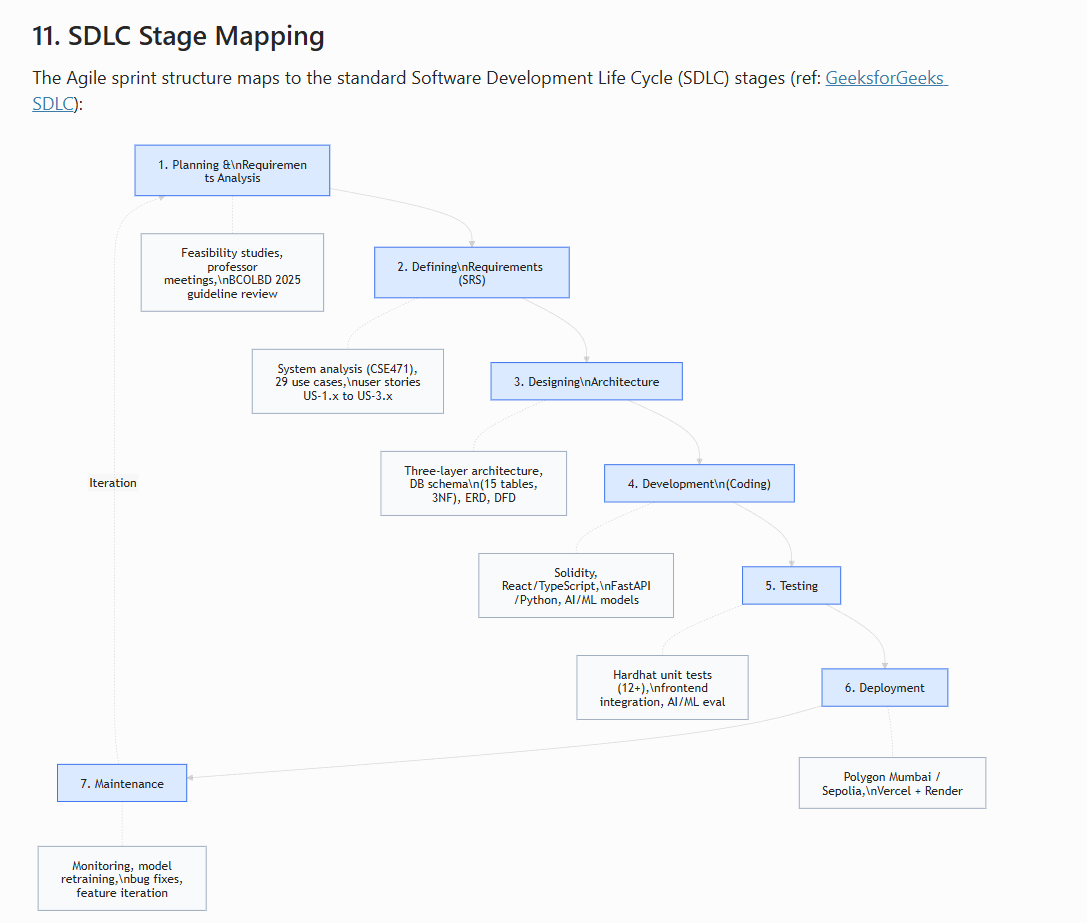
\includegraphics[width=0.9\textwidth,keepaspectratio]{SDLC stage mapping.png}
\caption{SDLC stage mapping diagram showing alignment between the seven SDLC stages and our three-sprint Agile methodology.}
\label{fig:sdlc-mapping}
\end{figure}


\section{Design Decisions and Alternatives}

For each major design decision, we evaluated alternatives and justified selections based on technical criteria, ecosystem maturity, and project constraints. Figure~\ref{fig:design-decisions} visualizes these comparisons.

\begin{moderntable}
\caption{Design decisions and alternatives considered.}
\begin{tabular}{@{} >{\raggedright}p{2.5cm} >{\raggedright}p{2.8cm} >{\raggedright}p{2.8cm} >{\raggedright\arraybackslash}p{3.5cm} @{}}
\toprule
\tableheadfont Decision Area & \tableheadfont 1st Choice & \tableheadfont 2nd Choice & \tableheadfont Key Criterion \\
\midrule
\rowcolor{RowShade}
Methodology & Agile / Scrum & Incremental & Evolving scope, milestones \\
Architecture & DApp + Off-chain AI & Hybrid w/ Oracle & Gas cost, ML flexibility \\
\rowcolor{RowShade}
Frontend & React + TypeScript & Vue + TypeScript & Web3 ecosystem maturity \\
Smart Contract & EVM (Solidity) & Solana (Rust) & Ecosystem size, free testnets \\
\rowcolor{RowShade}
UI Design & MUI (Material 3) & Tailwind CSS & Banking UI conventions \\
Fraud Detection & Random Forest & XGBoost & SHAP compatibility, 94\%+ precision \\
\rowcolor{RowShade}
Anomaly Detection & Isolation Forest & Autoencoder & Unsupervised, no labeled data needed \\
XAI Method & SHAP & LIME & Theoretical guarantees, regulatory fit \\
\rowcolor{RowShade}
Database & PostgreSQL & SQLite & 3NF support, async queries \\
Hosting & Vercel + Render & Localhost only & \$0 cost, publicly accessible URL \\
\bottomrule
\end{tabular}
\end{moderntable}

\begin{figure}[H]
\centering
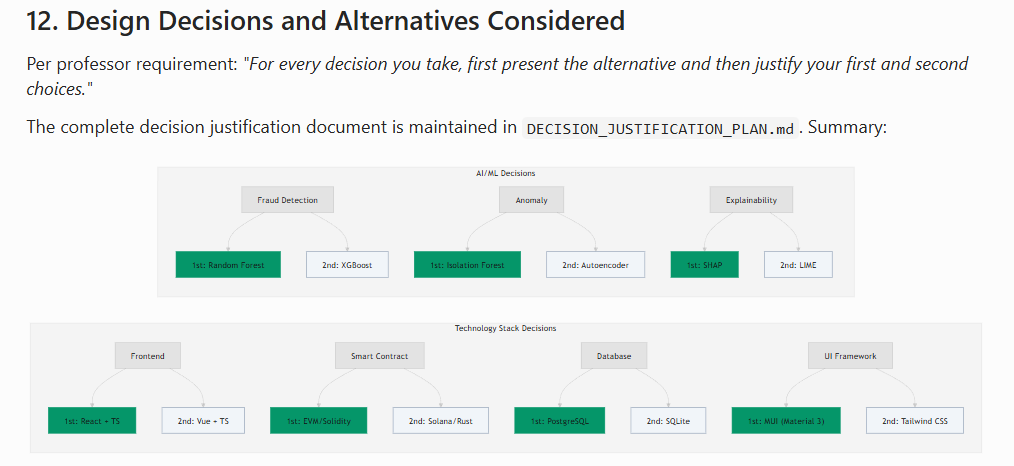
\includegraphics[width=0.9\textwidth,keepaspectratio]{Design Decisions and Alternatives Considered.png}
\caption{Design decisions and alternatives visualization across all major technology choices.}
\label{fig:design-decisions}
\end{figure}


\section{Design Patterns}

We applied three software design patterns in our architecture:

\begin{itemize}[noitemsep]
\item \textbf{Singleton:} Smart contract deployment follows the Singleton pattern---each contract (WorldBankReserve, NationalBank, LocalBank) is deployed once, and all participants interact with the same contract instance. This ensures a single source of truth for each tier's state.

\item \textbf{Observer:} The event-driven architecture uses the Observer pattern. Smart contracts emit events (e.g., \texttt{LoanRequested}, \texttt{LoanApproved}, \texttt{DepositMade}) that are consumed by the off-chain event listener service, which updates the PostgreSQL database and triggers UI notifications.

\item \textbf{Adapter:} The Web3 wallet integration layer implements the Adapter pattern via Wagmi and Viem, providing a unified interface across different wallet providers (MetaMask browser extension, WalletConnect mobile protocol) while adhering to the EIP-1193 standard.
\end{itemize}


\section{Software Testing Strategy}

Our testing strategy covers unit, integration, and model evaluation layers:

\begin{itemize}[noitemsep]
\item \textbf{Smart contract unit tests:} 12+ test cases written in Hardhat covering reserve management, hierarchical registration, loan lifecycle, access control violations, and edge cases (zero-amount deposits, unauthorized operations).
\item \textbf{Integration testing:} End-to-end workflow validation from wallet connection through loan request, approval, and installment repayment on testnet.
\item \textbf{AI/ML model evaluation:} Precision, recall, F1-score, and AUC-ROC metrics for the Random Forest fraud classifier; contamination threshold tuning for Isolation Forest; SHAP value consistency checks.
\item \textbf{Frontend testing:} Manual UI testing across Chrome, Firefox, and mobile viewports for responsive layout verification.
\end{itemize}


%% %%%%%%%%%%%%%%%%%%%%%%%%%%%%%%%%%%%%%%%%%%%%%%%%%%%%%%%%%%%%
%% CHAPTER 5: MARKET ANALYSIS AND FEASIBILITY
%% %%%%%%%%%%%%%%%%%%%%%%%%%%%%%%%%%%%%%%%%%%%%%%%%%%%%%%%%%%%%
\chapter{Market Analysis and Feasibility}

\section{Market Sizing}

\begin{moderntable}
\caption{Market segments.}
\begin{tabular}{@{} >{\raggedright}p{4cm} >{\raggedright}p{5cm} >{\raggedright\arraybackslash}p{3cm} @{}}
\toprule
\tableheadfont Segment & \tableheadfont Description & \tableheadfont Estimated Scale \\
\midrule
\rowcolor{RowShade}
Total Addressable Market (TAM) & Global decentralized lending market; DeFi lending TVL has historically exceeded \$50B & \$50B+ \\
Serviceable Addressable Market (SAM) & Institutional and semi-institutional lending requiring hierarchical structures & \$5--10B \\
\rowcolor{RowShade}
Serviceable Obtainable Market (SOM) & Pilot deployments in regulatory sandboxes, academic prototypes, NGO-backed microfinance & \$50--200M \\
\bottomrule
\end{tabular}
\end{moderntable}

\vspace{4pt}
\noindent\textit{\small\textbf{Sources:} (a)~TAM: DefiLlama~[13] tracks DeFi TVL; lending protocols have historically exceeded \$50B in total value locked; (b)~SAM and SOM: Project-derived estimates based on industry segmentation~[18].}

The market for \textbf{transparent, hierarchy-preserving decentralized lending} is presently unaddressed by existing DeFi protocols, which universally adopt flat, pool-based architectures. This represents a significant whitespace opportunity.

\section{Target Customer Segment}

The Crypto World Bank targets the \textbf{retail customer segment}---individual borrowers and small businesses seeking transparent, accessible crypto-based lending services.

\begin{moderntable}
\caption{Target customer segment profile.}
\begin{tabular}{@{} >{\raggedright}p{3.8cm} >{\raggedright\arraybackslash}p{8.2cm} @{}}
\toprule
\tableheadfont Characteristic & \tableheadfont Description \\
\midrule
\rowcolor{RowShade}
Primary Users & Individual retail borrowers seeking personal or small business loans \\
Geographic Focus & Developing economies with limited traditional banking access (e.g., Bangladesh, Southeast Asia, Sub-Saharan Africa) \\
\rowcolor{RowShade}
Loan Size Range & Micro to mid-range: 0.1 ETH -- 500 ETH equivalent (\textasciitilde\$200 -- \$1,000,000 at current rates) \\
User Profile & Digitally literate individuals with cryptocurrency wallet access; small business owners; gig-economy freelancers \\
\rowcolor{RowShade}
Key Pain Points & High interest rates from informal lenders; lack of credit history; exclusion from banking due to documentation barriers \\
\bottomrule
\end{tabular}
\end{moderntable}

\section{Partner Ecosystem}

\begin{moderntable}
\caption{Partner categories and roles.}
\begin{tabular}{@{} >{\raggedright}p{3.2cm} >{\raggedright}p{4.2cm} >{\raggedright\arraybackslash}p{4.6cm} @{}}
\toprule
\tableheadfont Partner Category & \tableheadfont Functional Role & \tableheadfont Blockchain-Mediated Incentive \\
\midrule
\rowcolor{RowShade}
Financial Regulators & Regulatory sandbox approval; compliance oversight & Reduced enforcement cost through on-chain transparency \\
Banking Institutions & Network membership as National/Local Banks & Access to diversified global reserve; reduced settlement friction \\
\rowcolor{RowShade}
Payment Gateways & Fiat-to-crypto on-ramp and off-ramp services & Volume-based transaction fees; expanded market reach \\
Academic Institutions & Validation of AI/ML models; research publication & Access to anonymized datasets; collaborative opportunities \\
\rowcolor{RowShade}
NGOs & Pilot deployment with underserved populations & Transparent, low-friction credit access for beneficiaries \\
\bottomrule
\end{tabular}
\end{moderntable}


\section{Competitive Landscape}

\begin{moderntable}
\caption{Direct competition and differentiation.}
\begin{tabular}{@{} >{\raggedright}p{2.8cm} >{\raggedright}p{3.4cm} >{\raggedright\arraybackslash}p{5.5cm} @{}}
\toprule
\tableheadfont Competitor Category & \tableheadfont Examples & \tableheadfont Our Differentiation \\
\midrule
\rowcolor{RowShade}
DeFi lending protocols & Aave, Compound, MakerDAO & Four-tier institutional model; integrated AI/ML risk layer; role-based governance \\
Traditional development finance & World Bank, IFC, ADB & On-chain transparency; programmable enforcement; near-instant settlement \\
\rowcolor{RowShade}
Blockchain credit platforms & Centrifuge, Maple, Goldfinch & Combined hierarchy and AI security; designed for institutional adoption \\
\bottomrule
\end{tabular}
\end{moderntable}

\begin{itemize}[noitemsep]
\item \textbf{Central Bank Digital Currencies (CBDCs):} Emerging CBDC frameworks may address settlement efficiency but do not provide decentralized lending capabilities. Our platform positions as a complementary \textbf{lending layer} operating on top of digital asset infrastructure.
\item \textbf{Peer-to-peer lending platforms:} Predominantly fiat-denominated and centralized; the Crypto World Bank targets crypto-native and hybrid institutional use cases.
\end{itemize}

\section{Risk Taxonomy}

\begin{moderntable}
\caption{Risk taxonomy and mitigation strategy.}
\begin{tabular}{@{} >{\raggedright}p{2.4cm} >{\raggedright}p{3.2cm} >{\centering\arraybackslash}p{1.8cm} >{\raggedright\arraybackslash}p{4.2cm} @{}}
\toprule
\tableheadfont Risk Category & \tableheadfont Description & \tableheadfont Severity & \tableheadfont Mitigation \\
\midrule
\rowcolor{RowShade}
Partner non-cooperation & Key partners decline to participate & {\color{AmberAccent}\textbf{Medium}} & Initiate with low-barrier academic and NGO pilots \\
Smart contract vulnerability & Exploit in contract logic & {\color{RedAccent}\textbf{High}} & OpenZeppelin primitives; formal audit (planned); pause mechanism \\
\rowcolor{RowShade}
Regulatory adversity & Jurisdictional restrictions & {\color{AmberAccent}\textbf{Medium}} & Testnet-only prototype; regulatory sandbox engagement \\
AI/ML model degradation & Fraud detection accuracy decay & {\color{GreenAccent}\textbf{Low}} & Continuous retraining; human-in-the-loop; SHAP explainability \\
\bottomrule
\end{tabular}
\end{moderntable}


\section{Technical Feasibility}

\begin{moderntable}
\caption{Technical feasibility assessment.}
\begin{tabular}{@{} >{\raggedright}p{2.5cm} >{\raggedright}p{2.2cm} >{\raggedright\arraybackslash}p{7cm} @{}}
\toprule
\tableheadfont Component & \tableheadfont Assessment & \tableheadfont Evidence \\
\midrule
\rowcolor{RowShade}
Smart contracts & {\color{GreenAccent}\textbf{Fully feasible}} & Three contracts implemented, compiled, and tested with Hardhat (12+ passing unit tests); Solidity 0.8.20 with OpenZeppelin \\
Frontend DApp & {\color{GreenAccent}\textbf{Fully feasible}} & React 18 + TypeScript with all pages implemented; Wagmi and RainbowKit provide mature wallet integration \\
\rowcolor{RowShade}
Blockchain deployment & {\color{GreenAccent}\textbf{Fully feasible}} & Polygon Mumbai and Ethereum Sepolia provide zero-cost, production-equivalent environments \\
AI/ML integration & {\color{AmberAccent}\textbf{Feasible w/ constraints}} & Random Forest inference achieves sub-50ms latency; SHAP explanations computable in real-time \\
\rowcolor{RowShade}
Database backend & {\color{GreenAccent}\textbf{Feasible}} & PostgreSQL schema designed (15 tables, 3NF); FastAPI provides async REST framework \\
\bottomrule
\end{tabular}
\end{moderntable}


\section{Economic Feasibility}

\begin{moderntable}
\caption{Economic feasibility --- zero-cost prototype.}
\begin{tabular}{@{} >{\raggedright}p{3.5cm} >{\raggedright}p{3cm} >{\raggedright\arraybackslash}p{5.5cm} @{}}
\toprule
\tableheadfont Cost Category & \tableheadfont Estimate & \tableheadfont Notes \\
\midrule
\rowcolor{RowShade}
Blockchain deployment & \$0 & Public testnets --- no real cryptocurrency required \\
Frontend hosting & \$0 & Vercel free tier or localhost for demo \\
\rowcolor{RowShade}
Backend hosting & \$0 & Render free tier or localhost \\
AI/ML training & \$0 & Local machine (16\,GB RAM, 16\,GB VRAM) or Google Colab free tier \\
\rowcolor{RowShade}
Development tools & \$0 & Hardhat, VS Code, Git --- all open-source \\
\textbf{Total prototype cost} & \textbf{\$0} & Entire prototype operates at zero financial cost \\
\bottomrule
\end{tabular}
\end{moderntable}


\section{Revenue Projection}

The following projection models annual revenue potential at full deployment scale. Calculations use a reference ETH price of \textbf{\$2,000} (February 2026 market rate) and interest rate parameters defined in Section~\ref{sec:interest-rates}.

\begin{moderntable}
\caption{Revenue projection assumptions.}
\begin{tabular}{@{} >{\raggedright}p{5.5cm} >{\raggedright\arraybackslash}p{6.5cm} @{}}
\toprule
\tableheadfont Parameter & \tableheadfont Value \\
\midrule
\rowcolor{RowShade}
Reference ETH price & \$2,000 (Feb 2026) \\
World Bank $\to$ National Bank rate & 3\% APR (wholesale inter-bank) \\
\rowcolor{RowShade}
National Bank $\to$ Local Bank rate & 5\% APR (inter-bank) \\
Local Bank $\to$ Borrower rate & 8\% APR (retail lending) \\
\rowcolor{RowShade}
Average loan term & 12 months \\
Default rate provision & 3\% (conservative estimate) \\
\rowcolor{RowShade}
Origination fee & 0.25\% per disbursement \\
\bottomrule
\end{tabular}
\end{moderntable}

\begin{moderntable}
\caption{System-wide annual revenue summary.}
\begin{tabular}{@{} >{\raggedright}p{5.5cm} r r @{}}
\toprule
\tableheadfont Tier & \tableheadfont Annual Revenue (ETH) & \tableheadfont USD Equivalent \\
\midrule
\rowcolor{RowShade}
Tier 1: World Bank (1 entity) & 31,525 & \$63,050,000 \\
Tier 2: National Banks (5 entities) & 25,775 & \$51,550,000 \\
\rowcolor{RowShade}
Tier 3: Local Banks (50 entities) & 55,025 & \$110,050,000 \\
\midrule
\rowcolor{MidBlue}
\textbf{Total platform revenue} & \textbf{112,325} & \textbf{\$224,650,000} \\
Borrower surplus generated & 70,000--120,000 & \$140M--240M \\
\bottomrule
\end{tabular}
\end{moderntable}

\vspace{4pt}
\noindent\textit{\small\textbf{Sources:} ETH price from spot market data (CoinGecko); interest rate tiers aligned with Aave~[15] and Compound~[16] DeFi benchmarks; default rate and origination fee from conservative industry estimates.}

\begin{figure}[H]
\centering
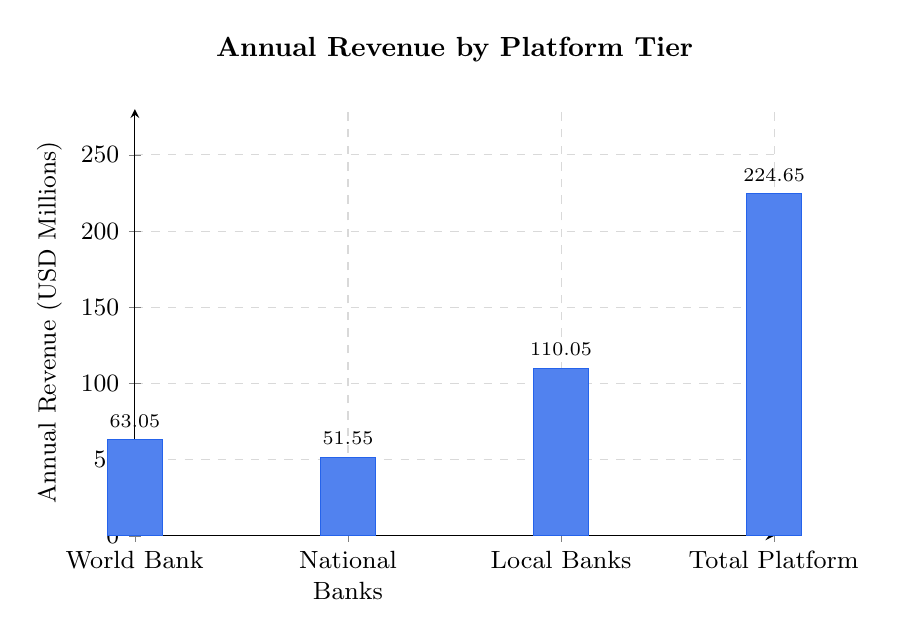
\begin{tikzpicture}
\begin{axis}[
    ybar,
    bar width=20pt,
    width=0.80\textwidth,
    height=7cm,
    clip=false,
    ylabel={Annual Revenue (USD Millions)},
    ylabel style={font=\small},
    symbolic x coords={World Bank,National Banks,Local Banks,Total Platform},
    xtick=data,
    xticklabel style={font=\small,text width=2.2cm,align=center},
    yticklabel style={font=\small},
    ymin=0,
    ymax=280,
    ytick={0,50,100,150,200,250},
    nodes near coords,
    nodes near coords style={font=\scriptsize\bfseries},
    every node near coord/.append style={anchor=south,yshift=1pt},
    enlarge x limits=0.22,
    grid=major,
    grid style={dashed,gray!30},
    axis lines=left,
    title={\textbf{Annual Revenue by Platform Tier}},
    title style={font=\normalsize,at={(0.5,1.05)}},
]
\addplot[fill=AccentBlue!80,draw=AccentBlue] coordinates {
    (World Bank,63.05) (National Banks,51.55) (Local Banks,110.05) (Total Platform,224.65)
};
\end{axis}
\end{tikzpicture}
\caption{Annual revenue projection by tier (USD millions, at \$2{,}000/ETH).}
\end{figure}

\subsection{Transaction Economics: Interest Rates}
\label{sec:interest-rates}

\begin{moderntable}
\caption{Interest rate parameters.}
\begin{tabular}{@{} >{\raggedright}p{3.5cm} >{\raggedright}p{3.5cm} >{\raggedright\arraybackslash}p{5cm} @{}}
\toprule
\tableheadfont Parameter & \tableheadfont Value & \tableheadfont Benchmark \\
\midrule
\rowcolor{RowShade}
Base Annual Interest Rate & 5--12\% APR & Aligned with Aave/Compound variable rates \\
Rate Determination & Set by Local Bank approvers within World Bank-defined bounds & Configurable per-bank for local market conditions \\
\rowcolor{RowShade}
Late Payment Penalty & 2\% of installment + 0.5\%/week (capped at 10\%) & Industry-standard late fee structure \\
Interest Calculation & Simple interest on outstanding principal & Transparent, borrower-friendly \\
\rowcolor{RowShade}
Rate Transparency & All parameters stored on-chain & Publicly auditable; no hidden fees \\
\bottomrule
\end{tabular}
\end{moderntable}

\begin{figure}[H]
\centering
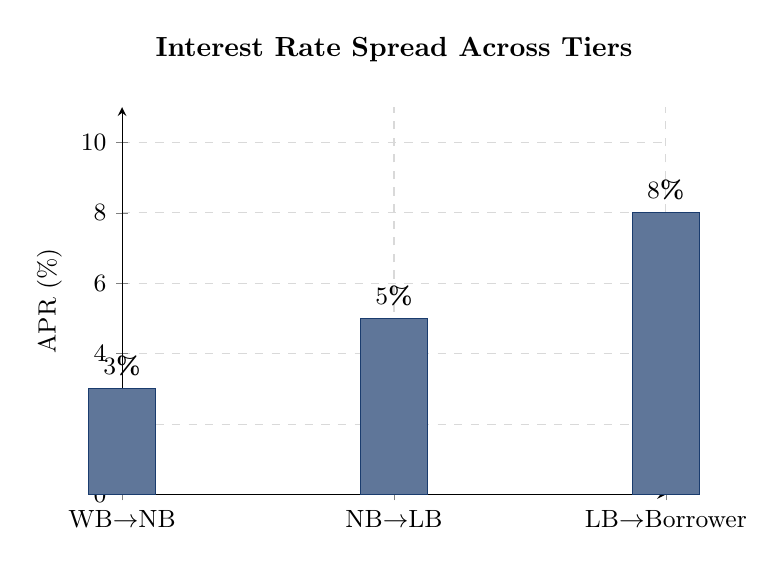
\begin{tikzpicture}
\begin{axis}[
    ybar,
    bar width=24pt,
    width=0.70\textwidth,
    height=6.5cm,
    clip=false,
    ylabel={APR (\%)},
    ylabel style={font=\small},
    symbolic x coords={WB$\to$NB,NB$\to$LB,LB$\to$Borrower},
    xtick=data,
    xticklabel style={font=\small},
    yticklabel style={font=\small},
    ymin=0,
    ymax=11,
    ytick={0,2,4,6,8,10},
    nodes near coords={\pgfmathprintnumber\pgfplotspointmeta\%},
    nodes near coords style={font=\small\bfseries},
    every node near coord/.append style={anchor=south,yshift=1pt},
    enlarge x limits=0.4,
    grid=major,
    grid style={dashed,gray!30},
    axis lines=left,
    title={\textbf{Interest Rate Spread Across Tiers}},
    title style={font=\normalsize,at={(0.5,1.05)}},
]
\addplot[fill=PrimaryBlue!70,draw=PrimaryBlue] coordinates {
    (WB$\to$NB,3) (NB$\to$LB,5) (LB$\to$Borrower,8)
};
\end{axis}
\end{tikzpicture}
\caption{Hierarchical interest rate spread (APR) across the four-tier lending structure.}
\end{figure}

\subsection{Global Economic Impact}

Beyond direct platform revenue, the Crypto World Bank creates broader economic value:

\begin{itemize}[noitemsep]
\item \textbf{Capital deployment:} \$2 billion in lending capital reaches 1,000 direct borrowers across developing economies. World Bank research~[19] indicates that each dollar of institutional lending generates approximately \$2.5--3.0 in downstream economic activity, implying a potential \textbf{\$5--6 billion annual economic stimulus}.
\item \textbf{Job creation:} SME lending research (IFC, 2019)~[20] estimates that every \$50,000 in small business credit creates or sustains one job, suggesting support for an estimated \textbf{40,000 direct jobs}.
\item \textbf{Financial inclusion:} The platform's retail-focused design provides transparent, accessible credit to underserved populations without requiring traditional banking relationships or credit histories.
\item \textbf{Transaction cost reduction:} On Polygon PoS, transaction fees remain below \$0.01, representing a \textbf{60--80\% cost reduction} compared to traditional correspondent banking~[21].
\end{itemize}

\subsection{Value Proposition and Go-to-Market}

\begin{moderntable}
\caption{Go-to-market phases.}
\begin{tabular}{@{} >{\raggedright}p{3cm} >{\raggedright}p{6.5cm} >{\raggedright\arraybackslash}p{2.5cm} @{}}
\toprule
\tableheadfont Phase & \tableheadfont Activities & \tableheadfont Timeline \\
\midrule
\rowcolor{RowShade}
Phase 1: Validation & Competition submission (BCOLBD 2025); thesis publication; open-source release & Current \\
Phase 2: Pilot & Regulatory sandbox application; institutional partnership; testnet-to-mainnet migration & 6--12 months \\
\rowcolor{RowShade}
Phase 3: Production & Multi-chain deployment; full AI/ML backend; governance token launch & 12--24 months \\
\bottomrule
\end{tabular}
\end{moderntable}


%% %%%%%%%%%%%%%%%%%%%%%%%%%%%%%%%%%%%%%%%%%%%%%%%%%%%%%%%%%%%%
%% CHAPTER 6: CONCLUSION
%% %%%%%%%%%%%%%%%%%%%%%%%%%%%%%%%%%%%%%%%%%%%%%%%%%%%%%%%%%%%%
\chapter{Conclusion}

The Crypto World Bank addresses a \textbf{complex, multi-party coordination and trust problem} in hierarchical development finance by leveraging the unique properties of blockchain technology: immutability, programmable enforcement, and cryptographic auditability. Our solution goes beyond existing DeFi lending protocols by introducing a four-tier institutional hierarchy, AI/ML-augmented risk assessment, and a governance framework that addresses network membership, business operations, and technology infrastructure.

The platform is positioned at the intersection of decentralized finance, institutional lending, and applied AI security---a combination that is presently unaddressed in both the academic literature and the commercial blockchain landscape. With a working prototype, a defined market and partnership strategy, transparent risk assessment, and a phased go-to-market plan, the Crypto World Bank represents a viable and scalable contribution to the emerging field of blockchain-based development finance.

Future work will focus on: (1)~mainnet deployment with real asset testing in regulatory sandbox environments; (2)~expanded AI/ML capabilities including reinforcement learning for dynamic interest rate optimization; (3)~cross-chain interoperability for multi-network lending; and (4)~formal security verification of all smart contract code using tools such as Slither and Mythril.


%% %%%%%%%%%%%%%%%%%%%%%%%%%%%%%%%%%%%%%%%%%%%%%%%%%%%%%%%%%%%%
%% APPENDICES
%% %%%%%%%%%%%%%%%%%%%%%%%%%%%%%%%%%%%%%%%%%%%%%%%%%%%%%%%%%%%%
\appendix

\chapter{Technology Stack}

\begin{moderntable}
\caption{Technology stack summary.}
\begin{tabular}{@{} >{\raggedright}p{3cm} >{\raggedright}p{4.5cm} >{\raggedright\arraybackslash}p{4.5cm} @{}}
\toprule
\tableheadfont Layer & \tableheadfont Technology & \tableheadfont Version / Notes \\
\midrule
\rowcolor{RowShade}
Smart Contract & Solidity, OpenZeppelin & 0.8.20; Ownable, ReentrancyGuard \\
Frontend & React, TypeScript, Vite, Material-UI & React 18; MUI v5; Material Design 3 \\
\rowcolor{RowShade}
Wallet Integration & Wagmi, RainbowKit, Viem & EIP-1193 compliant \\
Build and Test & Hardhat & Automated test suite; deployment scripts \\
\rowcolor{RowShade}
Target Networks & Polygon Mumbai, Ethereum Sepolia & Public testnets; zero-cost \\
AI/ML (planned) & Python, FastAPI, scikit-learn, SHAP & Random Forest, Isolation Forest, SHAP \\
\bottomrule
\end{tabular}
\end{moderntable}

\chapter{Smart Contract Capabilities}

The platform's three smart contracts collectively support the following operations:

\begin{itemize}[noitemsep]
\item \textbf{World Bank Reserve Contract:} Reserve management, deposit handling, national bank registration, fund distribution to national banks, system pause/unpause, emergency withdrawal, and global statistics.
\item \textbf{National Bank Contract:} Local bank registration, borrowing from the world bank reserve, fund distribution to local banks, and network status queries.
\item \textbf{Local Bank Contract:} Loan requests, loan approval and rejection, installment payments, bank user management, and approver designation.
\end{itemize}


%% %%%%%%%%%%%%%%%%%%%%%%%%%%%%%%%%%%%%%%%%%%%%%%%%%%%%%%%%%%%%
%% REFERENCES
%% %%%%%%%%%%%%%%%%%%%%%%%%%%%%%%%%%%%%%%%%%%%%%%%%%%%%%%%%%%%%
\chapter*{References}
\addcontentsline{toc}{chapter}{References}

{\small
\begin{enumerate}[label={[\arabic*]}]
\item S.~M. Werner, D.~Perez, L.~Gudgeon, A.~Klages-Mundt, D.~Harz, and W.~J. Knottenbelt, ``SoK: Decentralized Finance (DeFi),'' \textit{arXiv preprint arXiv:2101.08778}, 2022. [Online]. Available: \url{https://arxiv.org/abs/2101.08778}

\item S.~Bastankhah, M.~Hashemi, and W.~Shi, ``An Adaptive Data-Driven DeFi Borrow-Lending Protocol,'' \textit{Proc. IEEE Int. Conf. Blockchain}, 2023.

\item G.~Palaiokrassas, A.~Skoufis, and L.~Tassiulas, ``Leveraging Machine Learning for Multichain DeFi Fraud Detection,'' \textit{Proc. IEEE Int. Conf. Blockchain and Cryptocurrency (ICBC)}, 2023.

\item D.~Adom, E.~O. Acheampong, and M.~Boateng, ``LIME and SHAP: A Comparison of Model-Agnostic Approaches to Explainability in Loan Approval Systems,'' \textit{International Journal of Advanced Computer Science and Applications}, vol.~13, no.~11, 2022.

\item B.~W. Tan, ``Central Bank Digital Currency and Financial Inclusion,'' \textit{IMF Working Paper WP/23/69}, 2023. [Online]. Available: \url{https://www.imf.org/en/Publications/WP}

\item F.~T. Liu, K.~M. Ting, and Z.-H. Zhou, ``Isolation Forest,'' in \textit{Proc. IEEE Int. Conf. Data Mining (ICDM)}, pp.~413--422, 2008. DOI: \url{https://doi.org/10.1109/ICDM.2008.17}

\item N.~Atzei, M.~Bartoletti, and T.~Cimoli, ``A Survey of Attacks on Ethereum Smart Contracts (SoK),'' in \textit{Proc. Int. Conf. Principles of Security and Trust (POST)}, pp.~164--186, 2017. DOI: \url{https://doi.org/10.1007/978-3-662-54455-6_8}

\item S.~M. Lundberg and S.-I. Lee, ``A Unified Approach to Interpreting Model Predictions,'' in \textit{Advances in Neural Information Processing Systems (NeurIPS)}, pp.~4765--4774, 2017. [Online]. Available: \url{https://proceedings.neurips.cc/paper/2017/hash/8a20a8621978632d76c43dfd28b67767-Abstract.html}

\item P.~Bracke, A.~Datta, C.~Jung, and S.~Sen, ``Machine Learning Explainability in Finance: An Application to Default Risk Analysis,'' \textit{Bank of England Staff Working Paper No.~816}, 2019. [Online]. Available: \url{https://www.bankofengland.co.uk/working-paper/2019/machine-learning-explainability-in-finance}

\item R.~Beck, C.~M\"{u}ller-Bloch, and J.~L. King, ``Governance in the Blockchain Economy: A Framework and Research Agenda,'' \textit{Journal of the Association for Information Systems}, vol.~19, no.~10, pp.~1020--1034, 2018. DOI: \url{https://doi.org/10.17705/1jais.00518}

\item D.~Mhlanga, ``Blockchain Technology for Financial Inclusion and Sustainable Development,'' in \textit{Digital Financial Inclusion}, Springer, 2022.

\item OpenZeppelin, ``OpenZeppelin Contracts,'' 2024. [Online]. Available: \url{https://openzeppelin.com/contracts}

\item DefiLlama, ``Lending Protocols --- DeFi TVL and Protocol Rankings,'' 2024--2025. [Online]. Available: \url{https://defillama.com/protocols/lending}

\item World Bank, ``The Global Findex Database 2021: Financial Inclusion, Digital Payments, and Resilience,'' 2021. [Online]. Available: \url{https://www.worldbank.org/en/publication/globalfindex}

\item Aave, ``Aave Protocol Documentation,'' 2024. [Online]. Available: \url{https://docs.aave.com/}

\item Compound, ``Compound Protocol Documentation,'' 2024. [Online]. Available: \url{https://docs.compound.finance/}

\item BCOLBD 2025, ``Blockchain Olympiad Bangladesh: Guideline and Evaluation Scheme,'' 2025. [Online]. Available: \url{https://bcolbd.org/uploads/guideline/BLOCKCHAIN\%20OLYMPIAD\%20BANGLADESH\%20Blockchain\%20Guideline.pdf}

\item Galaxy Digital, ``The State of Crypto Lending and Borrowing,'' Galaxy Research, 2024. [Online]. Available: \url{https://www.galaxy.com/insights/research/the-state-of-crypto-lending}

\item World Bank, ``World Development Report 2022: Finance for an Equitable Recovery,'' 2022. [Online]. Available: \url{https://www.worldbank.org/en/publication/wdr2022}

\item International Finance Corporation (IFC), ``MSME Finance Gap 2019,'' 2019. [Online]. Available: \url{https://www.ifc.org/en/insights-reports/2019/msme-finance-gap}

\item Bank for International Settlements, ``DeFi Lending: Intermediation Without Information?,'' BIS Working Paper No.~1183, 2024. [Online]. Available: \url{https://www.bis.org/publ/work1183.pdf}

\item Deloitte, ``Global Banking Outlook 2024,'' 2024.

\item Michigan State University Libraries, ``Literature Table and Synthesis --- Nursing Literature Reviews,'' LibGuides, 2025. [Online]. Available: \url{https://libguides.lib.msu.edu/nursinglitreview/table}
\end{enumerate}
}

\end{document}
